\chapter{Searches for supersymmetry at $\sqrt{s}=13\TeV$}
\label{ch:analysis13TeV}

Searches for SUSY performed using $\Pp\Pp$ collision data collected in 2012 at $\sqrt{s}=8\TeV$ by ATLAS
~\cite{Aad:2013wta,Aad:2014lra,Aad:2014pda,Aad:2014bva,Aad:2014qaa,Atlas3rdGen,Atlas8tevSummary,Aad:2015mia}
and
CMS~\cite{1LepMVA,SUS12024,Chatrchyan:2014lfa,Chatrchyan:2013iqa,Chatrchyan:2013fea,Chatrchyan:2013lya,MT2at8TeV},
including the inclusive razor search described in
Ch.~\ref{ch:analysis8TeV}~\cite{razor8TeV}, have probed SUSY particle masses near the TeV
scale.

In early 2015, the LHC restarted $\Pp\Pp$ collisions at a collision
energy of 13 \TeV after two years of maintenance and upgrades.
The increase in center-of-mass energy from 8 to 13 \TeV provides an opportunity to
significantly extend the sensitivity of LHC searches to higher SUSY particle
masses~\cite{Khachatryan:2016kdk,
  Khachatryan:2016xvy, Khachatryan:2016uwr, Khachatryan:2016kod,
  Khachatryan:2016fll, Aad:2016jxj, Aad:2016tuk, Aaboud:2016tnv, Aaboud:2016zdn,
  Aad:2016qqk, Aad:2016eki, Aaboud:2016lwz, Aaboud:2016nwl,
  ATLASCollaboration:2016wlb}. In particular, the largest gain in
sensitivity is expected for gluinos, which would be produced almost
$50$ times more often at 13 \TeV than at 8 \TeV for a gluino
mass of $1.6\TeV$. Top squarks, on the other hand would only be
produced at a rate $10$ times larger for a top squark mass of $800
\GeV$. Fig.~\ref{fig:gluinostop13TeV8TeV} shows the pair production
cross sections for gluinos and top squarks at 8 and 13\TeV as
well as their ratio.

\begin{figure}[!htb] \centering
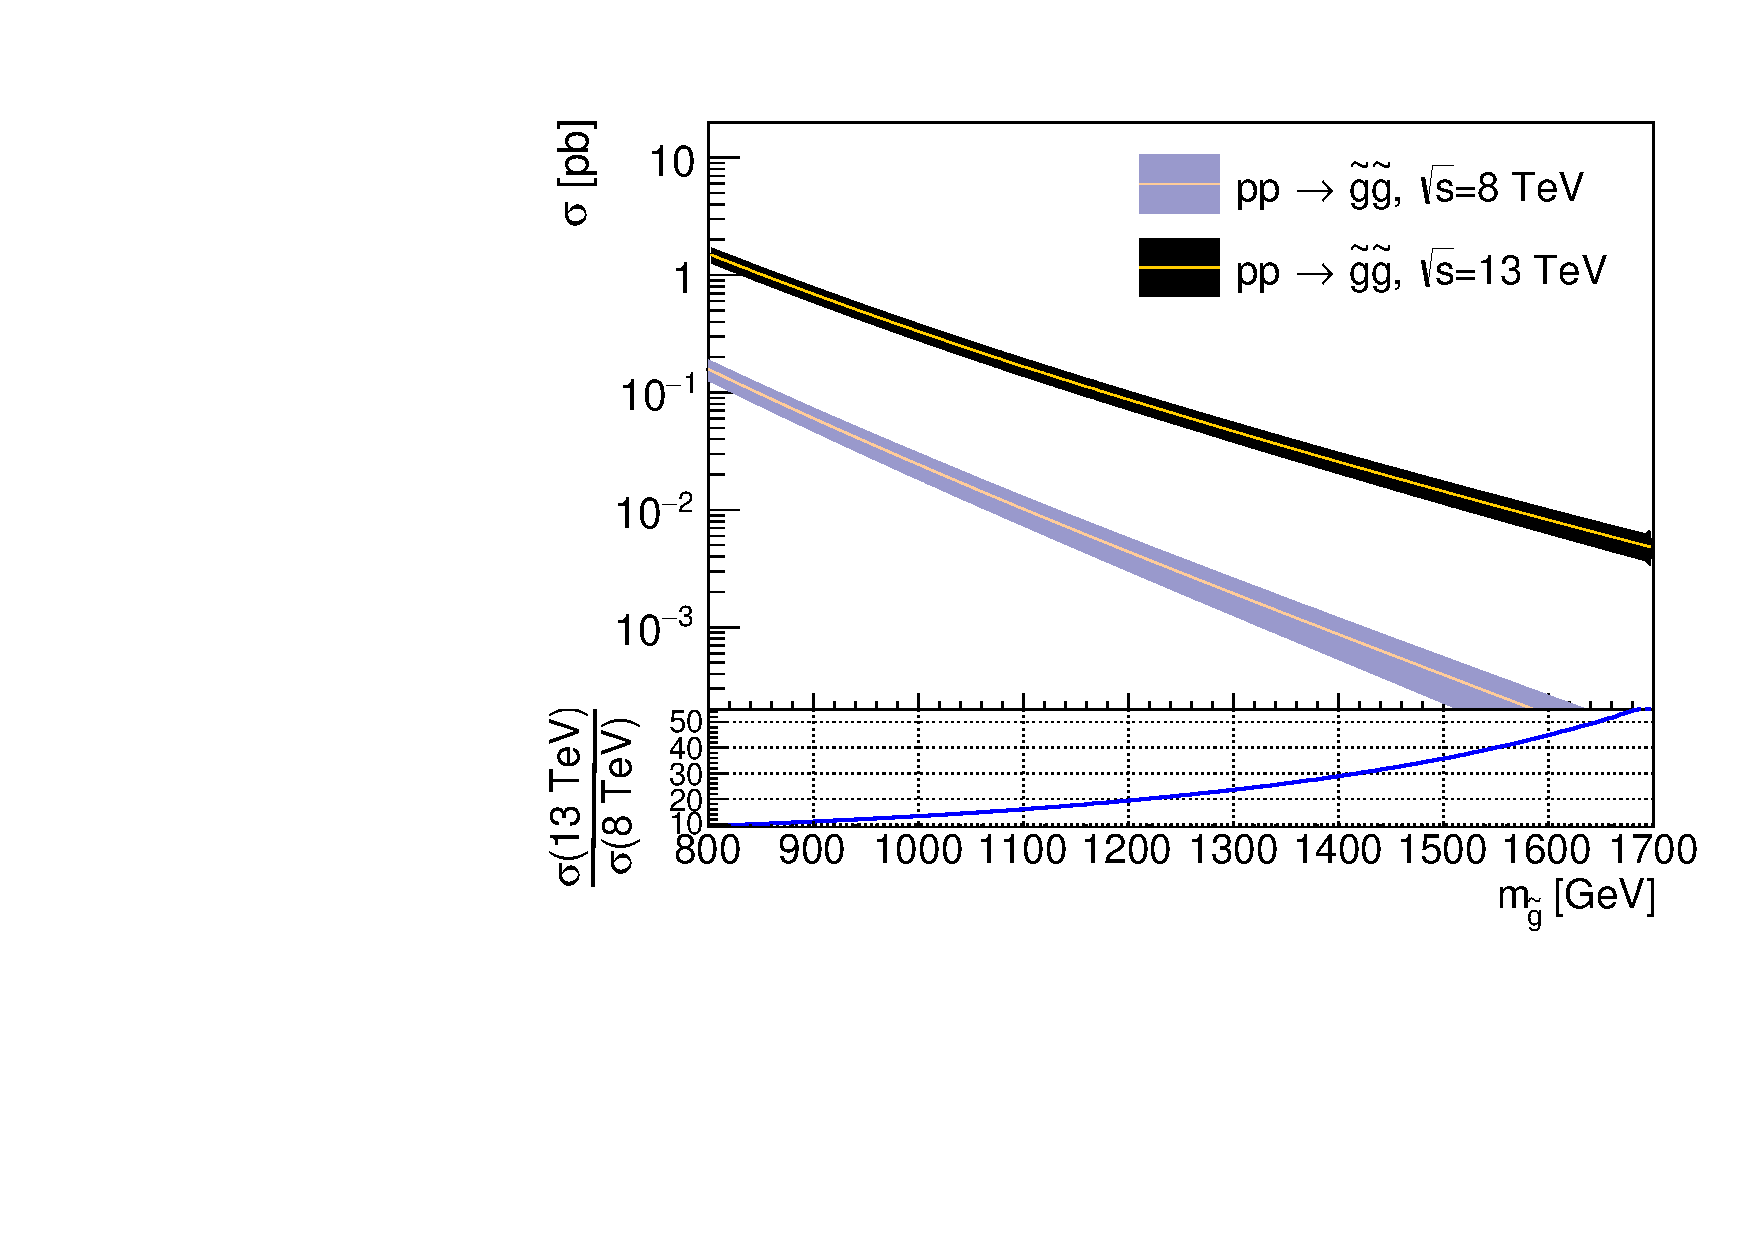
\includegraphics[width=0.45\textwidth]{figs/analysis13TeV/gluino13TeV8TeV.pdf}
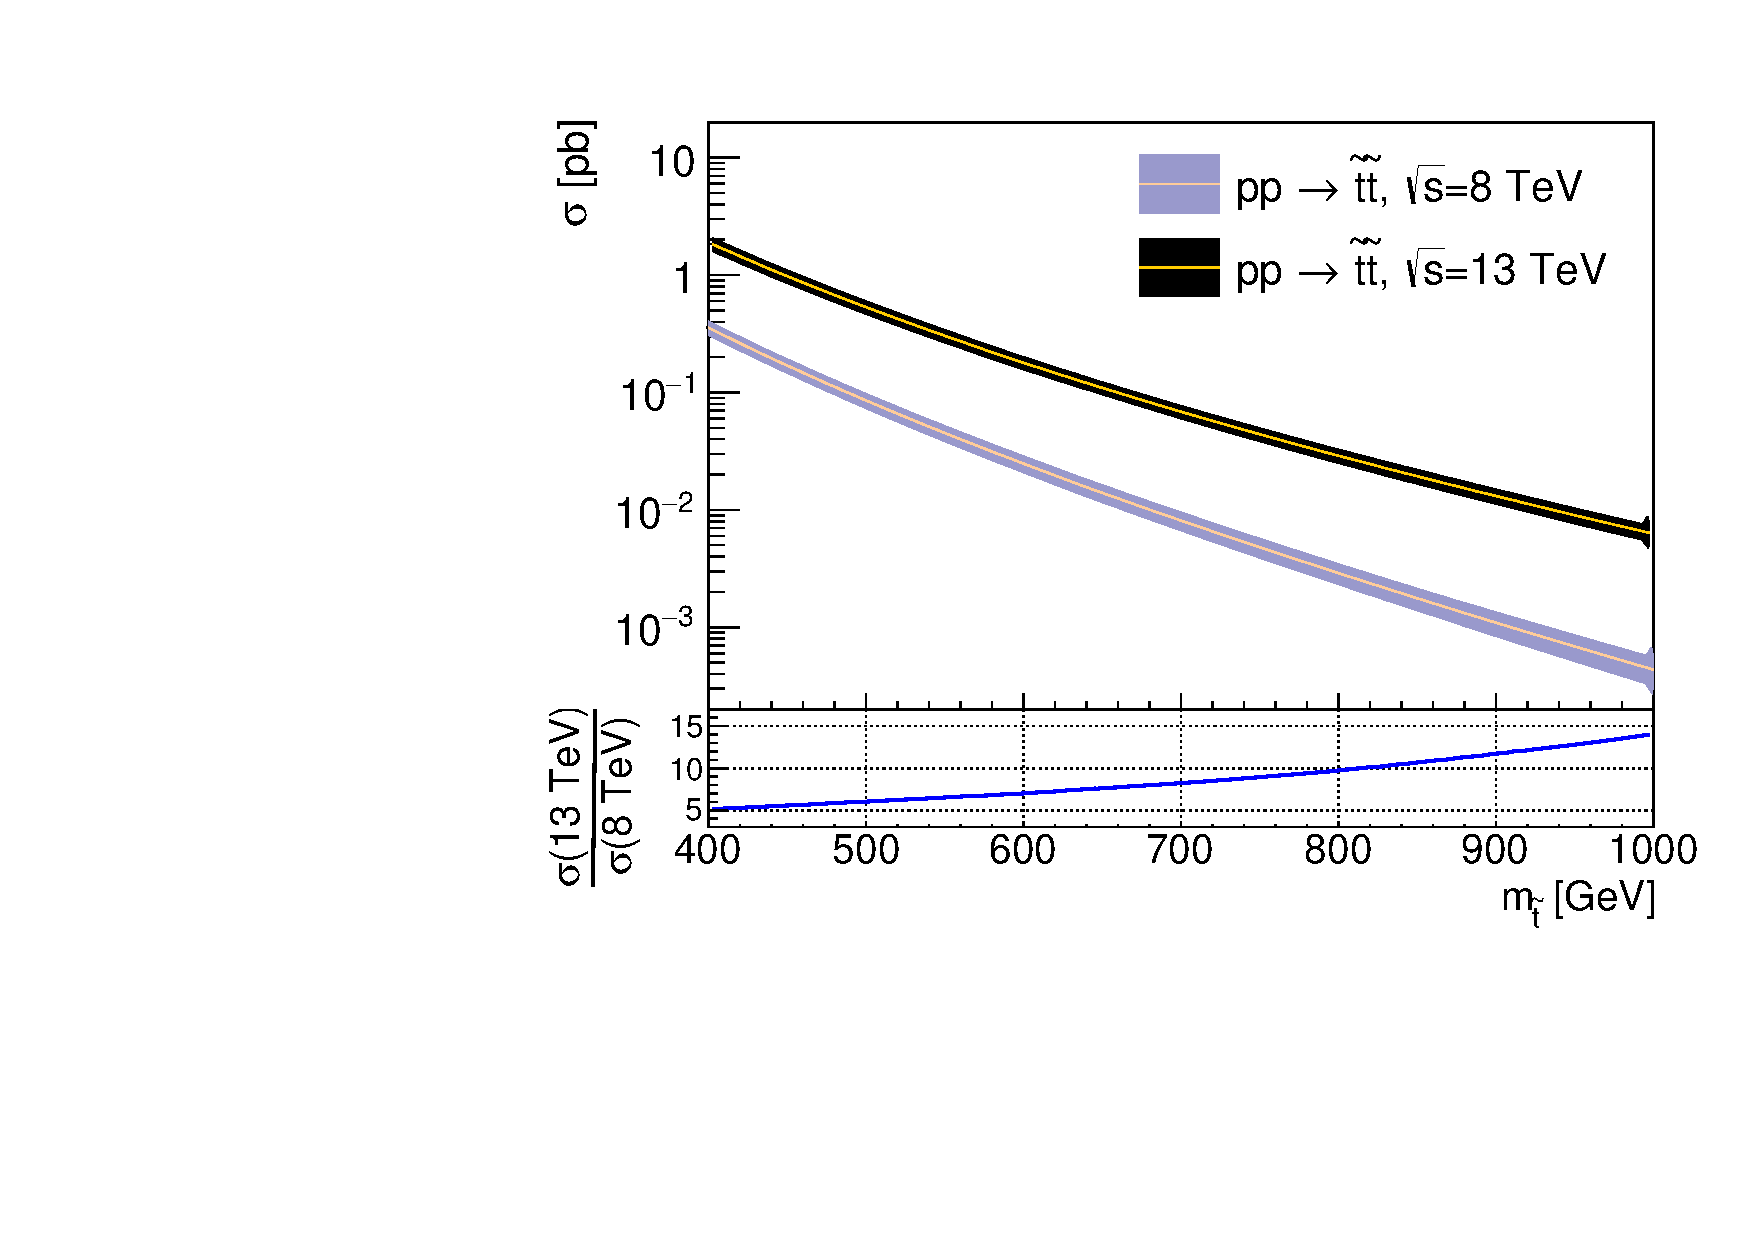
\includegraphics[width=0.45\textwidth]{figs/analysis13TeV/stop13TeV8TeV.pdf}
\caption{ The NLO$+$NLL pair production cross sections for gluinos (left) and
  top squarks (right) in $\Pp\Pp$ collisions at $\sqrt{s}=8$ and
  $13 \TeV$~\cite{NLONLL1,NLONLL2,NLONLL3,NLONLL4,NLONLL5,NLONLLerr,Borschensky:2014cia,jmgd}. The bottom panel shows the ratio of the cross sections.
 }
\label{fig:gluinostop13TeV8TeV}
\end{figure}

In this chapter, we interpret the results of the inclusive search at
13 \TeV using the simplified natural SUSY scenarios for pair production of gluinos and top
squarks detailed in Sec.~\ref{sec:sms} of this thesis. We follow a
similar strategy as the search performed at 8 \TeV, with some
changes and improvements. The modifications are the following
\begin{itemize}
\item We utilize two independent background estimation methods: one
  based on control regions in data, and assisted by the simulation,
  and one based on the fit with the empirical function.
\item Only three separate data categories -- Multijet, EleMultijet, and MuMultijet -- all of which target
  gluino production, are considered in the 13 \TeV search.
\item The anti-$\kt$ algorithm with radius parameter $R=0.4$ is used
  to cluster jets.
\item The selection of muons and electrons is updated, and in
  particular, uses a new isolation variable with a lepton $\pt$
  dependent cone size that corrects for the
  effects of pileup.
\item We reject hadronically decaying $\ensuremath{\tau}$
  leptons in the zero-lepton event categories.
\item The binned form of the maximum likelihood fit to the
  ($\MR$,$\Rtwo$) is used in all cases. 
\item The sideband region used in the model-independent search for excesses or 
    discrepancies is redefined with a tighter \MR threshold, as shown in Fig.~\ref{fig:regions13TeV}.
\item A new subcategory of events with zero \PQb-tagged jets in each category is included in the 13 \TeV search.
\item Rather than constraining the ($\MR$,$\Rtwo$) shape of $\geq3$\PQb-jet category
  category to be exactly the same as the $2$\PQb-jet category, the
  shapes of the two categories are allowed to differ with one additional nuisance
  parameter describing the deviation.
\end{itemize}
Each of these changes is described in greater detail below.

The remainder of this chapter is organized as follows. A description of simulated
signal and background samples is given in
Sec.~\ref{sec:simulation}. Sec.~\ref{sec:Objects} describes
physics object reconstruction and event
selection. Sec.~\ref{sec:StrategySelection} describes the analysis
strategy, and the background estimation techniques
used in this analysis are described in
Sec.~\ref{sec:Background}. Sec.~\ref{sec:Systematics} covers the
systematic uncertainties. Finally, our results and their interpretation
are presented in Sec.~\ref{sec:Results}, followed by a summary in Sec.~\ref{sec:Summary}. 


\section{Simulated event samples}
\label{sec:simulation}

Simulated Monte Carlo (MC) samples are used for modeling of the SM backgrounds
in the search regions and for calculating the selection efficiencies for
SUSY signal models. The production of $\ttbar+$jets, $\PW+$jets, $\cPZ+$jets, $\cPgg+$jets,
and QCD multijet events, as well as production of gluino and top squark
pairs, is simulated with the MC generator \MADGRAPH v5~\cite{Alwall:2011uj}. Single
top quark events are modeled at next-to-leading order (NLO) with \MATNLO~v2.2~\cite{Alwall:2014hca}
for the $s$-channel, and with \POWHEG~v2~\cite{Alioli:2009je, Re:2010bp}
for the $t$-channel and $\PW$-associated production. Contributions from
$\ttbar\PW$, $\ttbar\cPZ$ are also simulated with
\MATNLO~v2.2. Simulated events are interfaced with \PYTHIA
v8.2~\cite{Sjostrand2008852} for fragmentation and parton
showering.  The \textsc{NNPDF3.0LO} and \textsc{NNPDF3.0NLO}~\cite{Ball:2014uwa} parton distribution functions (PDF) are
used, respectively, with \MADGRAPH, and with \POWHEG and \MATNLO. 

The SM background events are simulated using a \GEANTfour-based model~\cite{G4} of the CMS detector.
The simulation of SUSY signal model events is performed using the CMS fast
simulation package~\cite{FastSim}. All simulated events include the
effects of pileup, i.e.~multiple $\Pp\Pp$ collisions within the same or
neighboring bunch crossings, and are processed with the same chain of
reconstruction programs as is used for collision data. Simulated events are weighted to
reproduce the observed distribution of pileup vertices in the data set, calculated based on the measured 
instantaneous luminosity. 

The SUSY signal production cross sections are calculated to next-to-leading
order (NLO) plus next-to-leading-logarithm (NLL)
accuracy~\cite{NLONLL1,NLONLL2,NLONLL3,NLONLL4,NLONLL5,NLONLLerr,Borschensky:2014cia}, assuming all
SUSY particles other than those in the relevant diagram to be too
heavy to participate in the interaction. The NLO$+$NLL cross section and
its associated uncertainty~\cite{Borschensky:2014cia} are used to derive 
the exclusion limit on the masses of the SUSY
particles. The hard scattering was generated with \MADGRAPH up to
two extra partons to model initial-state radiation at the matrix element level, and
simulated events were interfaced to  \PYTHIA for the showering,
fragmentation and hadronization steps. 

\section{Object reconstruction and selection}
\label{sec:Objects}
Physics objects are defined using the particle-flow (PF)
algorithm~\cite{PF1,PF2}, described in Sec.~\ref{sec:pf}. The reconstructed PF candidates are clustered into jets using the 
anti-$k_\mathrm{t}$ algorithm~\cite{antikt, fastjet}
with a distance parameter of $0.4$ for 13\TeV instead of $0.5$ used at
8 \TeV. 
%The jet momentum is determined as the vector sum of all particle momenta
%in the jet, and jet-energy corrections are derived from simulation and
%confirmed by in-situ measurements of the energy balance in dijet
%and $\Pgg+$jet events. Jets are required to pass loose identification criteria 
%on the jet composition designed to reject spurious signals arising from noise and 
%failures in the event reconstruction~\cite{CMS-PAS-JME-10-003, Khachatryan:2016kdb}.
As in the 8 \TeV search, we consider jets with transverse momentum $\pt>40\GeV$ and
$|\eta|<3.0$. 
%The missing transverse momentum vector \ptvecmiss
%is defined as the projection on the plane perpendicular to the beams of
%the negative vector sum of the momenta of all reconstructed  PF
%candidates in an event. Its magnitude is referred to as the missing
%transverse energy \ETmiss.
 

Electrons are reconstructed by associating a cluster of
energy deposited in the ECAL with a reconstructed track~\cite{Khachatryan:2015hwa}, 
and are required to have $\pt > 5 \GeV$ and $|\eta|<2.5$. A ``tight'' selection
used to identify prompt electrons is based on requirements
on the electromagnetic shower shape, the geometric matching of
the track to the calorimeter cluster, the track quality and impact
parameter, and isolation. The isolation of electrons and muons is
defined as the scalar sum of the transverse momenta of all neutral and
charged PF candidates within a cone $\Delta R = \sqrt{(\Delta\eta)^2+(\Delta\phi)^2}$ along the lepton
direction. The variable is corrected for the effects of pileup using an
effective area correction~\cite{CMS-PAS-JME-14-001}, and the cone size
$\Delta R$ shrinks with increasing lepton $\pt$  according to
\begin{equation}
 \label{eq:miniIsolation}
 \Delta R= 
 \begin{cases}
 0.2, & \pt \le 50\ \GeV\\
 \frac{10 \GeV}{\pt}, & 50\ < \pt \le 200\ \GeV \\
 0.05, & \pt > 200\ \GeV. \\
\end{cases}
 \end{equation}
The use of the lepton $\pt$ dependent isolation cone enhances the
efficiency of identifying leptons in events containing a large amount of hadronic
energy, such as those with $\ttbar$ production. For tight electrons, the isolation is required to be less than $10\%$ of 
the electron $\pt$. The selection efficiency for tight electrons increases from $60\%$ for $\pt$ around $20\GeV$
to $70\%$ for $\pt$ around $40\GeV$ and to $80\%$ for $\pt$ above
$50\GeV$. 

To improve the purity of all-hadronic signals in the zero-lepton event categories, a looser ``veto''
selection is also defined.  For this selection, electrons are required to have $\pt>5 \GeV$.  The output of a boosted decision tree is used to identify electrons based on shower
shape and track information~\cite{Khachatryan:2015hwa}.  
For electrons with $\pt>20 \GeV$, the isolation is required to be less than $20\%$ of the 
electron $\pt$.  For electrons with $\pt$ between $5$ and $20 \GeV$, the value of the 
absolute isolation, computed by summing the $\pt$'s of all particle flow candidates within a 
$\Delta R$ cone of $0.3$, is required to be less than $5 \GeV$. For
the veto electron selection, the efficiency increases from $60\%$ for
$\pt$ around $5 \GeV$ to $80\%$ for $\pt$ around $15 \GeV$ and $90\%$ for $\pt$ above $20 \GeV$. 

Muons are reconstructed by combining tracks found in the muon system with 
corresponding tracks in the silicon detectors~\cite{Chatrchyan:2012xi},
and are required to have $\pt > 5 \GeV$ and $|\eta|<2.4$. Muons are identified
based on the quality of the track fit, the number of detector hits used in the 
tracking algorithm, and the compatibility between track
segments. As for electrons, we define ``tight'' and ``veto'' muon selections. The absolute value of the 3D impact 
parameter significance of the muon track, which is defined as the ratio of the impact
parameter to its estimated uncertainty, is required to be less than
4. For both tight and veto muons with 
$\pt > 20 \GeV$ the isolation is required to be less than $20\%$
of the muon $\pt$, while for veto muons with $\pt$ between $5$ and $20 \GeV$
the isolation computed using a $\Delta R$ cone of $0.4$ 
is required to be less than $10 \GeV$. For tight muons we require $d_0<0.2 \unit{cm}$, where $d_0$ is the transverse impact parameter of the muon
track, while this selection is not applied for veto muons. 
The selection efficiency for tight muons increases from $65\%$ for
$\pt$ around $20 \GeV$ to $75\%$ for $\pt$ around 40~$\GeV$ and to $80\%$ for $\pt$ above $50 \GeV$. 
For the veto muon selection, the efficiency increases from $85\%$ for
$\pt$ around $5 \GeV$ to $95\%$ for $\pt$ above 20~$\GeV$. 

We additionally reconstruct and identify hadronically decaying $\ensuremath{\tau}$ 
leptons ($\ensuremath{\tau_{\mathrm{h}}}$) to further enhance the all-hadronic purity 
of the zero-lepton event categories, using the hadron-plus-strips algorithm~\cite{Khachatryan:2015dfa}, which
identifies $\ensuremath{\tau}$ decay modes
with one charged hadron and up to two neutral pions, or three charged hadrons.
The $\ensuremath{\tau_{\mathrm{h}}}$ candidate is required to have
$\pt>20 \GeV$, and the isolation, defined as the $\pt$ sum of other nearby PF candidates, must be below a certain threshold. 
The loose cutoff-based selection~\cite{Khachatryan:2015dfa} is used and results in an efficiency
of about $50\%$ for successfully reconstructed $\ensuremath{\tau_{\mathrm{h}}}$ decays.

To identify jets originating from \cPqb-hadron decays, we use the updated
CSVv2 \cPqb-jet tagger (see Sec.~\ref{sec:btag}), which uses the inclusive
vertex finder to select \cPqb-jets~\cite{CMS-PAS-BTV-15-001,btag8TeV,btag7TeV}. The ``medium'' 
working point selection is used to define the event categories for the search signal regions,
and for jets with $\pt$ between $40$ and $200 \GeV$ yields an
efficiency of approximately $70\%$ for \cPqb-jets and an average 
misidentification probability of $1.5\%$ for jets originating from light-flavor 
quarks or gluons in typical background events relevant for this search.

Photon candidates are reconstructed from clusters of energy deposits
in the ECAL. They are identified using selections on the hadronic to
electromagnetic energy ratio ($H/E$) and the transverse shower width $\sigma_{\eta\eta}$,
measured in terms of the energy weighted spread within the $5\times 5$ crystal matrix centered on the crystal with the largest energy deposit in the supercluster~\cite{CMSPhoton},
\begin{equation}
(\sigma_{\eta\eta})^2 = \frac{\left ( \sum_{5\times 5} (\eta_i -
    \bar\eta)^2w_i\right )}{\sum_{5\times 5} w_i}~,
\end{equation}
where $w_i$ is a weight that depends logarithmically on the energy.
Photon isolation, defined as the scalar $\pt$ sum of charged particles within a cone of
$\Delta R<0.3$, must be less than $2.5 \GeV$. Finally, photon candidates that share
the same energy cluster as an identified electron are vetoed. 

\section{Analysis strategy and event selection}
\label{sec:StrategySelection}

We employ an event classification approach similar to the one used in the 8\TeV
search in Sec.~\ref{sec:box8TeV}. We select events with four or more jets, using search categories
defined by the number of leptons and \cPqb-tagged jets in the event. 
Events in the zero lepton category, denoted as the Multijet category, are required to have no 
electrons or muons passing the tight or veto selection, and no selected $\ensuremath{\tau_{\mathrm{h}}}$. 
The Multijet category consists of events with no electrons or muons passing the tight or veto selection, and no selected $\ensuremath{\tau_{\mathrm{h}}}$. 
Events in the one electron (muon) category, denoted as the Electron Multijet (Muon Multijet) category,
are required to have one and only one electron (muon) passing the tight selection.
Within these three event classes, we divide the events further into categories depending on
whether the events have zero, one, two, or more than two \cPqb-tagged jets. 

Each event in the above categories is treated as a dijet-like event by grouping selected leptons 
and jets in the event into two megajets in order to compute the razor variables $\MR$  and $\Rtwo$ defined
in Sec.~\ref{sec:kinematic}. 

The events of interest are triggered either by the presence of a high-$\pt$ electron or muon, or 
through dedicated hadronic triggers requiring the presence of at least two highly energetic jets 
and with loose thresholds on the razor variables $\MR$ and $\Rtwo$. The single-electron (single-muon) triggers require at least one isolated electron 
(muon) with $\pt>23$ ($20$)~$\GeV$. The isolation requirement is dropped for electrons (muons) with 
$\pt>105$ ($50$)~$\GeV$. The efficiencies for the single electron (muon) triggers
are above $70$\% for $\pt$ around $25$ ($20$)~$\GeV$, and reach a
plateau above $97$\% for $\pt>40 \GeV$. The efficiencies for the single electron trigger were measured in data and simulation and
found to be in good agreement, as were the corresponding efficiencies for muons. Corrections for residual difference of trigger
efficiency  between data and MC simulation are applied to simulated samples.
The hadronic razor trigger requires at least two jets with $\pt > 80 \GeV$ or at least 
four jets with $\pt > 40 \GeV$. The events are also required to pass selections on the 
razor variables $\MR>200\GeV$ and $\Rtwo>0.09$ and on the product 
$(\MR + 300 \GeV)\times(\Rtwo + 0.25)>240 \GeV$.
The efficiency of the hadronic razor trigger for events passing the baseline
$\MR$ and $\Rtwo$ selections described below is $97\%$ and is consistent
with the prediction from MC simulation.

For events in the Electron or Muon Multijet categories, the search region 
is defined by the selections $\MR > 400 \GeV$ and $\Rtwo > 0.15$. 
The $\pt$ of the electron (muon)
is required to be larger than $25$ ($20 \GeV$). To suppress backgrounds from the $\PW(\ell\nu)+$jets
and $\ttbar$ processes, we require that the transverse mass $M_{\mathrm{T}}$ formed by the lepton
and \ptvecmiss be larger than $120 \GeV$. 

For events in the Multijet category, the search uses a region defined by the 
selections $\MR > 500 \GeV$ and $\Rtwo > 0.25$ and requires the presence of at least 
two jets with $\pt >80 \GeV$ within $|\eta|<3.0$, for compatibility with the requirements 
imposed by the hadronic razor triggers. For QCD multijet background events, the
\ETmiss arises mainly from mismeasurement of
the energy of one of the leading jets.  In such cases, the two razor 
megajets tend to lie in a back-to-back configuration. Therefore, to suppress the QCD multijet 
background we require that the azimuthal angle $\dPhiR$ between the two razor
megajets be less than $2.8$ radians. 

Finally, events containing signatures consistent with beam-induced background or anomalous noise 
in the calorimeters are rejected using dedicated 
filters~\cite{Chatrchyan:2011tn,Khachatryan:2014gga}.

\section{Background modeling}
\label{sec:Background}

The main background processes in the search regions considered are
$\PW(\ell\nu)+$jets (with $\ell=\Pe,\Pgm,\ensuremath{\tau}$), $\cPZ(\nu\bar\nu)+$jets, $\ttbar$, and QCD multijet production. For event categories with
zero \PQb-tagged jets, the background is primarily composed of the $\PW(\ell\nu)+$jets and $\cPZ(\nu\bar\nu)+$jets
processes, while for categories with two or more \PQb-tagged jets it is
dominated by the $\ttbar$ process. There are also very small contributions from
the production of two ($\cPV\cPV$) or three electroweak bosons
($\cPV\cPV\cPV$) and from the production of $\ttbar$ in
association with a $\PW$ or $\cPZ$ boson ($\ttbar\cPV$). These
contributions are summed and labeled ``Other'' in Fig.~\ref{fig:TTBarWJetsCR_MR}-\ref{fig:Znn_PhotonJets}.

We model the background using two independent methods based on control samples in data with entirely
independent sets of systematic assumptions. The first method (A) is based on the use of 
dedicated control regions that isolate a specific background processes in order 
to control and correct the predictions of the MC simulation. 
The second method (B) is based on a fit to an assumed functional 
form for the shape of the observed data distribution in the
two-dimensional ($\MR$,$\Rtwo$) plane as in the 8 \TeV search.
These two background predictions are compared to and cross-checked against each other in order 
to significantly enhance the robustness of the background estimate. 


\subsection{Method A: simulation-assisted background prediction}
\label{sec:MADD}

The simulation-assisted method defines dedicated control regions that isolate
each of the main background processes. Data in these control regions are used 
to control and correct the accuracy of the MC prediction for each of the
background processes. Corrections for the jet energy response and lepton momentum response
are applied to the MC, as are corrections for the trigger 
efficiency and the selection efficiency of electrons, muons, and \PQb-tagged jets. Any
disagreement observed in these control regions is then interpreted as an inaccuracy of the 
MC in predicting the hadronic recoil spectrum and jet multiplicity. 

Two alternative formulations of the method are typically used in searches for
new physics~\cite{SUS12024,MT2at8TeV,Aad:2013wta}. 
In the first formulation, the data control region yields are extrapolated to the search regions
via translation factors derived from simulation.  In the second formulation, simulation to data 
correction factors are derived in bins of the razor variables $\MR$ and $\Rtwo$ 
and are then applied to the simulation prediction of the search region yields. 
The two formulations are identical and the choice of which formulation is used  
depends primarily on the convenience of the given data processing sequence. 
In both cases, the contributions from background processes other than the one
under study are subtracted using the MC prediction.
We employ the first formulation of the method for the estimate of the QCD background, 
while the second formulation is used for modeling all other major backgrounds. 
Details of the control regions used for each of 
the dominant background processes are described in the subsections below.

Finally, the small contribution from rare background processes such as $\ttbar\cPV$ is
modeled using simulation. Systematic uncertainties on the cross sections of these processes
are propagated to the final result. 

\subsubsection{The $\ttbar$ and $\PW(\ell\nu)+$jets background}
\label{sec:TTBarWJetsCR}

The control region to isolate the $\ttbar$ and $\PW(\ell\nu)+$jets processes is defined by requiring 
at least one tight electron or muon. To suppress QCD multijet
background, the quantities \ETmiss and $M_{\mathrm{T}}$ are both required to be larger than $30 \GeV$. To minimize 
contamination from potential SUSY processes and to explicitly separate the control region
from the search regions, we require $M_{\mathrm{T}} < 100 \GeV$. The $\ttbar$ enhanced control region is defined by requiring that there be at 
least one \PQb-tagged jet, and the $\PW(\ell\nu)+$jets enhanced control region is defined by
requiring no such \PQb-tagged jets. Other than these  \PQb-tagged jet
requirements, we place no explicit requirement on the number of jets in
the event, in order to benefit from significantly larger control samples. 

We first derive corrections for the $\ttbar$ background, and then measure
corrections for the $W(\ell\nu)+$jets process after first applying the corrections already obtained
for the $\ttbar$ background in the $W(\ell\nu)+$jets control region.
As discussed above, the corrections to the MC prediction are derived in two-dimensional bins of the
($\MR$,$\Rtwo$) plane. We observe that the $\MR$ spectrum predicted by the simulation
falls off more steeply than the control region data for both the $\ttbar$ and $\PW(\ell\nu)+$jets
processes, as shown in Fig.~\ref{fig:TTBarWJetsCR_MR}. 
In Fig.~\ref{fig:WJets_TTBarDileptonCR_MRRsqUnrolled}, we show the two-dimensional ($\MR$,$\Rtwo$) distributions
for data and simulation in the $\PW(\ell\nu)+$jets control region. The statistical uncertainties in the correction factors
due to limited event yields in the control region bins are propagated and dominate the total uncertainty 
of the background prediction. For bins at large $\MR$ (near $1000\GeV$), the statistical uncertainties 
range between $15\%$ and $50\%$. 

\begin{figure}[!ptb] \centering
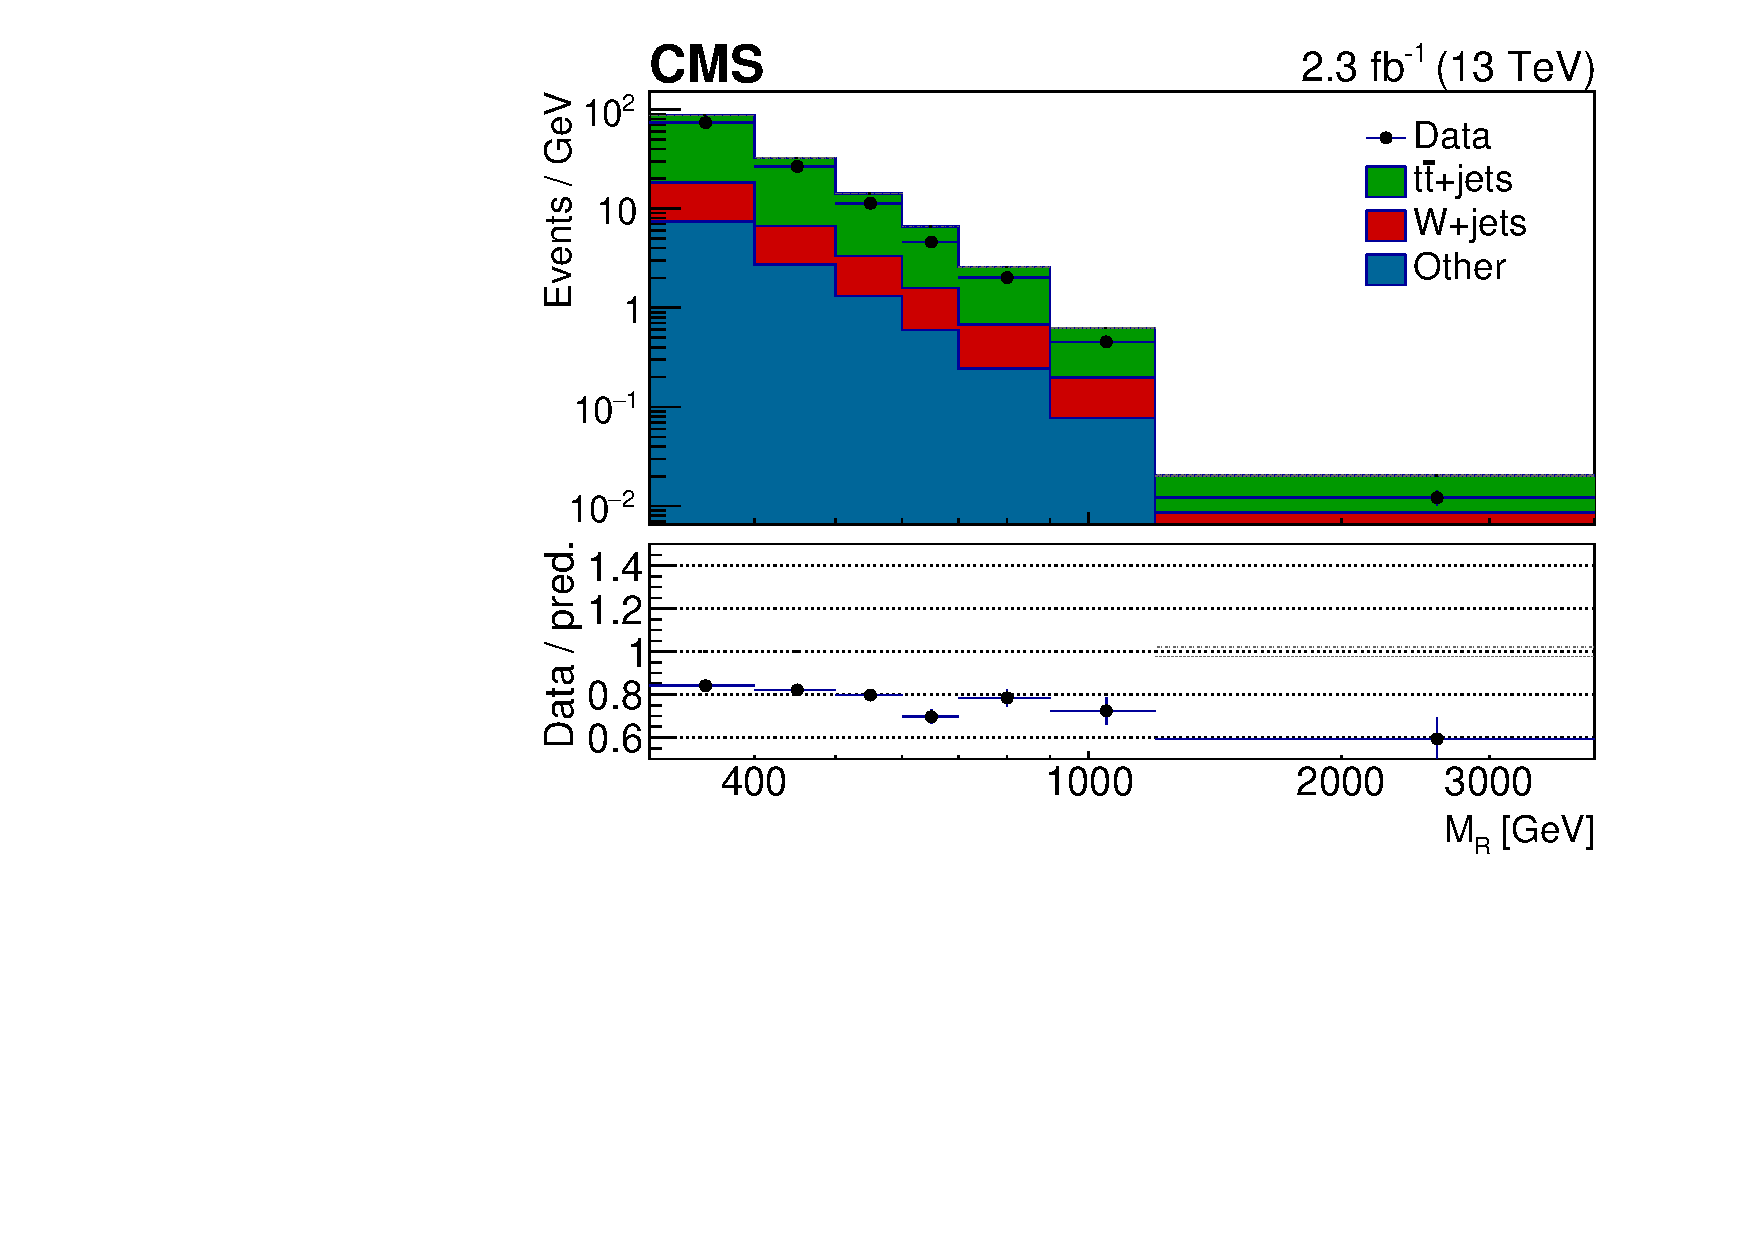
\includegraphics[width=0.45\textwidth]{figs/analysis13TeV/TTBarWJets/MR_TTJetsSingleLepton.pdf}
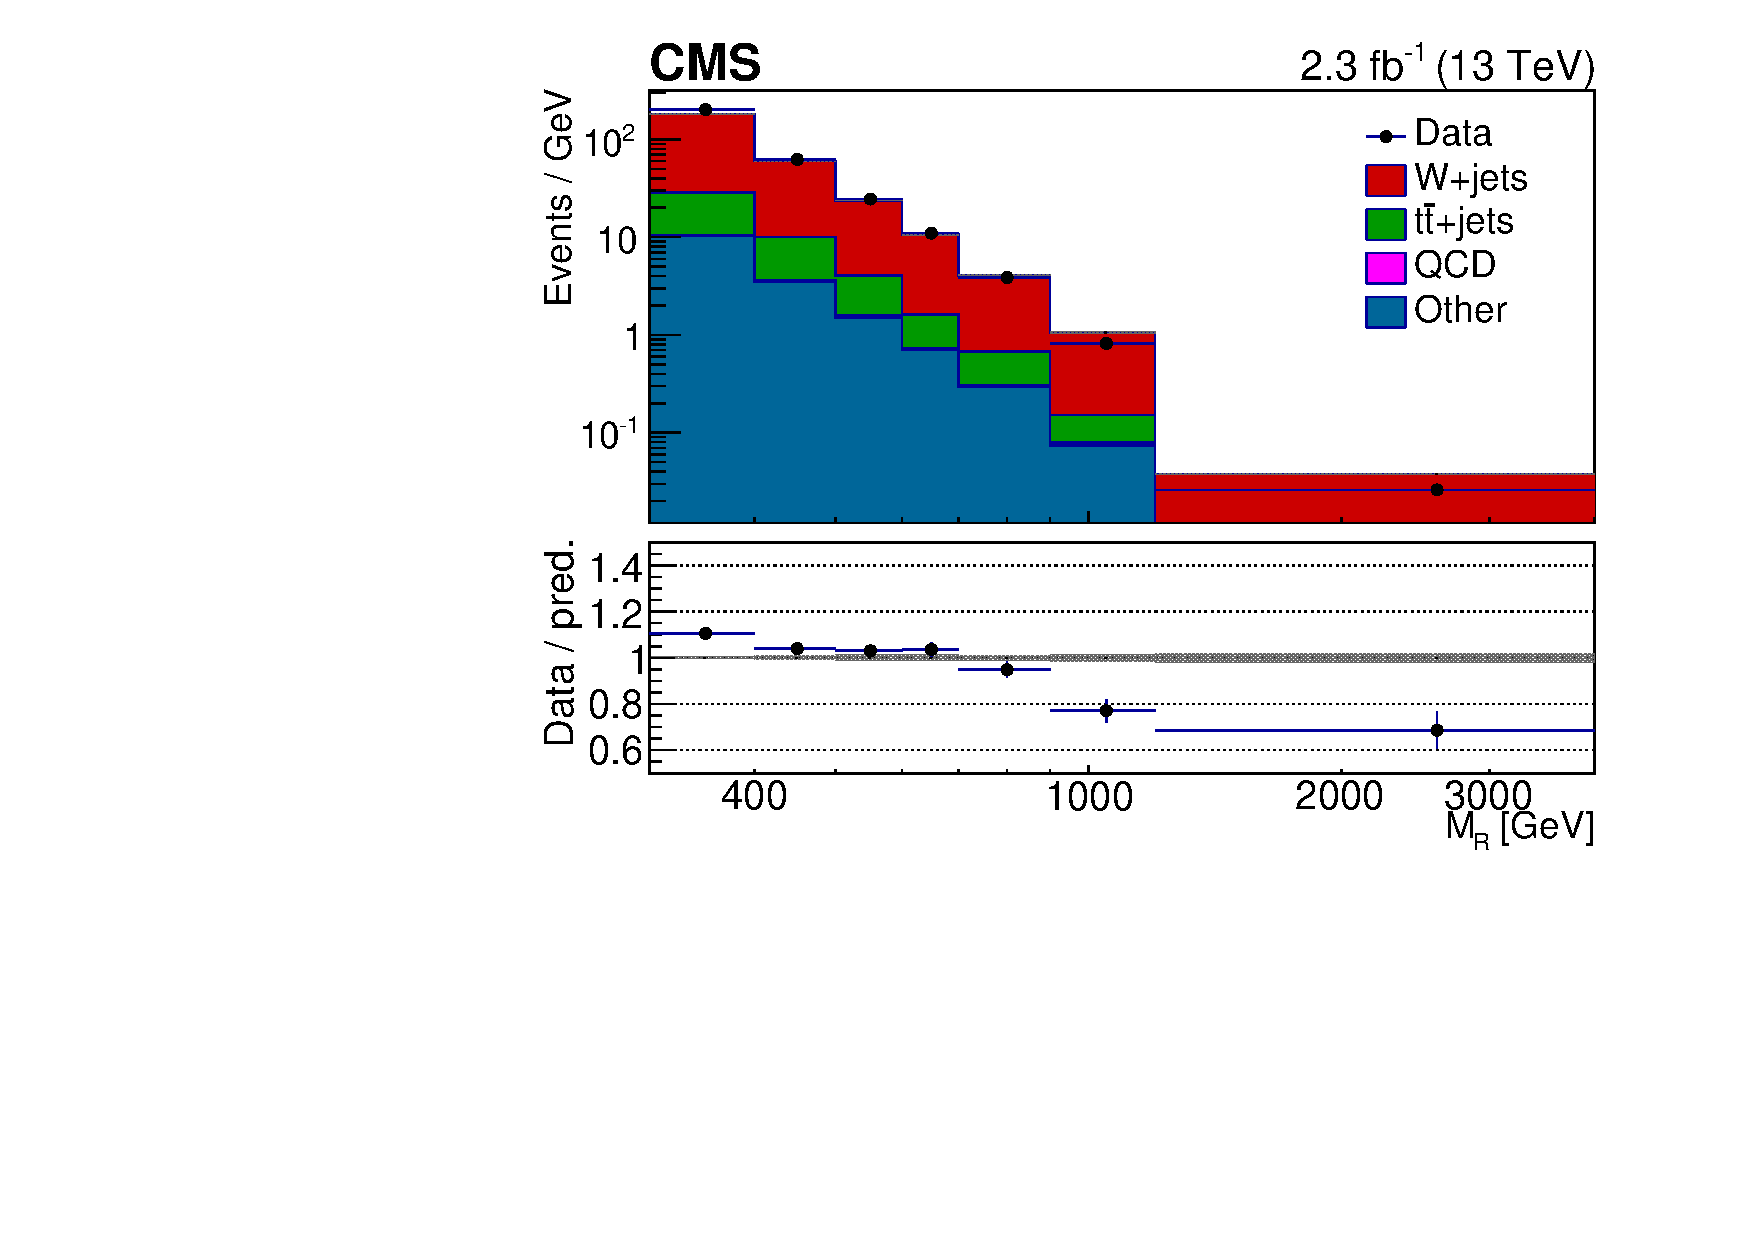
\includegraphics[width=0.45\textwidth]{figs/analysis13TeV/TTBarWJets/MR_WJetsSingleLepton.pdf}
\caption{ The $\MR$ distributions for events in the $\ttbar$ (left) and $\PW(\ell\nu)$+jets (right) 
control regions are shown, comparing data with the MC prediction~\cite{CMS-PAS-SUS-15-004}.  
The ratio of data to the background prediction is shown on the bottom panel,
with the statistical uncertainty expressed through the data point error bars and the 
systematic uncertainty of the background prediction represented by the shaded region.
In the right-hand plot, the $\ttbar$ MC events have been reweighted
according to the corrections derived in the $\ttbar$-enhanced control
region.
 }
\label{fig:TTBarWJetsCR_MR}
\end{figure}

\begin{figure}[!ptb] \centering
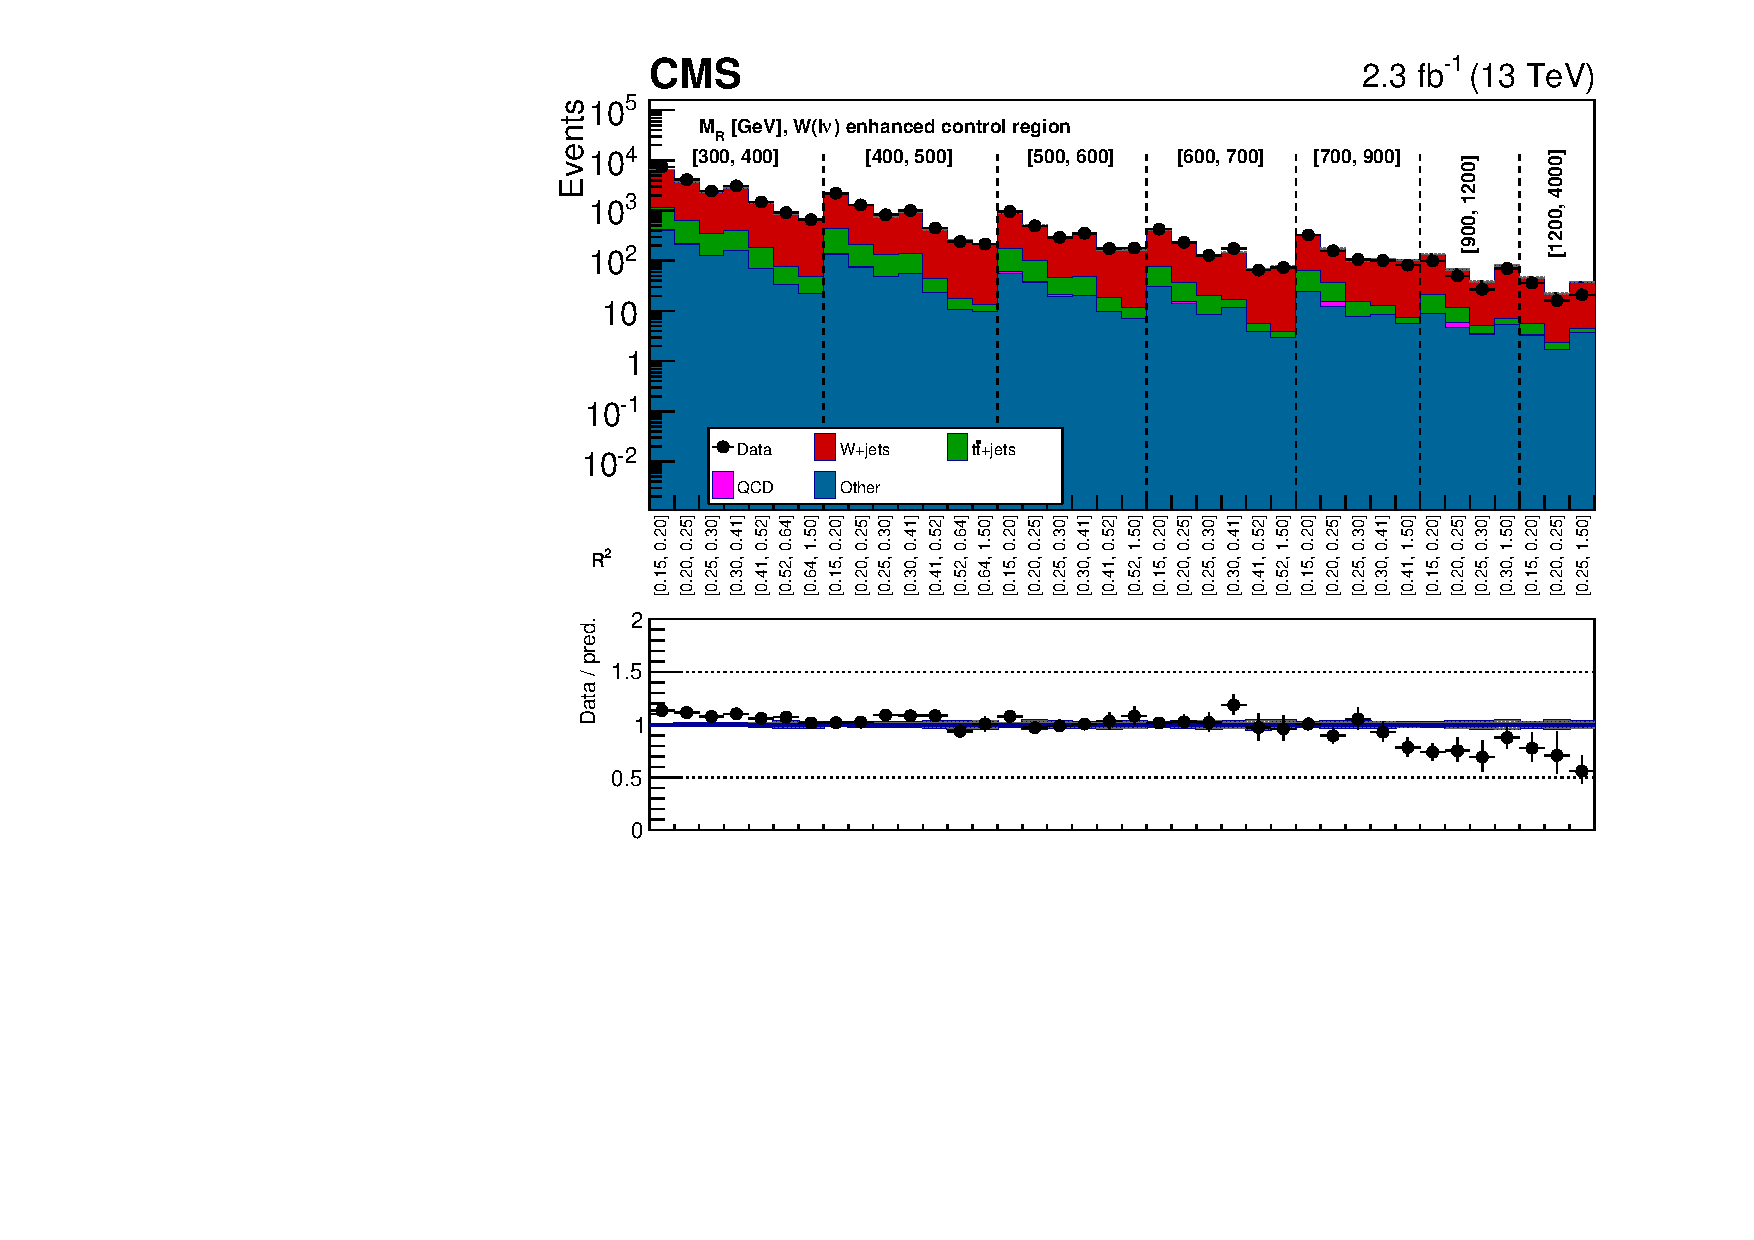
\includegraphics[width=0.95\textwidth]{figs/analysis13TeV/TTBarWJets/MRRsqWJetsSingleLeptonUnrolledDataMC.pdf}
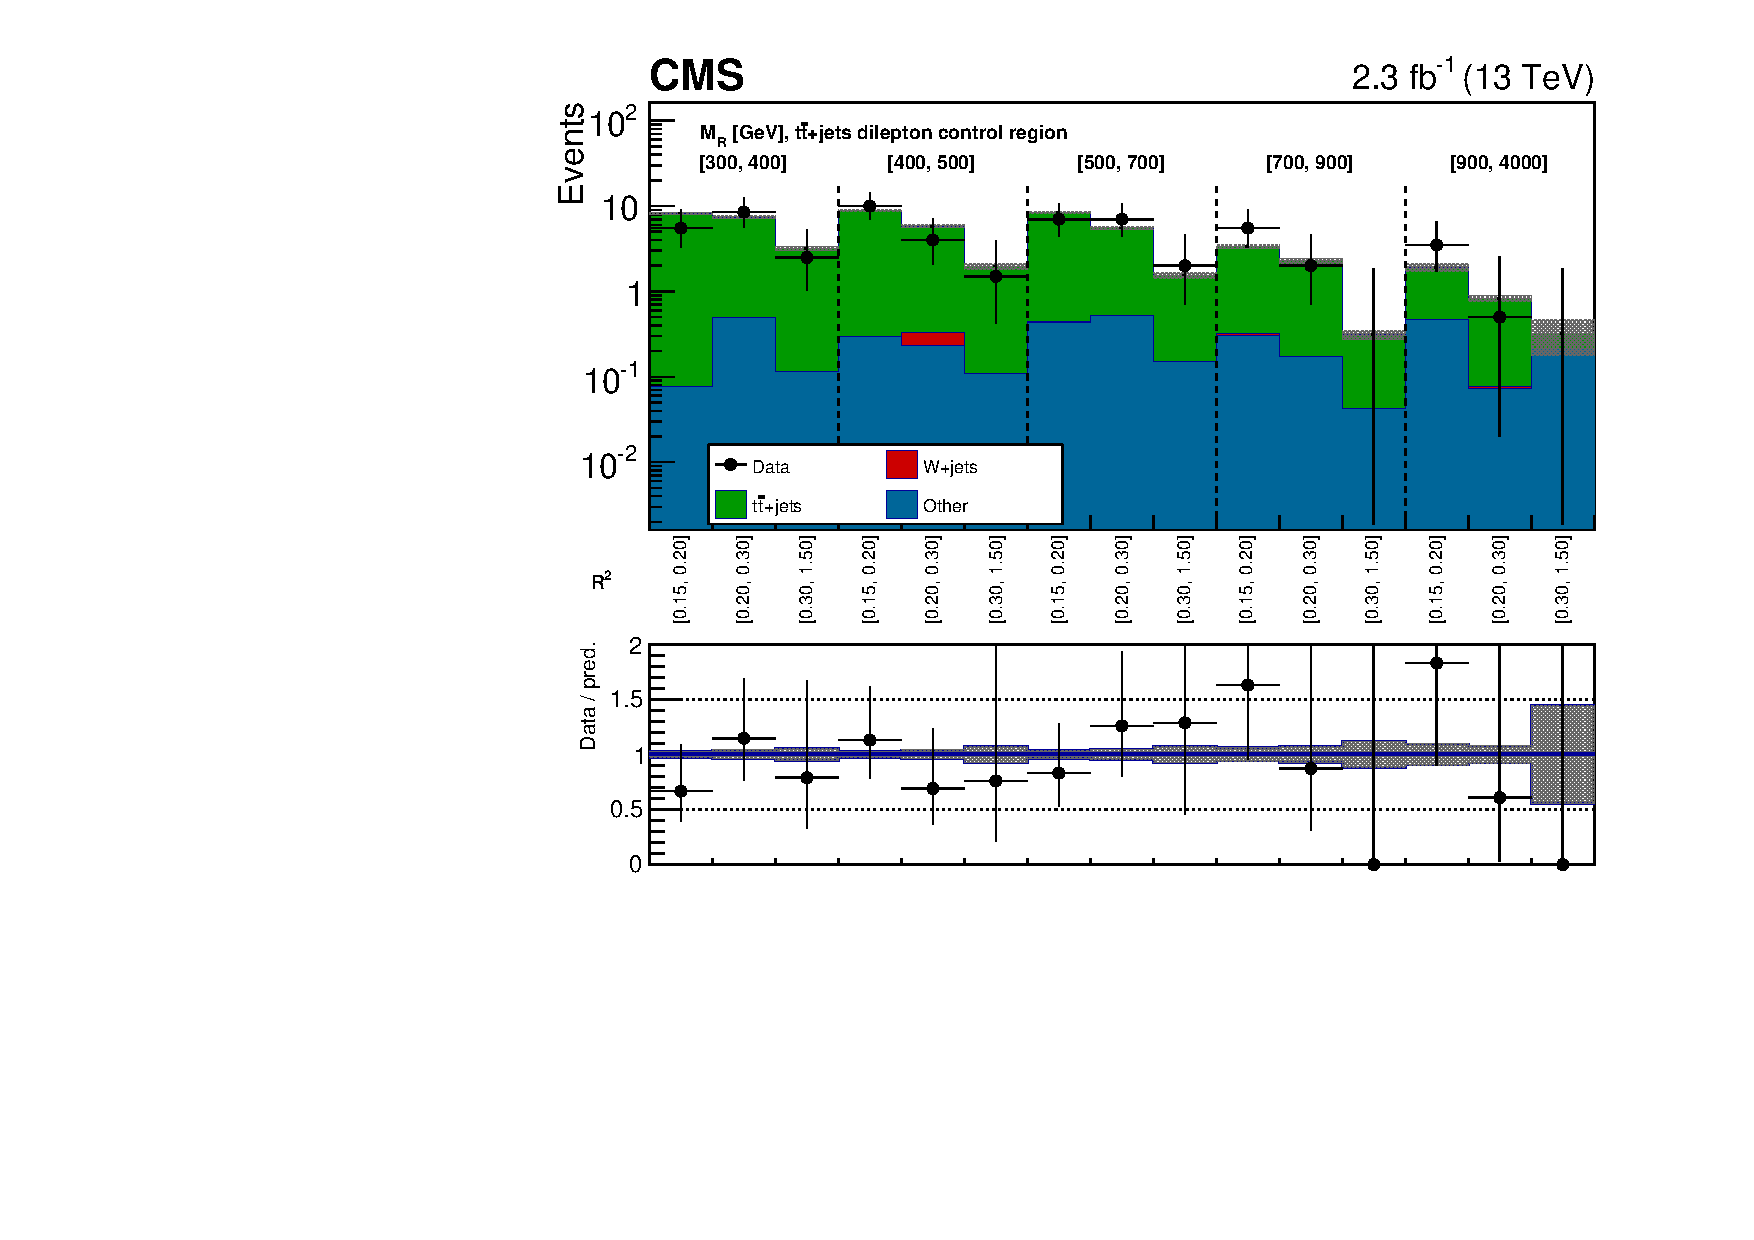
\includegraphics[width=0.95\textwidth]{figs/analysis13TeV/TTBarWJets/Razor_TTBarDileptonCrossCheckRegion_MRRsqUnrolled_MR300Rsq0p15_all_Logy.pdf}
\caption{The two-dimensional $\MR$-$\Rtwo$ distribution for the
  $\PW(\ell\nu)$+jets enhanced (upper) and the $\ttbar$ dilepton (lower)
  control regions are shown, comparing data with the MC prediction~\cite{CMS-PAS-SUS-15-004}. The $\ttbar$ MC events have been reweighted according to the correction factors
derived in the $\ttbar$-enhanced control region.  The two-dimensional $\MR$-$\Rtwo$ distribution is shown
in a one dimensional representation, with each $\MR$ bin marked by the dashed lines and labeled near the top
, and each $\Rtwo$ bin labeled below. 
The bottom panel shows the ratio of data to the background prediction, with uncertainties displayed as in Fig.~\ref{fig:TTBarWJetsCR_MR}.
}
\label{fig:WJets_TTBarDileptonCR_MRRsqUnrolled}
\end{figure}

% \begin{figure}[!htb] \centering
% 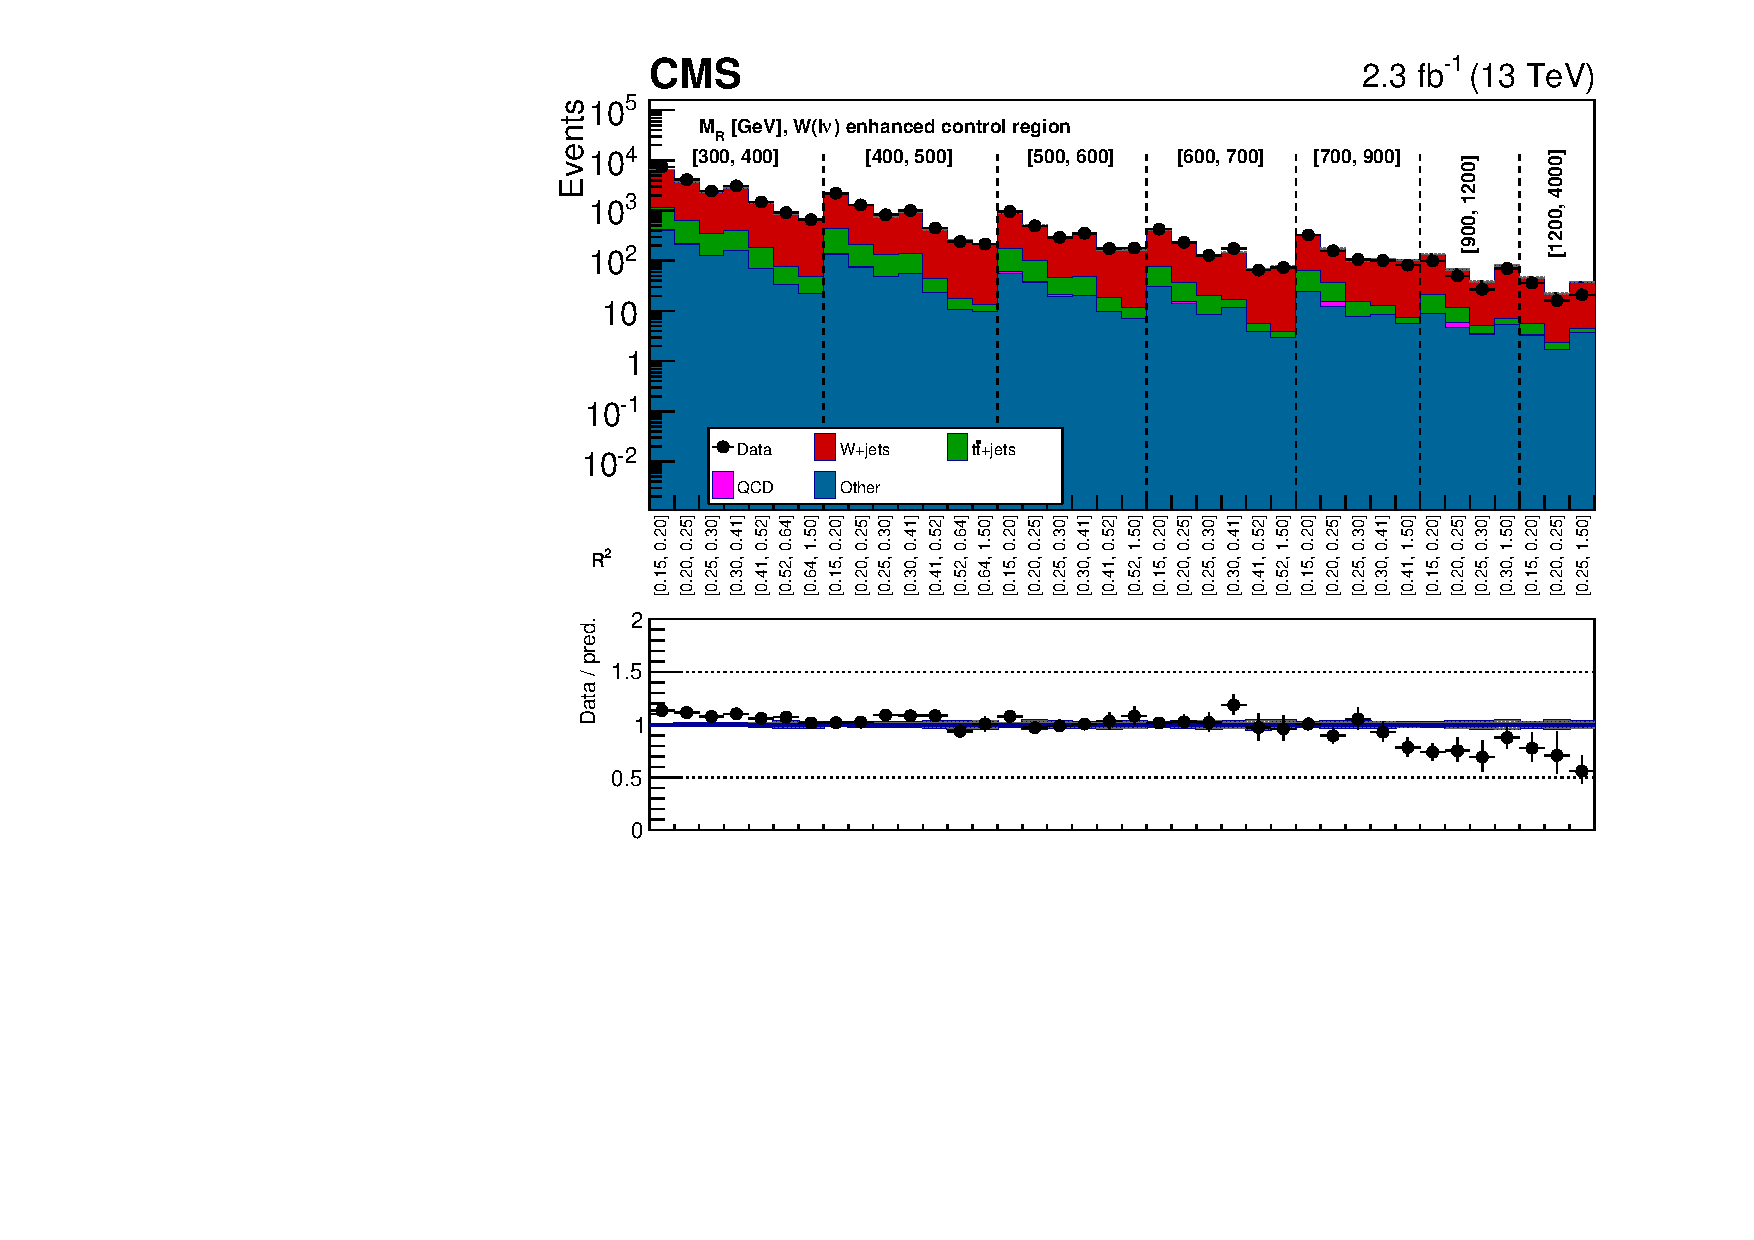
\includegraphics[width=0.95\textwidth]{figs/analysis13TeV/TTBarWJets/MRRsqWJetsSingleLeptonUnrolledDataMC.pdf}
% \caption{ The two dimensional $\MR-\Rtwo$ distribution for the $\PW(\ell\nu)+$jets enhanced control region 
% is shown, comparing data with the MC prediction. The $\ttbar$ MC events in this control sample have been reweighted 
% according to the corrections derived in the $\ttbar$ enhanced control region. The two-dimensional ($\MR$,$\Rtwo$) 
% distribution is shown in a one dimensional representation, with each $\MR$ bin marked by the dashed lines and labeled near the top,
% and each $\Rtwo$ bin labeled below. The ratio of data to the background prediction is shown in the bottom inset, with
% the statistical uncertainty expressed through the data point error bars and the systematic uncertainty in the
% background prediction represented by the shaded region. 
% }
% \label{fig:WJetsControlRegion_MRRsq_Unrolled}
% \end{figure}

Corrections to the MC simulation are first measured and applied as a function of $\MR$ and $\Rtwo$, inclusively in the
number of selected jets. As our search region requires a higher multiplicity of jets, an additional correction factor
is required to accurately model the jet multiplicity. We measure this additional 
correction factor to be $0.90 \pm 0.03$ by comparing the data and the MC prediction in the $\PW(\ell\nu)+$jets and $\ttbar$ 
control region for events with four or more jets.
To control for possible simulation mismodeling that is correlated between the number of jets and the razor
variables, we perform additional cross-checks of the $\MR$ and $\Rtwo$ distributions in bins of 
the number of \PQb-tagged jets in the $\ttbar$ and $\PW(\ell\nu)+$jets
control regions for events with four or more jets. For bins which show statistically significant disagreement,
the size of the disagreement is propagated as a systematic uncertainty. The typical range of these additional 
systematic uncertainties is between $10\%$ and $30\%$.

The $\ttbar$ and $\PW(\ell\nu)+$jets backgrounds in the zero-lepton Multijet event category are 
composed of events with at least one lepton in the final state, which is either out of 
acceptance or fails the veto electron, muon, or $\ensuremath{\tau_{\mathrm{h}}}$ selection. 
Two additional control regions are defined in order to control the accuracy of the modeling of the 
acceptance and efficiency for selecting electrons or muons, and $\ensuremath{\tau_{\mathrm{h}}}$. 
We require events in the veto lepton ($\ensuremath{\tau_{\mathrm{h}}}$ candidate) control region to have at least one veto electron or muon
($\ensuremath{\tau_{\mathrm{h}}}$ candidate) selected. The $M_{\mathrm{T}}$ is required to be between $30$ and $100\GeV$ in order to 
suppress QCD multijet background and contamination from potential new physics processes. At least two jets
with $\pt>80$~GeV and at least four jets with $\pt>40\GeV$ are required,
consistent with the search region requirements. Finally, we consider events with 
$\MR > 400$~GeV and $\Rtwo>0.25$. The distribution of the veto lepton $\pt$ for events in the veto 
lepton and veto $\ensuremath{\tau_{\mathrm{h}}}$ control regions are shown in Fig.~\ref{fig:VetoLeptonCR_LepPt},
and demonstrate that the MC models describe well the observed data.
The observed discrepancies in any bin are propagated as systematic uncertainties in the 
prediction of the $\ttbar$ and $\PW(\ell\nu)+$jets in the Multijet category search region.

\begin{figure}[!ptb] \centering
\subfigure{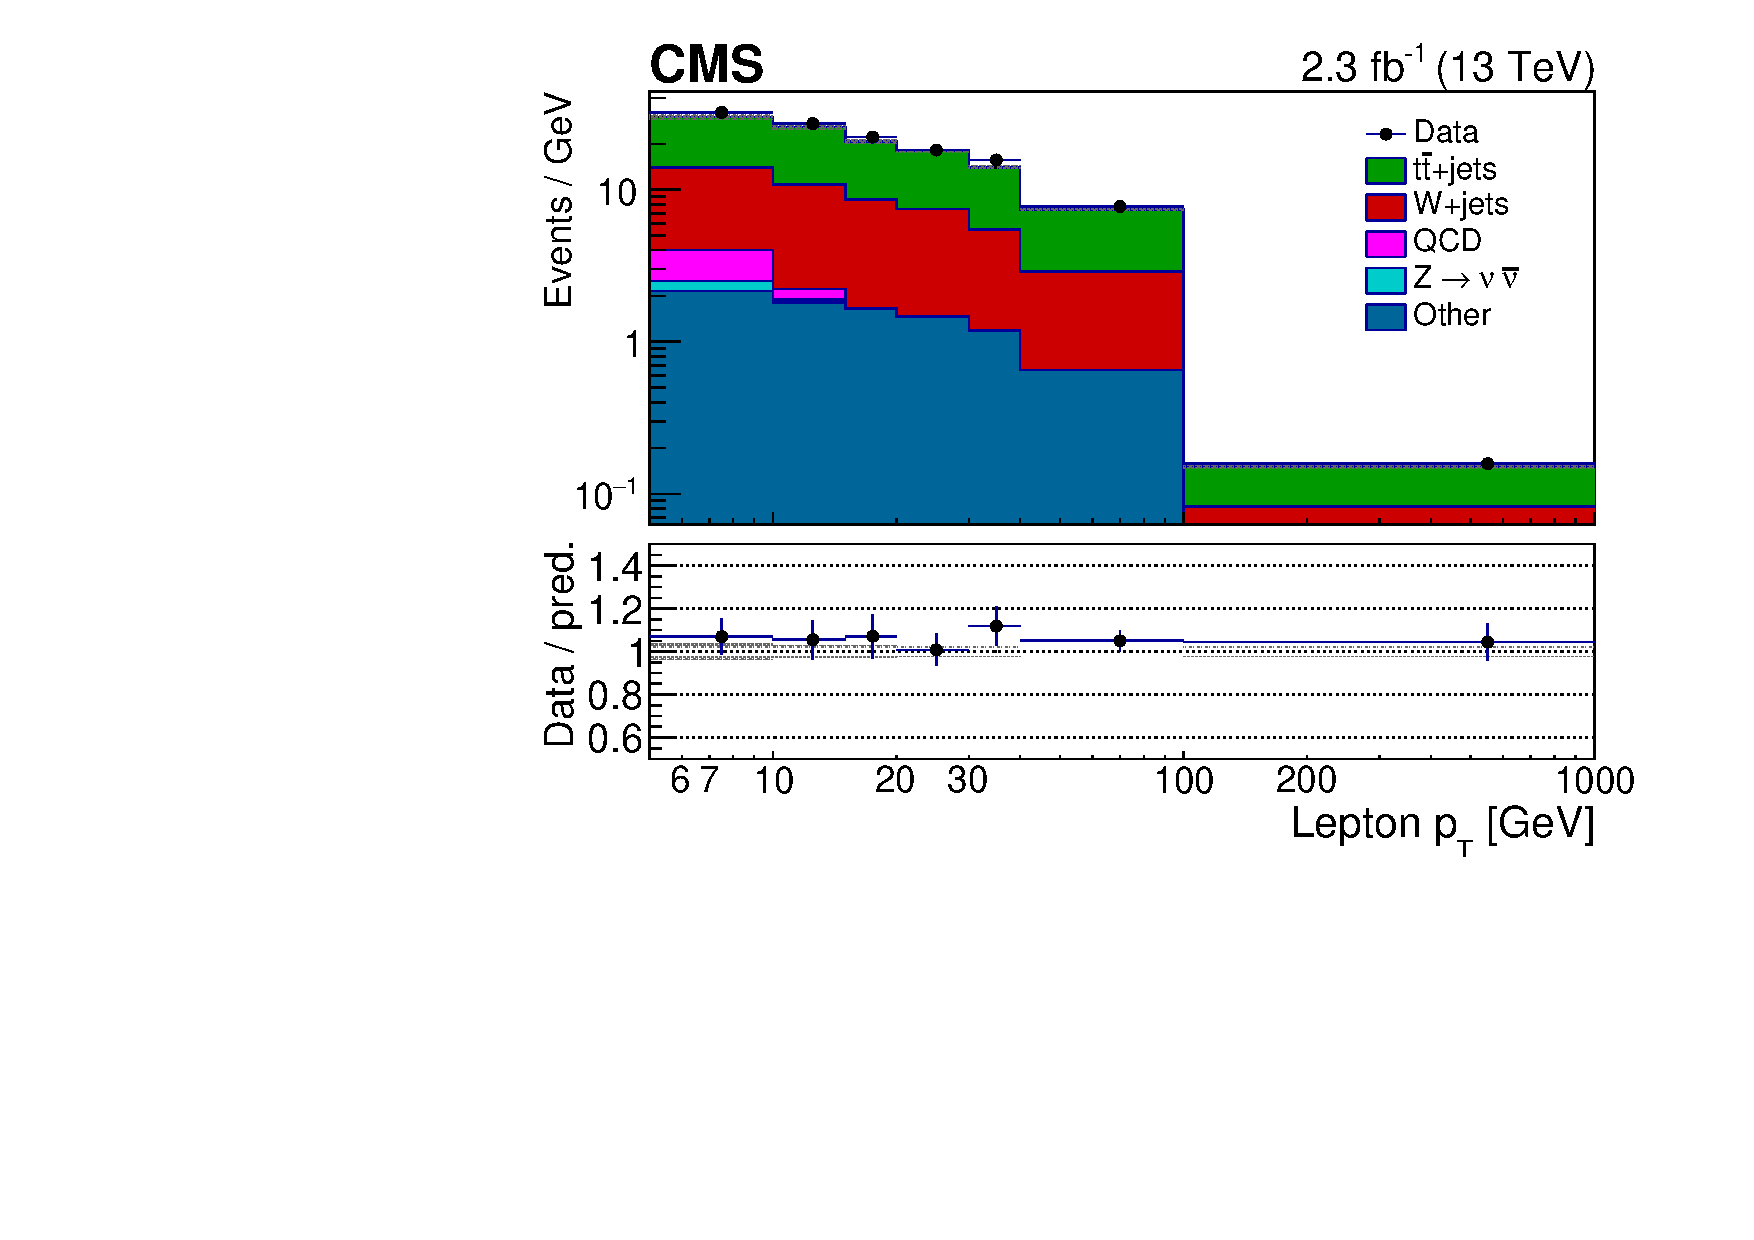
\includegraphics[width=0.49\textwidth]{figs/analysis13TeV/TTBarWJets/lep1Pt_VetoLeptonControlRegion_Density.pdf}}
\subfigure{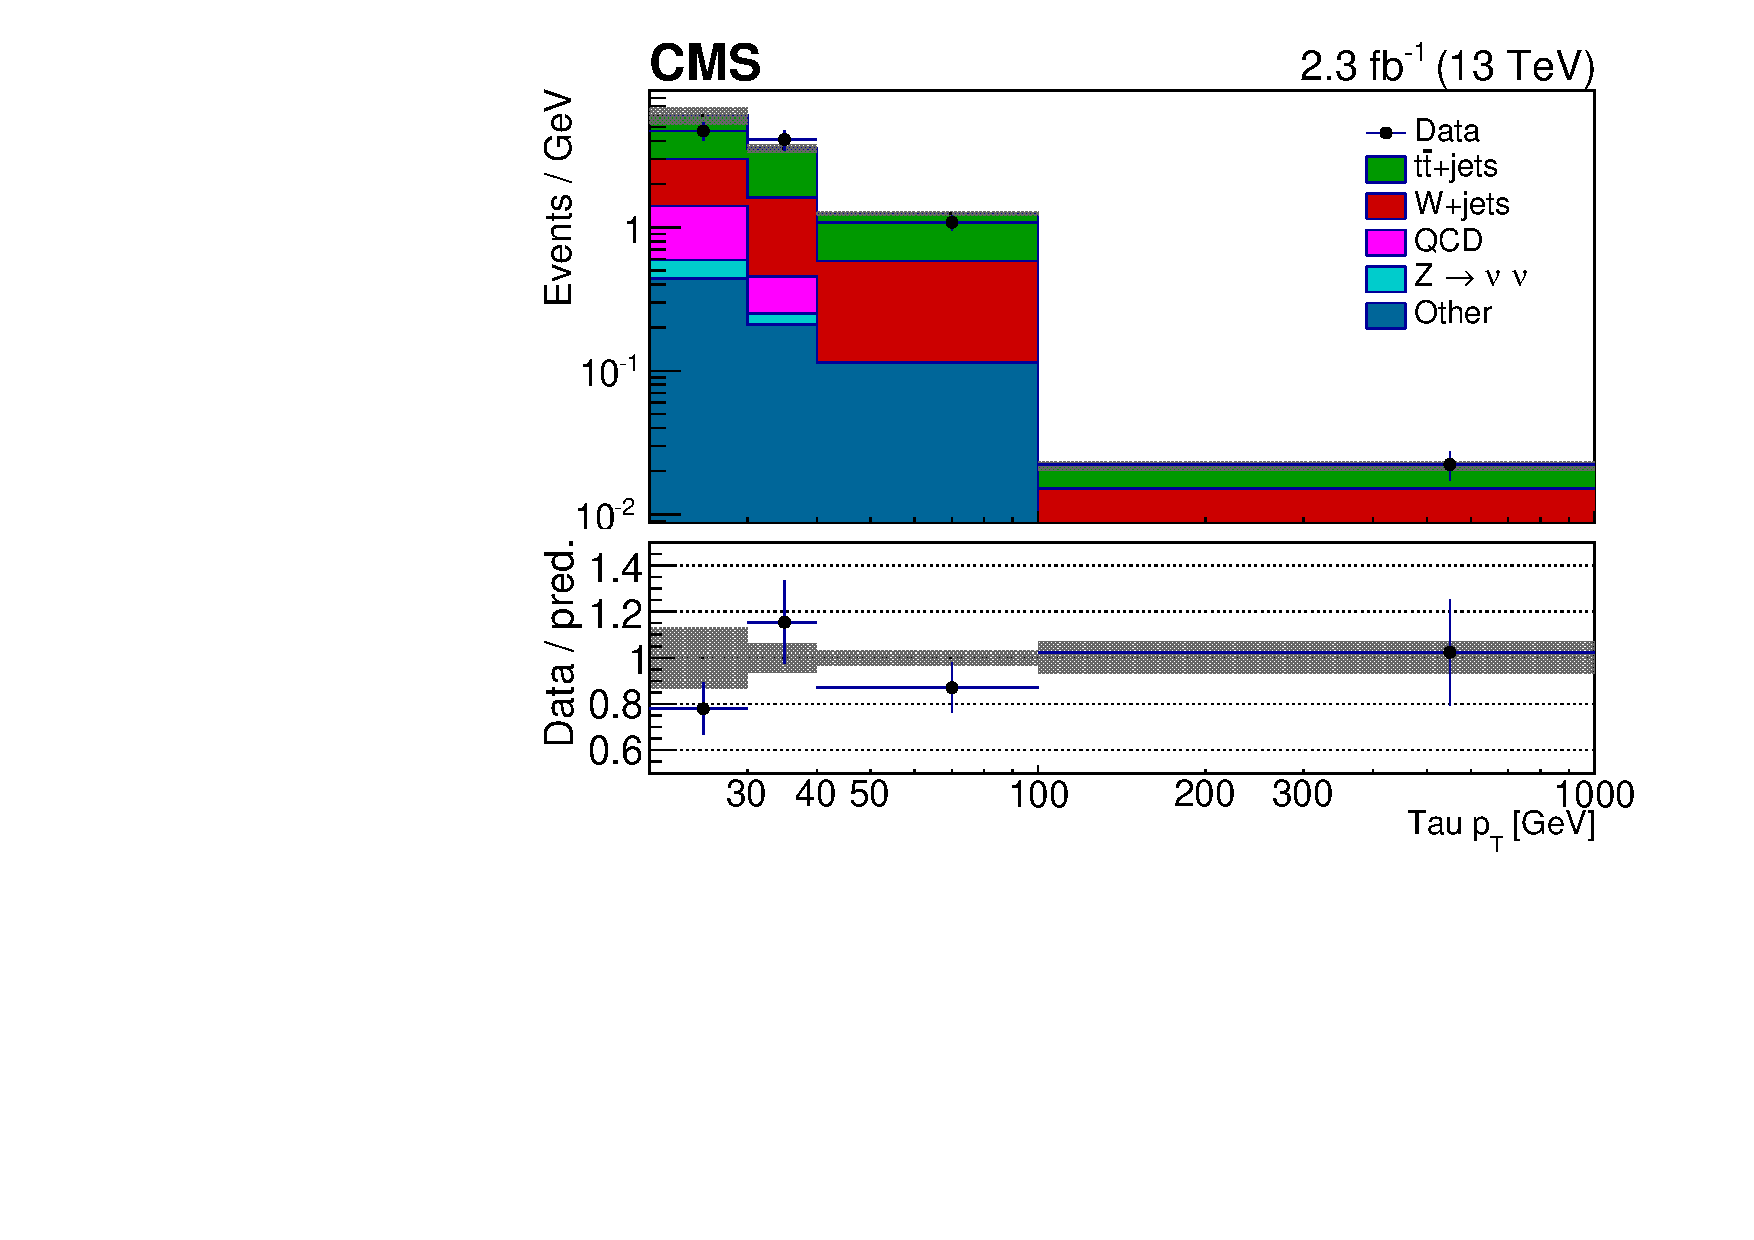
\includegraphics[width=0.49\textwidth]{figs/analysis13TeV/TTBarWJets/lep1Pt_VetoTauControlRegion_Density.pdf}}
\caption{ The $\pt$ distribution of the veto electron or muon (left) and the veto $\ensuremath{\tau_{\mathrm{h}}}$ (right)
is shown for events in the veto lepton control regions, comparing data with the MC prediction~\cite{CMS-PAS-SUS-15-004}. The $\ttbar$ and 
$\PW(\ell\nu)+$jets MC events have been reweighted according to the correction factors derived
in the $\ttbar$ enhanced and $\PW(\ell\nu)+$jets enhanced control regions, respectively.  
%The event yields in each bin are normalized by the bin width. 
The bottom panel shows the ratio of data to the background prediction, with uncertainties displayed as in Fig.~\ref{fig:TTBarWJetsCR_MR}.
}
\label{fig:VetoLeptonCR_LepPt}
\end{figure}

The $\ttbar$ background in the Electron and Muon Multijet categories is primarily from
the dilepton decay mode as the $M_{\mathrm{T}}$ requirement highly suppresses the semi-leptonic decay
mode. Corrections to the MC simulation derived from the $\ttbar$
control region primarily arise from semi-leptonic decays. 
We define an additional control region enhanced in dilepton $\ttbar$ decays 
to confirm that the MC corrections derived from a region dominated by
semi-leptonic decays also apply to dilepton decays. We select events with two tight leptons, 
both with $\pt>30 \GeV$, $\ETmiss>40\GeV$, and 
dilepton mass larger than $20\GeV$. For events with two leptons of the same flavor, we additionally
veto events with a dilepton mass between $76$ and $106\GeV$ in order to suppress background from $\cPZ$ boson
decays. At least one \PQb-tagged jet is required to enhance the purity for the $\ttbar$
process. Finally, we mimic the phase space region similar to our search region in the Electron and
Muon Multijet categories by treating one lepton as having failed the identification criteria 
and applying the $M_{\mathrm{T}}$ requirement using the other lepton. The correction factors measured in the 
$\ttbar$ control region are applied to the MC prediction of the dilepton
$\ttbar$ cross-check region in bins of $\MR$ and $\Rtwo$.
In Fig.~\ref{fig:WJets_TTBarDileptonCR_MRRsqUnrolled}
we show the ($\MR$,$\Rtwo$) distribution for the dilepton $\ttbar$ cross-check region
in events with four or more jets, and we observe no significant
mismodeling by the simulation, indicating that the measured corrections are accurate.

\clearpage

\subsubsection{The $\cPZ\to\nu\bar\nu$ background}
\label{sec:ZInvCR}

Three independent control regions are used to predict the $\cPZ(\nu\bar\nu)+$jets background,
relying on the assumption that the hadronic recoil spectrum and the jet multiplicity distribution
of the $\cPZ(\nu\bar\nu)+$jets process are similar to those of the $\PW(\ell\nu)+$jets and $\cPgg+$jets 
processes. The primary and most populated control region is the $\cPgg+$jets control region, 
defined by selecting events with at least one photon passing loose identification and
isolation requirements. The events are triggered using single-photon triggers, and 
the photon is required to have $\pt>50\GeV$. The momentum of the photon candidate
in the transverse plane is added vectorially to $\ptvecmiss$ 
in order to simulate an invisible particle, as one would have in the case of a 
$\cPZ\to\nu\bar\nu$ decay, and the $\MR$ and $\Rtwo$ variables are computed according to
this invisible decay scenario. 
% The requirements on $\MR$ and $\Rtwo$ sculpts the
% photon $\pt$ distribution, which turns on starting around $120\GeV$ and peaks at around
% $200\GeV$.  
A template fit to the distribution of $\sigma_{\eta\eta}$ is 
performed to determine the contribution from misidentified photons to the $\cPgg+$jets 
control region and is found to be about $5\%$, independent of the $\MR$ and $\Rtwo$. 
Events from the $\cPgg+$jets process where the photon is produced within the cone of a jet
(labeled as $\cPgg+$jets fragmentation) are considered to be background and subtracted
using the MC prediction. Backgrounds from rarer processes such as $\PW\cPgg$, $\cPZ\cPgg$, 
and $\ttbar\cPgg$ are also subtracted similarly.
In Fig.~\ref{fig:Znn_PhotonJets}, we show the $\MR$ distribution as well as the two-dimensional ($\MR$,$\Rtwo$) distribution for the $\cPgg+$jets control region, where we again 
observe a steeper $\MR$ falloff in the data compared to the simulation. Correction factors 
are derived in bins of $\MR$ and $\Rtwo$ and applied to the MC prediction for the 
$\cPZ\to\nu\bar\nu$ background in the search region. The statistical uncertainties for the 
correction factors range between $10\%$ and $30\%$ and are among the dominant uncertainties
for the $\cPZ\to\nu\bar\nu$ background prediction. 
Analogous to the procedure for the $\ttbar$ and $\PW(\ell\nu)+$jets control region, we derive an additional correction
factor of $0.87 \pm 0.05$ to accurately describe the yield in events with four or more jets. Additional
cross-checks are performed in bins of the number of b-tagged jets and systematic uncertainties ranging
from $4\%$ for events with zero b-tagged jets to $58\%$ for events with three or more b-tagged jets are
derived.

\begin{figure}[!ptb] \centering
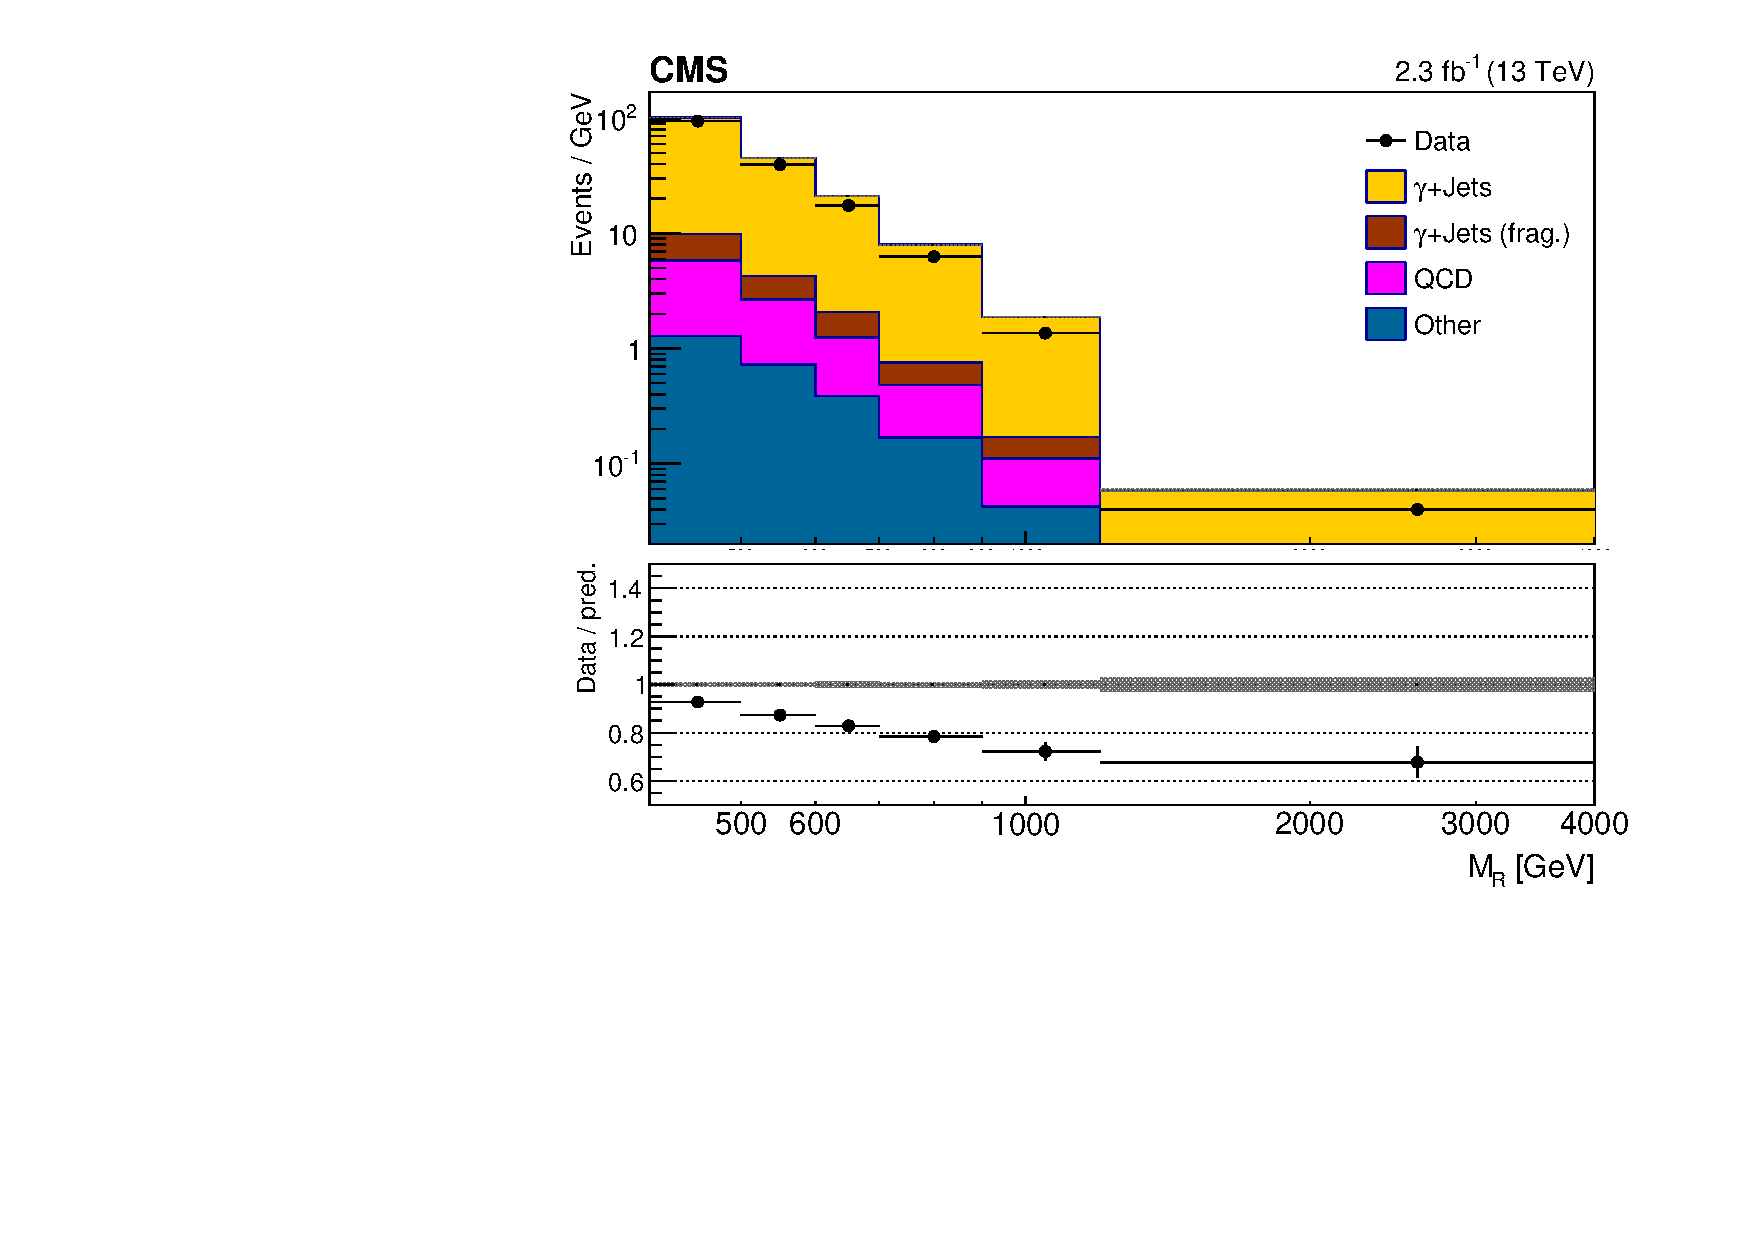
\includegraphics[width=0.9\textwidth]{figs/analysis13TeV/Znunu/Razor_PhotonControlRegion_MR_PhotonCR_Logy.pdf} \\
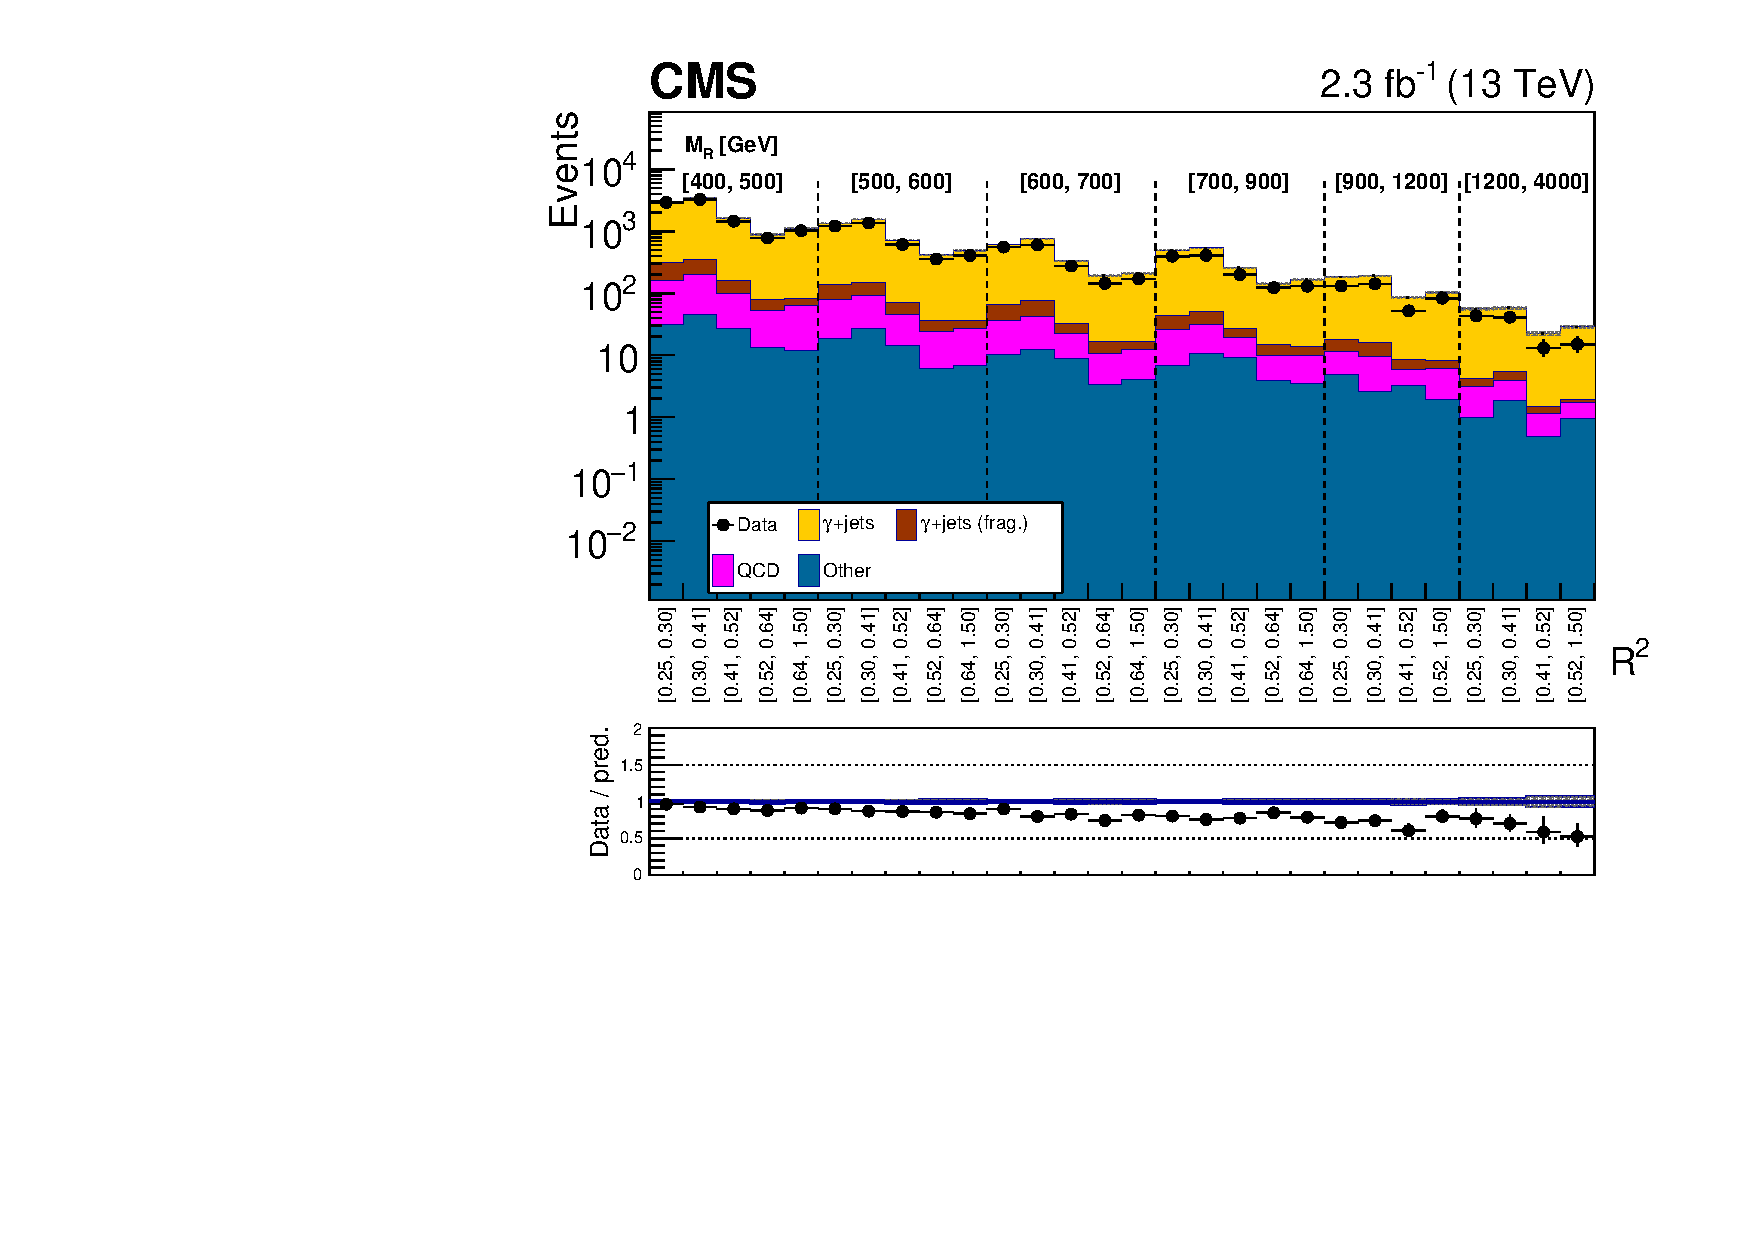
\includegraphics[width=0.9\textwidth]{figs/analysis13TeV/Znunu/Razor_PhotonControlRegion_MRRsqUnrolled_PhotonCR_Logy.pdf}
\caption{The one-dimensional distribution of $\MR$ in the $\cPgg$+jets control region
  (above) and the two-dimensional $\MR$-$\Rtwo$ distribution in
  the $\cPgg$+jets control region (below) are shown. The two-dimensional $\MR$-$\Rtwo$ distribution 
  is shown in a one-dimensional representation as in Fig.~\ref{fig:WJets_TTBarDileptonCR_MRRsqUnrolled}.
The bottom panel shows the ratio of data to the background prediction, with uncertainties displayed as in Fig.~\ref{fig:TTBarWJetsCR_MR}.
} 
\label{fig:Znn_PhotonJets}
\end{figure}


The second control region, enhanced in the $\PW(\ell\nu)+$jets, is defined
identically to the $\PW(\ell\nu)+$jets control region described in Section~\ref{sec:TTBarWJetsCR}, except that the lepton is treated as invisible
by adding its momentum vectorially to $\ptvecmiss$, and the $\MR$ and $\Rtwo$
variables are computed accordingly. Correction factors are computed using events from this control region,
and the difference between these correction factors and those computed from the $\cPgg+$jets control region
is propagated as a systematic uncertainty.  These uncertainties range between $10\%$ and $40\%$ depending on the ($\MR$,$\Rtwo$) bin. 

The third control region, enhanced in $\cPZ\to\ell^+\ell^-$ decays, 
is defined by selecting events with two tight electrons or two tight muons, and requiring that the dilepton mass is
between $76$ and $106\GeV$. Events are required to have no \PQb-tagged jets
in order to suppress $\ttbar$ background. The two leptons are treated as invisible by adding their
momenta vectorially to $\ptvecmiss$. We apply the correction factors obtained from the
$\cPgg+$jet control region to the $\cPZ\to\ell^+\ell^-$ MC prediction and perform a cross-check against data
in this control region. No significant discrepancy between the data and the prediction is observed.


\subsubsection{The QCD multijet background}
\label{sec:QCDCR}

The QCD multijet processes contribute about $10\%$ of the total background in the zero-lepton Multijet
event category for bins with zero or one \PQb-tagged jets. Such events enter the search regions
in the tails of the \MET distribution when the energy of 
one of the jets in the event is significantly under- or over-measured. 
In most such situations, the \ptvecmiss points either toward
or away from the leading jets and therefore the two megajets tend to
be in a back-to-back configuration. The search region is defined by requiring that
the azimuthal angle between the two megajets $\Delta\phi_R$ be less than
$2.8$, which was found to be an optimal selection based on studies
of QCD multijet and signal simulated samples. We define the control region for the QCD background process to be events
with $\dPhiR>2.8$, keeping all other selection requirements identical to those for
the search region. The purity of the QCD multijet process in the control region
is more than $70\%$. 

After subtracting the non-QCD background,
we project the observed data yield in the control region to the search region using
the translation factor $\zeta$:
\begin{equation}
\zeta = \frac{N(|\dPhiR|<2.8)}{N(|\dPhiR|>2.8)},
\end{equation}
where the numerator and denominator are the number of events
passing and failing the selection on $|\dPhiR|<2.8$, respectively. We
find that the translation factor calculated from the MC simulation
decreases as a function of $\MR$ and is, to a large degree, constant as a function of $\Rtwo$.
Using data events in the low $\Rtwo$ region ($0.15$ to $0.25$), dominated
by QCD multijet background, we measure the translation factor $\zeta$ as a function of
$\MR$ to cross-check the values obtained from the simulation.
The $\MR$ dependence of $\zeta$ is modeled as the sum of a power law
and a constant. This functional shape is fitted to the values of $\zeta$ calculated from the MC.
A systematic uncertainty of $87\%$ is propagated, covering both the
spread around the fitted model as a function of $\MR$ and $\Rtwo$ in
simulation, and the difference between the values measured in simulation
and data. The function used
for $\zeta$ and the values measured in data and simulation are
shown in Fig.~\ref{fig:QCDTranslationFactor}. 

\begin{figure}[!ptb]
\centering
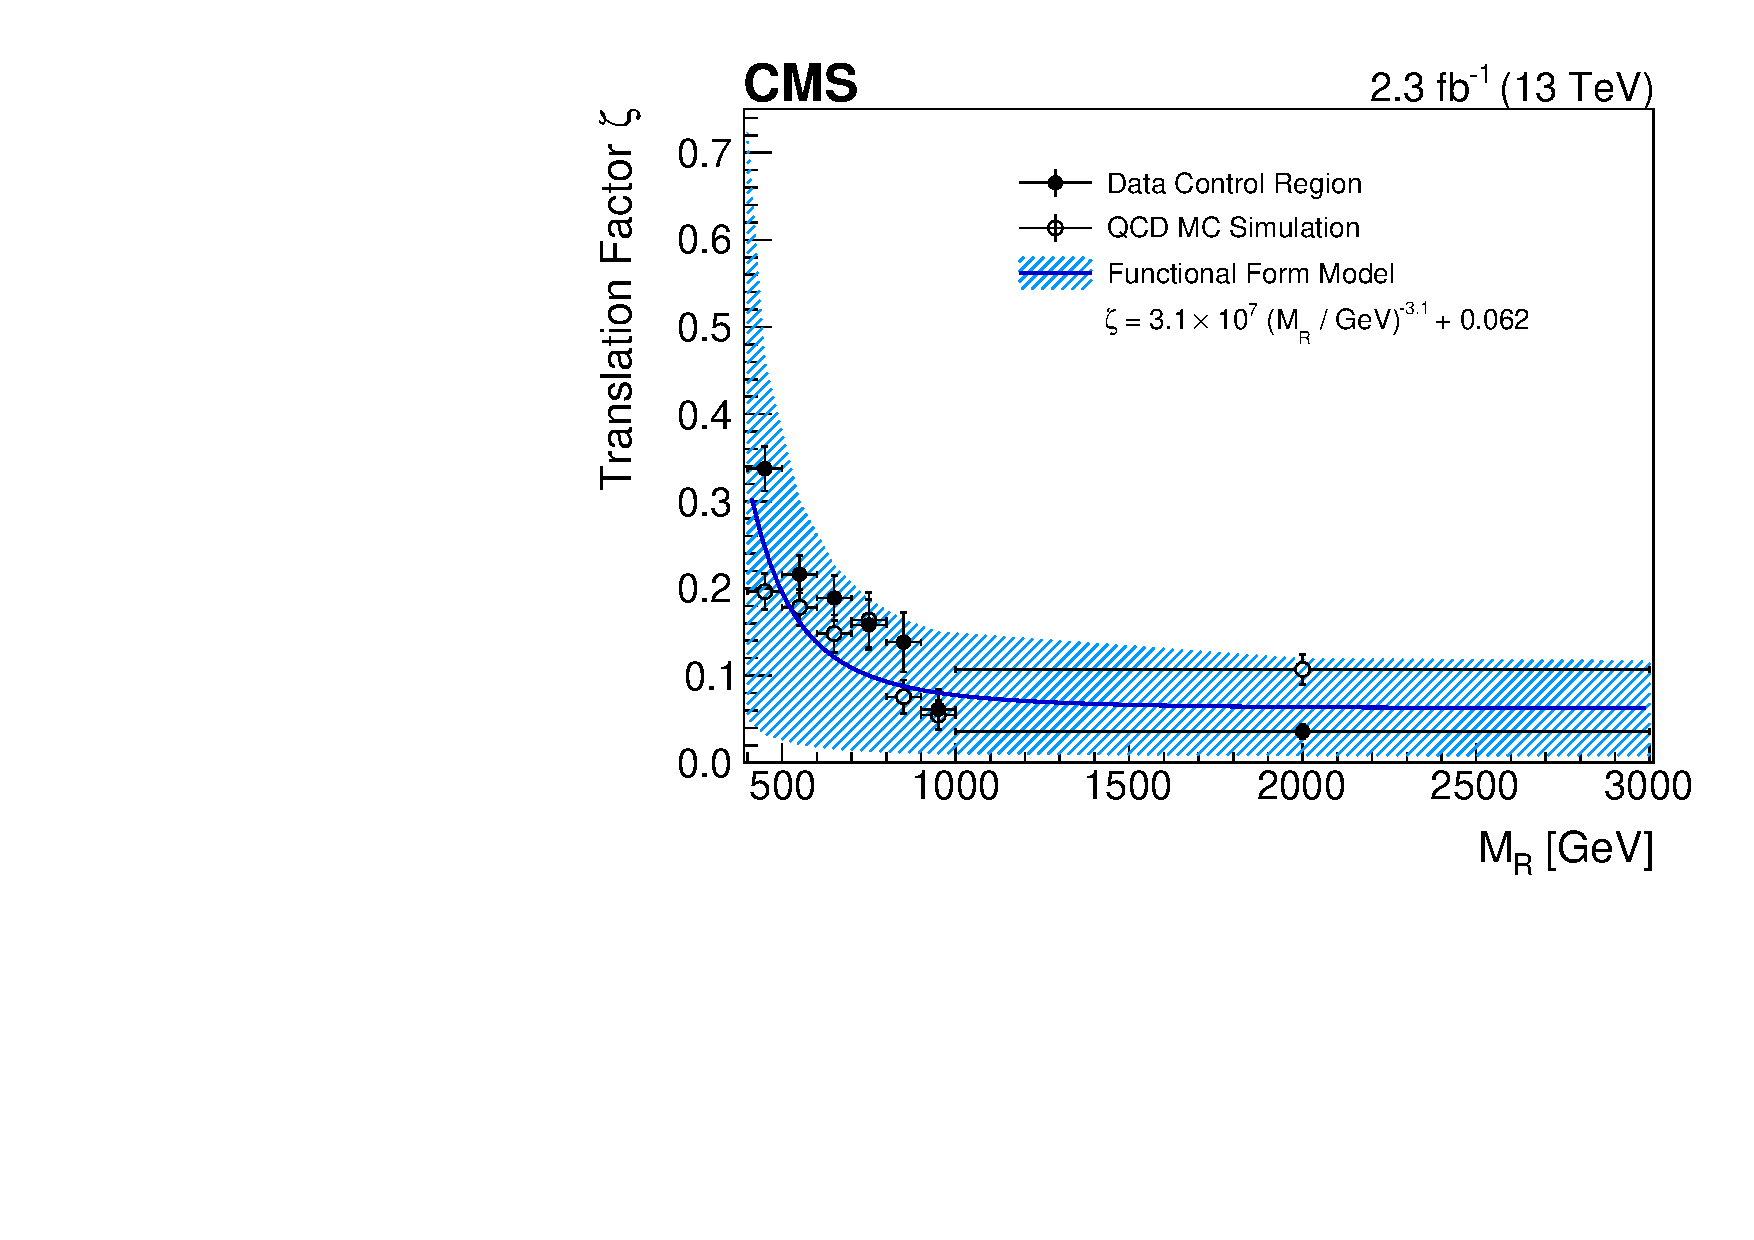
\includegraphics[width=0.75\textwidth]{figs/analysis13TeV/npf_vs_mr_razor_fit.pdf}
\caption{\label{fig:QCDTranslationFactor} 
The translation factor $\zeta$ is shown as a function of $\MR$~\cite{CMS-PAS-SUS-15-004}. The curve shows the 
functional form used to model the $\MR$ dependence, and the open circle
and black dot data points are  the values of $\zeta$ measured in the low-$\Rtwo$ data
control region and the QCD MC simulation, respectively. The hashed region indicates the size of the systematic uncertainty in
$\zeta$.}
\end{figure}

We perform two additional cross-checks on the accuracy of the MC prediction for
$\zeta$ in control regions dominated by processes similar to the QCD multijet
background with no invisible neutrinos in the final state. The first 
cross-check is performed on a dimuon control region enhanced in $\cPZ\rightarrow\Pgm^+\Pgm^-$ decays, 
and the second cross-check is performed on a dijet control region enhanced in QCD dijet events. 
In both cases, the events at large $\Rtwo$ result from cases similar to our search region
where the energy of a leading jet is severely mismeasured. We compare the values of
$\zeta$ measured in these data control regions to the values predicted
by the simulation and observe an agreement at the $20\%$ level, well within the 
systematic uncertainty of $87\%$ assigned to the QCD background estimate. 


\subsection{Method B: fit-based background prediction}
\label{sec:FitBkg}

The second background prediction method is based the same methodology
as the 8 \TeV search described in Sec.~\ref{sec:bmodel8TeV} along with
the modifications detailed above.

The sideband region is defined to be $100 \GeV$ in width in $\MR$
and $0.05$ in $\Rtwo$. Explicitly, for the
Multijet event category, it comprises the region $500 \GeV$
$< \MR < 600 \GeV$ and $\Rtwo > 0.3$, plus the region $\MR > 500 \GeV$
and $0.25 < \Rtwo < 0.3$.  For the Muon and Electron Multijet
event categories, it comprises the region $400 \GeV < \MR < 500 \GeV$
and $\Rtwo > 0.2$, plus the region $\MR > 400 \GeV$ and
$0.15 < \Rtwo < 0.2$. The updated sideband regions for the 13 \TeV
search are shown in Fig.~\ref{fig:regions13TeV}.

\begin{figure}[tpb!]
\centering
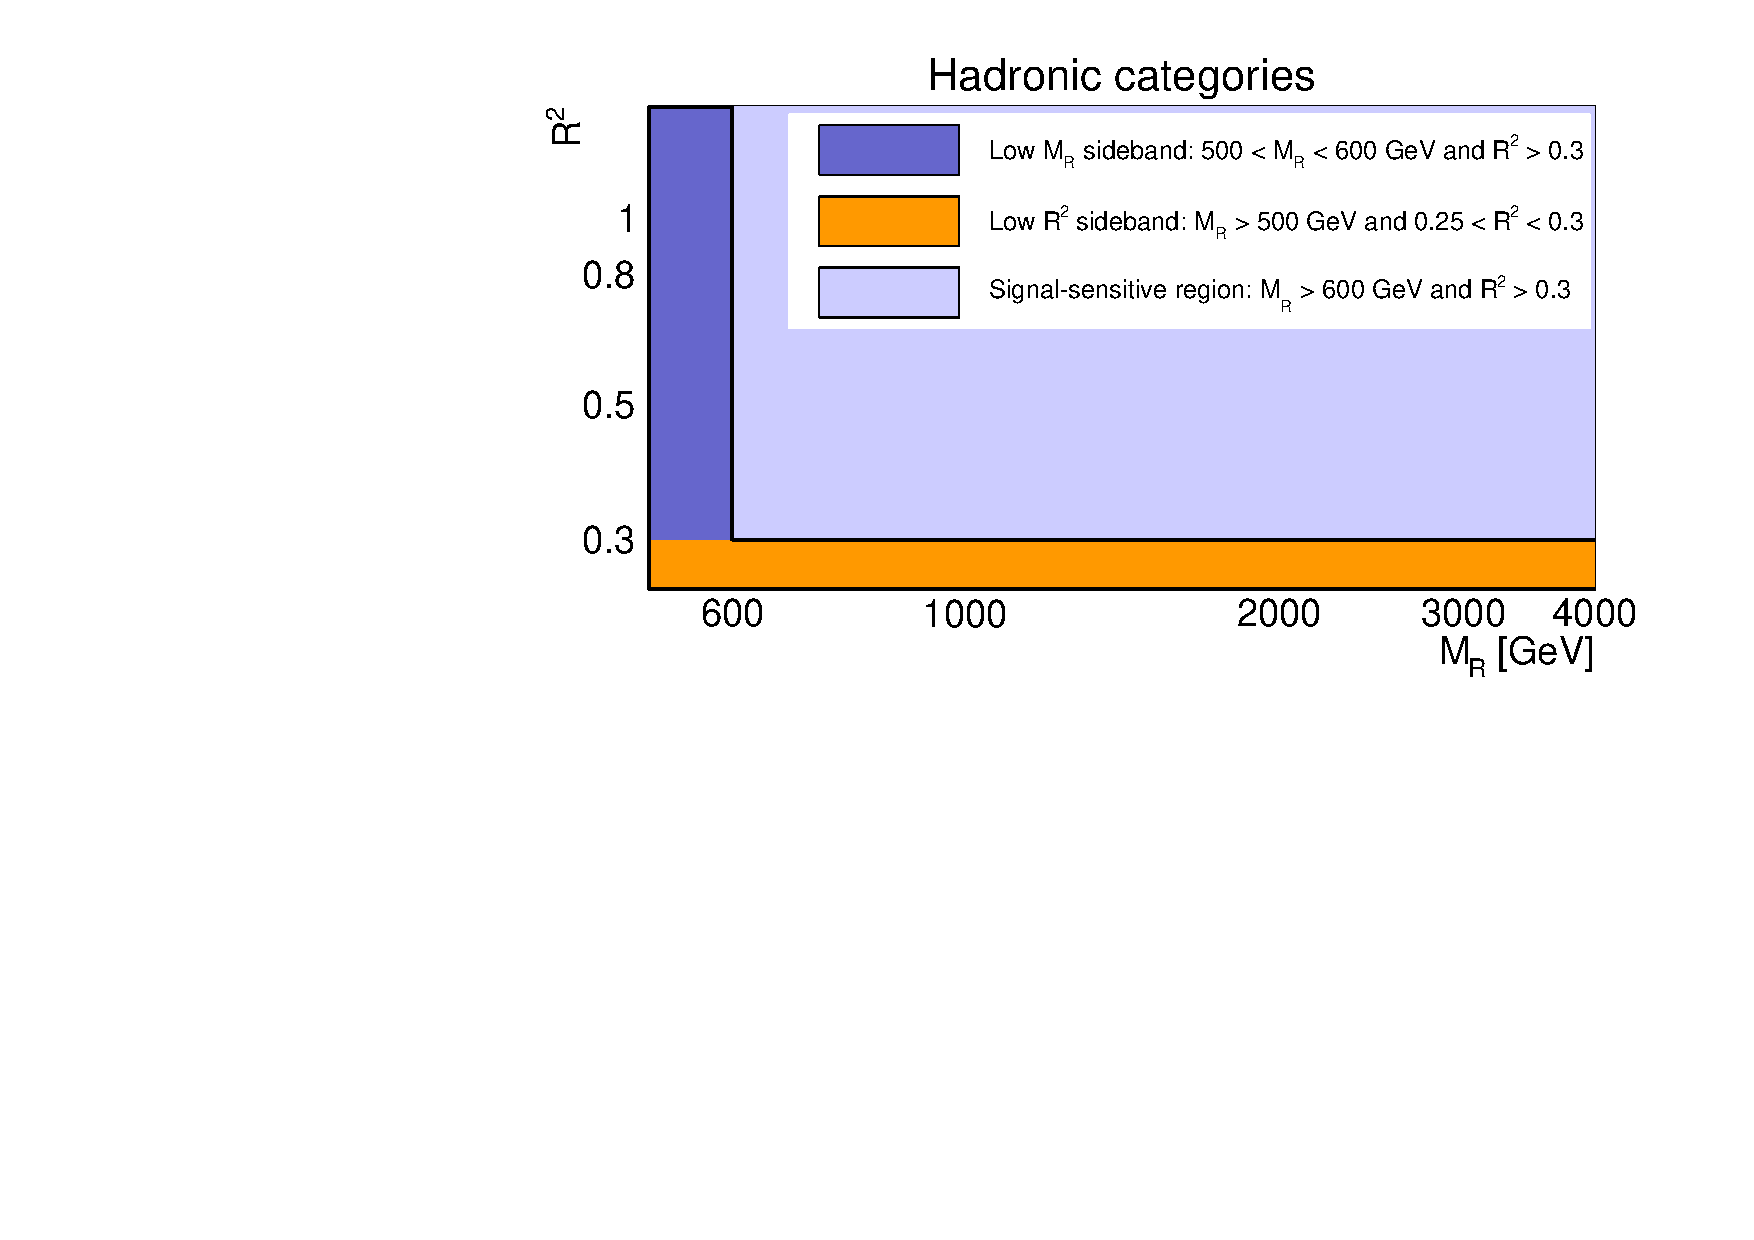
\includegraphics[width=0.9\textwidth]{figs/analysis13TeV/SidebandL_MultiJet.pdf}\\
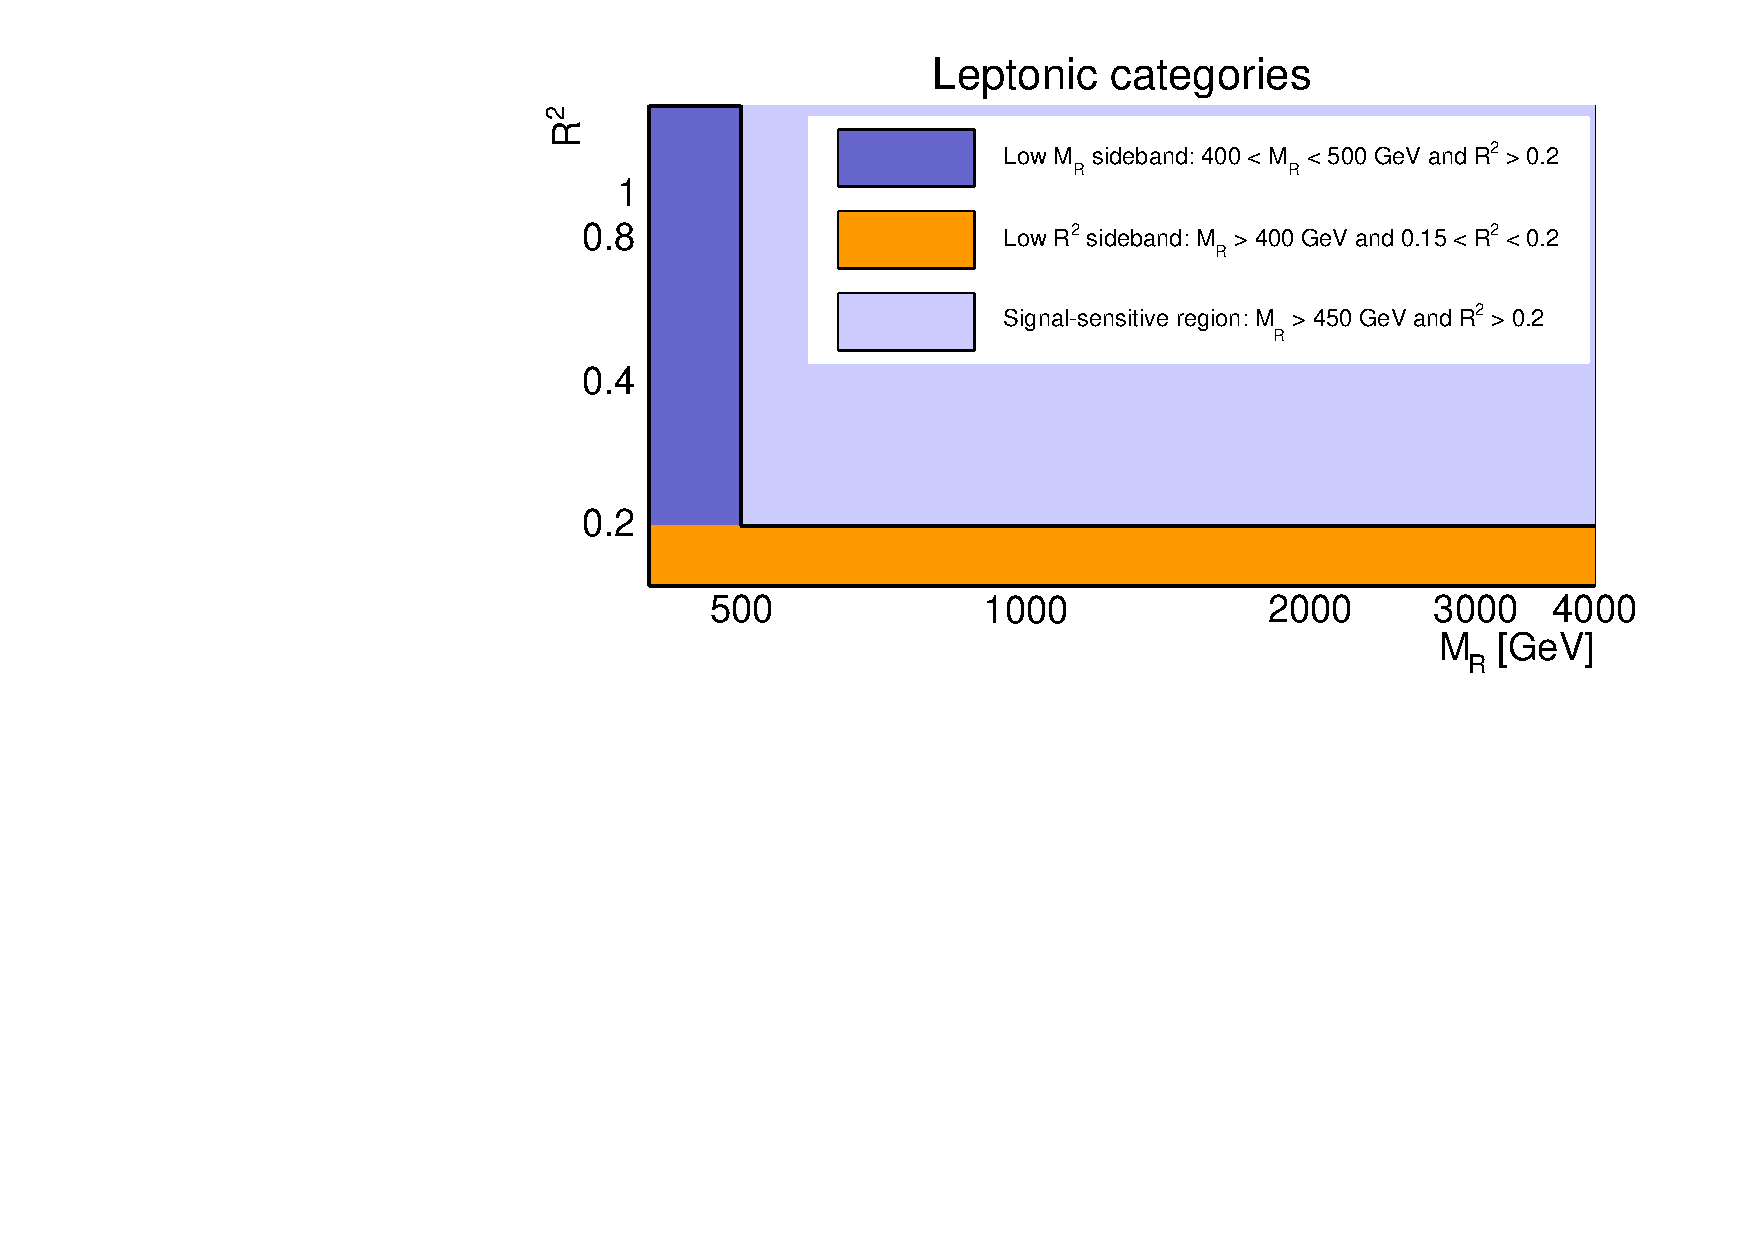
\includegraphics[width=0.9\textwidth]{figs/analysis13TeV/SidebandL_Mu.pdf}
\caption{\label{fig:regions13TeV} Updated definition of the sideband and the
 signal-sensitive regions used in the analysis, for (top) the Multijet
 category and (bottom) the other categories for the 13 \TeV search~\cite{jmgd}.}
\end{figure}

For each event category, we fit the two-dimensional distribution of 
$\MR$ and $\Rtwo$ in the sideband region using the
above functional form, separately for events with zero, one, two, and three or more \PQb-tagged jets. The
normalization in each event category and each \PQb-tagged jet bin is
independently varied in the fit. Due to the lack of data events in the category
with three or more \PQb-tagged jets, we constrain
the shape in this category to be related to the shape for events with two
\PQb-tagged jets as follows:
\begin{equation}
  f^{\geq 3\cPqb}_{\mathrm{SM}}(\MR, \Rtwo)  = (1+m_{\MR}(\MR - M^{\mathrm{offset}}_R))f^{2\cPqb}_{\mathrm{SM}}(\MR, \Rtwo),
\label{eq:3btagFunction}
\end{equation}
where $f^{2\cPqb}_{\mathrm{SM}}(\MR, \Rtwo)$ and $f^{\geq 3\cPqb}_{\mathrm{SM}}(\MR, \Rtwo)$ are the
probability density functions for events with two and with three or more \PQb-tagged jets,
respectively; $\MR^{\mathrm{offset}}$ is the lowest $\MR$ value in a particular
event category; and $m_{\MR}$ is an additional nuisance parameter constrained by a Gaussian distribution
centered at the value measured using the simulation and with a
100\% uncertainty. The above form for the shape of the background events 
with three or more \PQb-tagged jets is verified in simulation.

Numerous tests are performed to establish the robustness of the fit
model in adequately describing the underlying distributions. To
demonstrate that the background model gives an accurate description of the 
background distributions, we construct a representative
data set using MC samples, and perform the background fit using
the form given by Eqn.~(\ref{eq:razFun}). Goodness of fit is
evaluated by comparing the background prediction from the fit with the
prediction from the simulation. This procedure is performed
separately for each of the search categories and we find
that the fit function yields an accurate representation of the
background predicted by the simulation.

We also observe that the fit model is insensitive to variations of the background
composition predicted by the simulation in each event category by altering
relative contributions of the dominant backgrounds, performing a
new fit with the alternative background composition, and comparing
the new fit results to the nominal fit result. The contributions
of the main $\ttbar$, $\PW(\ell\nu)+$jets, and $\cPZ(\nu\bar\nu)$ backgrounds 
are varied by 30\%, and the rare backgrounds from QCD multijet and
$\mathrm{\ttbar}\cPZ$  processes are varied by 100\%. For the Muon and Electron Multijet event categories,
we also vary the contributions from the dileptonic and semi-leptonic decays
of the $\ttbar$ background separately by 30\%. In each of these tests, we 
observe that the chosen functional form can adequately describe the shapes of 
the $\MR$ and $\Rtwo$ distributions as predicted by the modified MC simulation.

Additional pseudoexperiment studies are performed comparing the background prediction
from the sideband fit and the full region fit to evaluate the average
deviation between the two fit predictions. We observe that 
the sideband fit and the full region fit predictions in the
signal-sensitive region differ by up to 15\% and we propagate an
additional systematic uncertainty to the sideband fit background
prediction to cover this average difference.

%The best fit background
%shape is used as a probability density function and sampled to
%obtain an ensemble of toy experiments. For each toy experiment,
%we perform a sideband fit and a full region fit, and the fit predictions
%for the background yield in the region at high $M_{R}$ and high $R^{2}$ 
%are compared on a toy-by-toy basis. For the zero lepton category,
%the region is defined as $M_{R}>700 \GeV$ and $R^{2}>0.41$, while
%for the one lepton categories, the region is defined as 
% $M_{R}>500 \GeV$ and $R^{2}>0.25$. 
%Based on an ensemble of peusdo-experiments in which we sample a
%background-only pseudo-data set and then perform both a sideband fit
%and a full region fit, we observe that on average the sideband fit
%predicts a slightly smaller background yield in the signal-sensitive
%region compared to the full region fit and that the average relative
%difference decreases with increasing integrated luminosity.
%For the Multijet category, the average difference decreases
%from about 15\% for data samples corresponding to $2 \fbinv$
%to less than 2\% for data samples corresponding to about $20 \fbinv$,
%while for the one-lepton categories, the average difference
%decreases from about 15\% to about 7\%. The average difference is small 
%compared to the total systematic uncertainty, which ranges from 40\%
%to 100\% depending on the \PQb-tag bin. Nonetheless, we propagate an
%additional systematic uncertainty to the sideband fit background
%prediction to cover these average differences.

\begin{figure}[!ptb] \centering
\subfigure{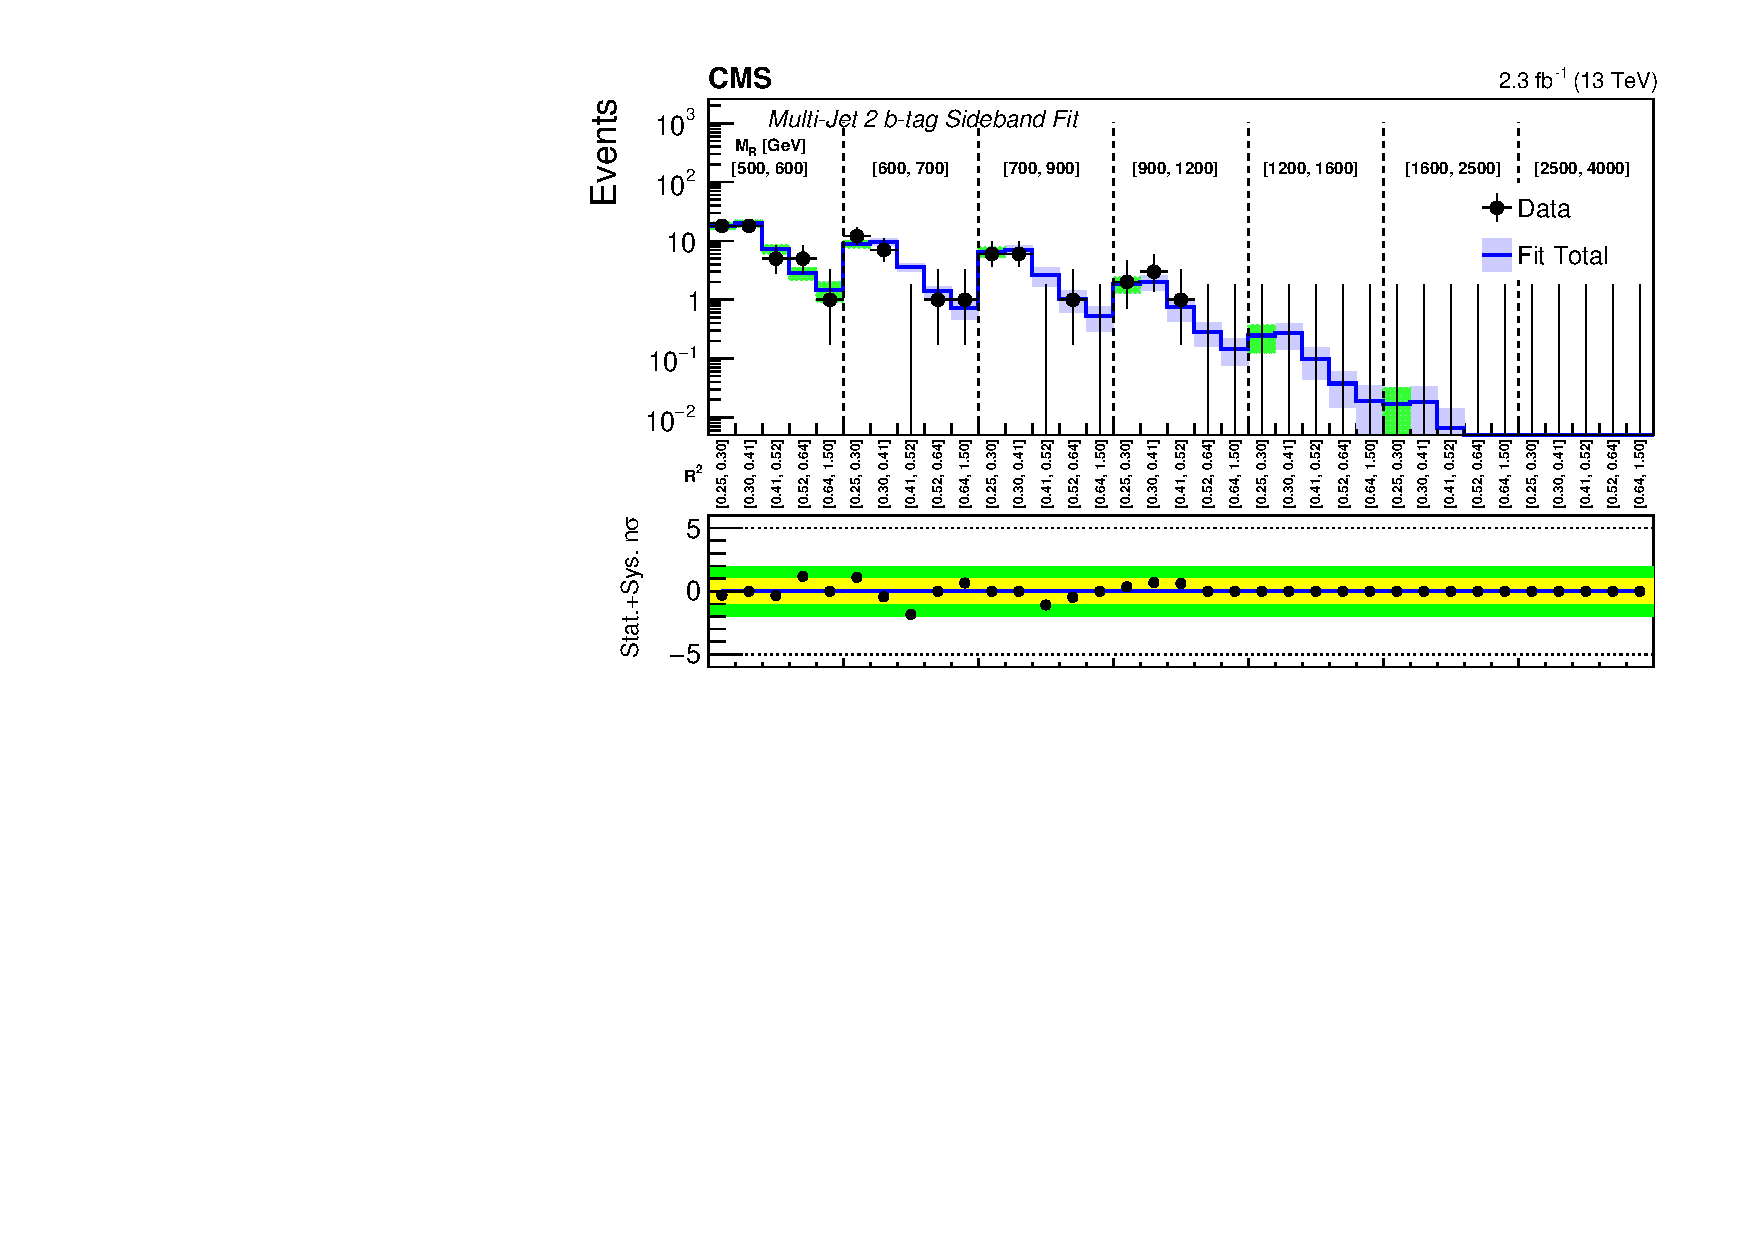
\includegraphics[width=0.9\textwidth]{figs/analysis13TeV/results/h_th1x_ns_2btag_MultiJet.pdf}}\\
\subfigure{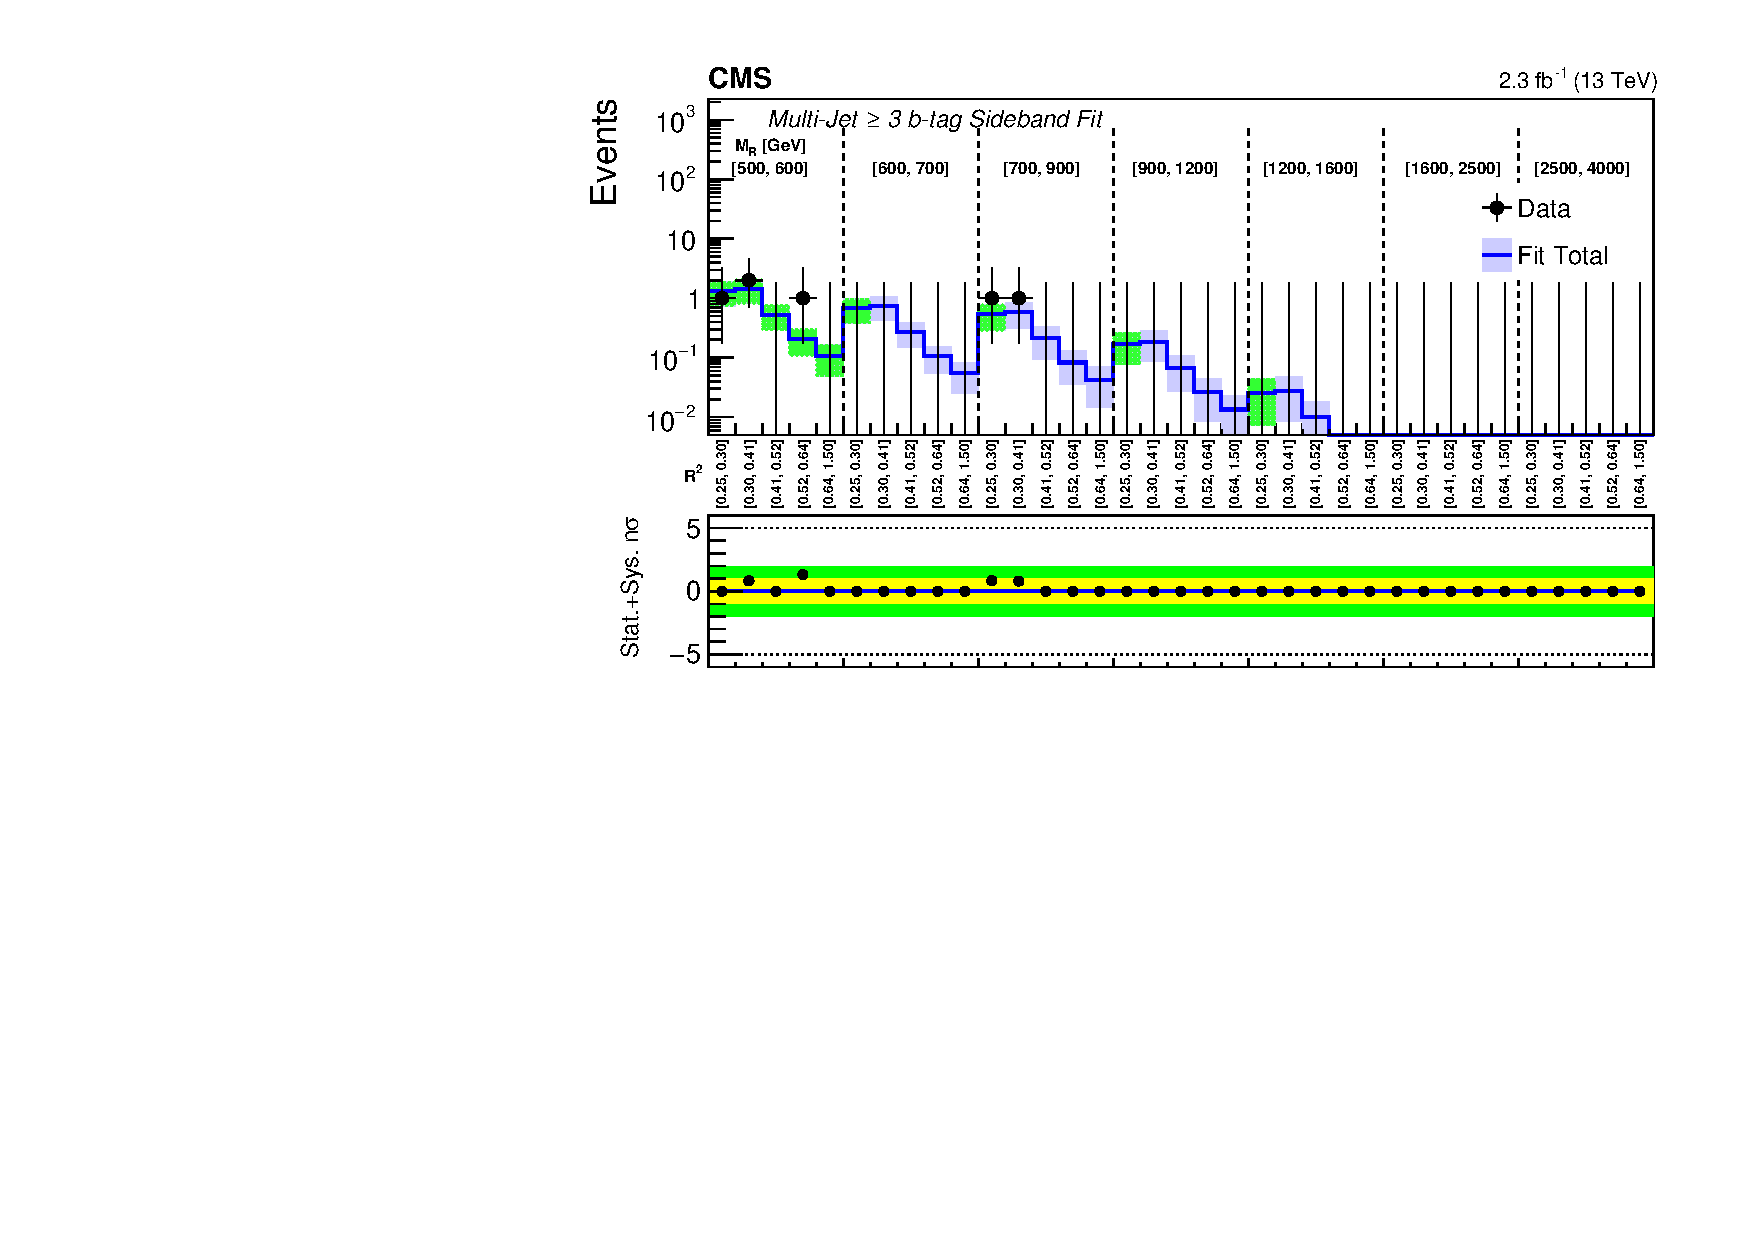
\includegraphics[width=0.9\textwidth]{figs/analysis13TeV/results/h_th1x_ns_3btag_MultiJet.pdf}}
\caption{Comparison of the sideband fit background prediction with the observed data
  in bins of $\MR$ and $\Rtwo$ variables in the Multijet category for
  the 2 \PQb-tag (upper) and $\geq 3$ \PQb-tag (lower) bins~\cite{CMS-PAS-SUS-15-004,jmgd}. Vertical dashed lines denote the 
  boundaries of different $\MR$ bins. On the
  upper panels, the colored bands represent the 
  systematic uncertainties in the background prediction, and the uncertainty bands for the 
  sideband bins are shown in green. On the bottom panels, the deviations between the observed 
  data and the background prediction are plotted in units of standard
  deviation ($\sigma$), taking into 
  account both statistical and systematic uncertainties. The green
  and yellow horizontal bands show the boundaries of 1 and 2 $\sigma$. }
\label{fig:results_Multijet2btag3btag}
\end{figure}
\begin{figure}[!ptb] \centering
\subfigure{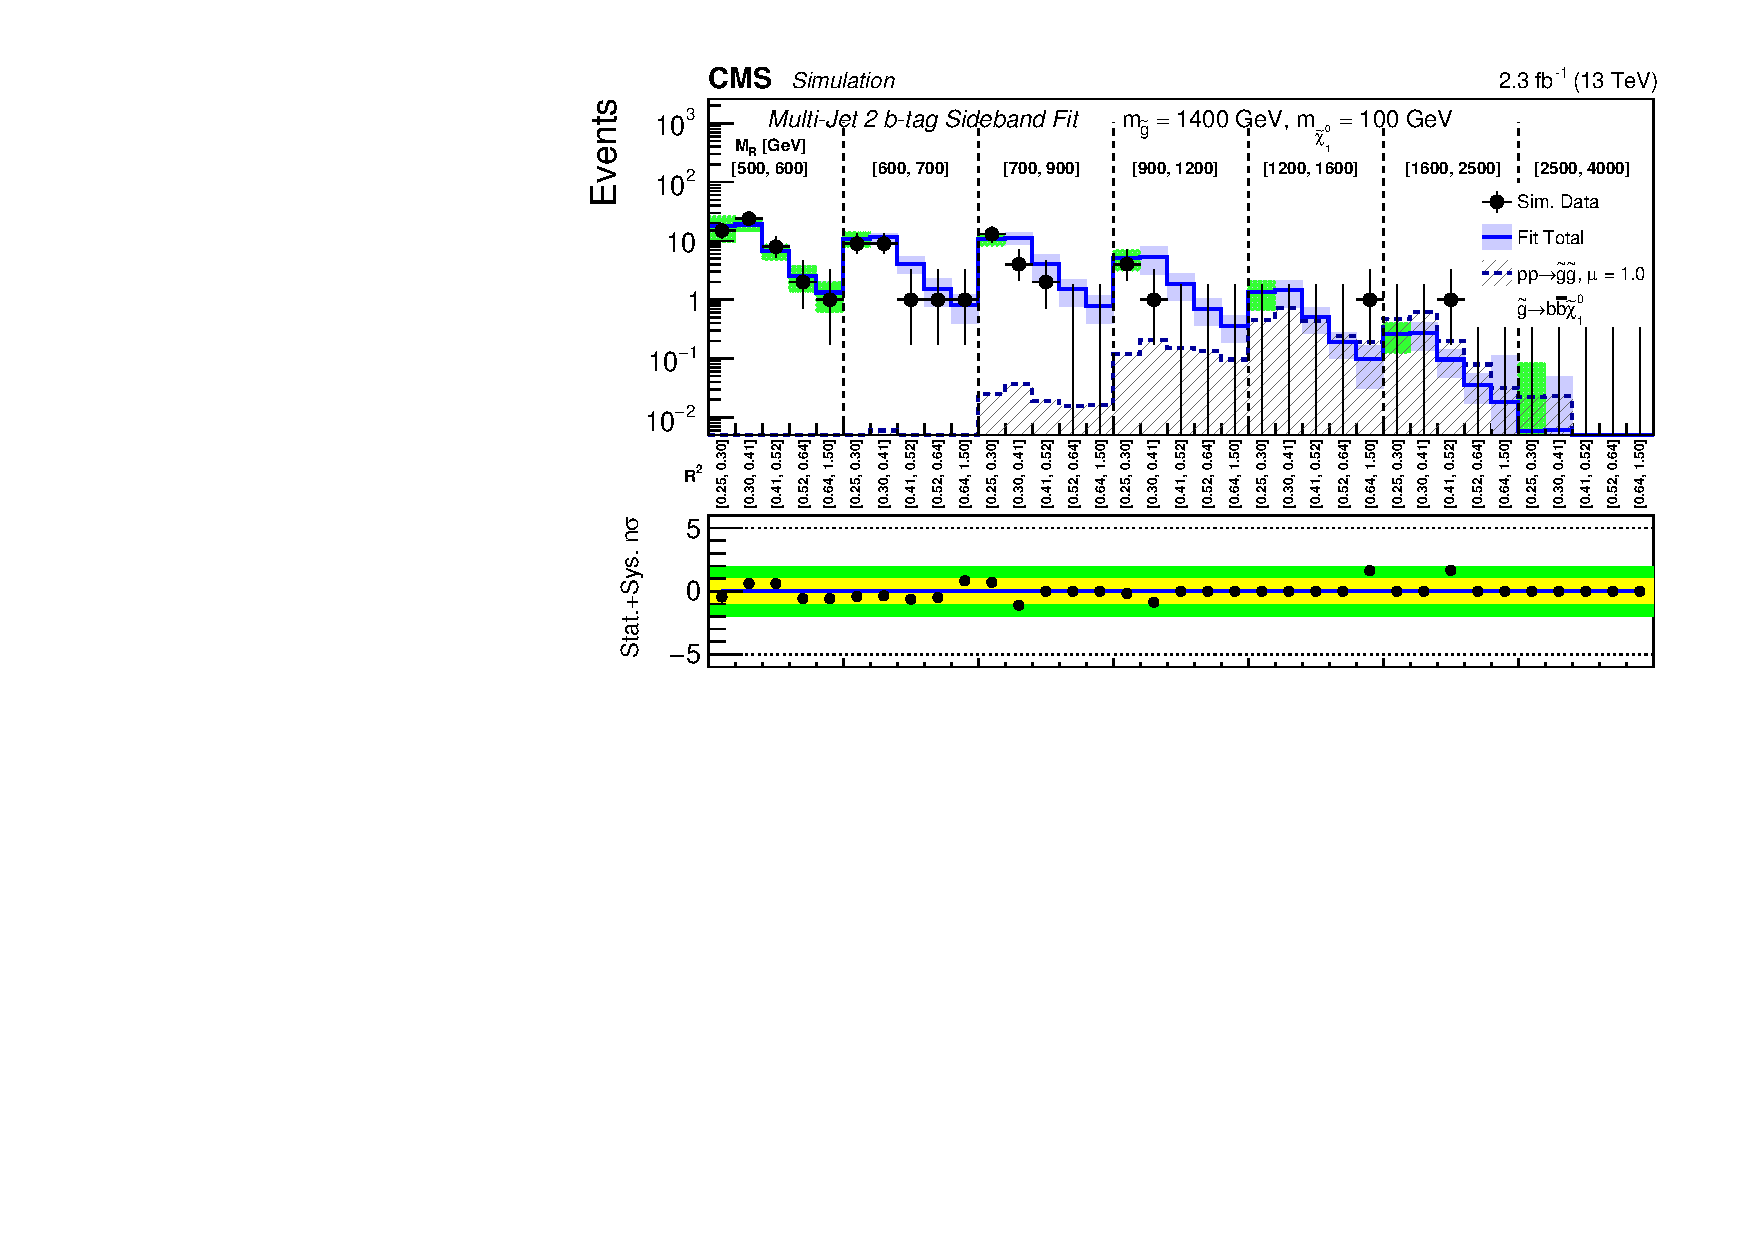
\includegraphics[width=0.9\textwidth]{figs/analysis13TeV/signalInjectionTests/T1bbbb_1400_100/h_th1x_ns_2btag_MultiJet.pdf}}\\
\subfigure{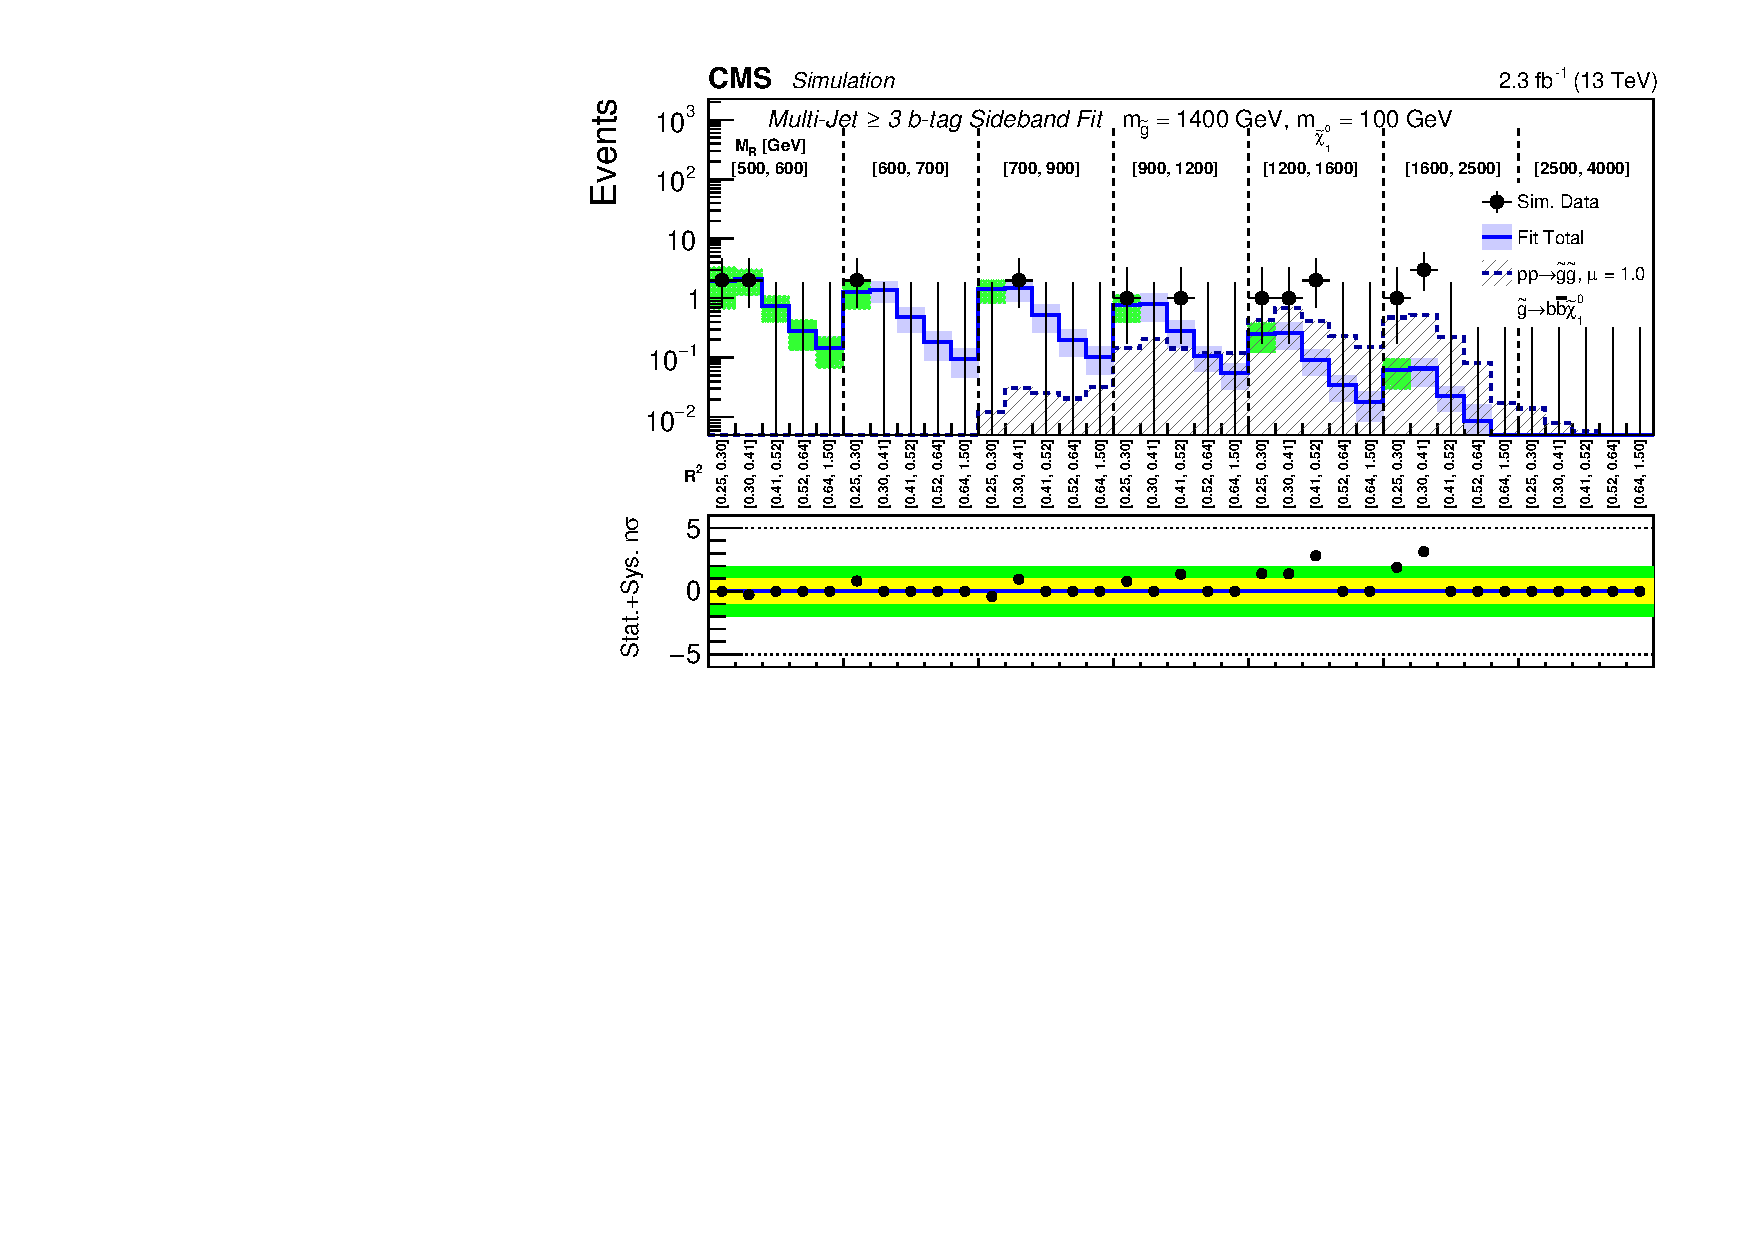
\includegraphics[width=0.9\textwidth]{figs/analysis13TeV/signalInjectionTests/T1bbbb_1400_100/h_th1x_ns_3btag_MultiJet.pdf}}
\caption{The result of the background-only fit performed in the
  sideband of the 2 \PQb-tag (upper) and $\geq 3$ \PQb-tag (lower) bins of the
  Multijet category on a signal-plus-background pseudodata set assuming a gluino pair production simplified
model signal, where gluinos decay with a 100\% branching fraction to a $\bbbar$ pair and the
 LSP, with $m_{\sGlu} = 1.4 \TeV$ and  $m_{\chiz_1}=100 \GeV$, at
 nominal signal strength~\cite{CMS-PAS-SUS-15-004,jmgd}. A detailed explanation of the figure format is given in the caption of
  Fig.~\ref{fig:results_Multijet2btag3btag}.}
\label{fig:signal_Multijet2btag3btag}
\end{figure}

To illustrate method B, we present the data and fit-based background predictions 
in Fig.~\ref{fig:results_Multijet2btag3btag}, for events in the 2 \PQb-tag and $\geq 3$ \PQb-tag 
Multijet categories. The number of events observed in data is compared to the
prediction from the sideband fit in the $\MR$ and $\Rtwo$ bins. To
quantify the agreement between the background model and the observation, we generate 
alternative sets of background shape parameters from the covariance matrix calculated
by the fit. An ensemble of pseudoexperiment data sets is created, generating 
random ($\MR$, $\Rtwo$) pairs distributed according to each of these alternative shapes. 
For each ($\MR$,$\Rtwo$) bin, the distribution of the predicted yields from the
ensemble of pseudoexperiments is compared to the observed yield in data. 
The agreement between the predicted and the observed yields is described as a two-sided 
p-value and translated into the corresponding number of standard deviations for a normal
distribution. Positive (negative) significance indicates the observed
yield is larger (smaller) than the predicted one. We find that the pattern of 
differences between data and background predictions in the different
bins considered is consistent with statistical fluctuations.

To demonstrate that the model-independent sideband fit procedure
used in the analysis would be sensitive to the presence of a
signal, we perform a signal injection test. We sample a signal-plus-background 
pseudo-data set and perform a background-only fit in the sideband. We show one illustrative 
example of such a test in Fig.~\ref{fig:signal_Multijet2btag3btag}, where we inject a signal 
corresponding to gluino pair production, in which each gluino decays to a neutralino and 
a $\bbbar$ pair with $m_{\sGlu} = 1.4 \TeV$ and $m_{\chiz_1}=100 \GeV$. The
deviations with respect to the fit predictions are shown for the 2
\PQb-tag and $\geq 3$ \PQb-tag Multijet categories. We observe characteristic patterns 
of excesses in two adjacent groups of bins neighboring in $\MR$. 

For completeness, in Figs.~\ref{fig:results_Multijet0btag1btag}-\ref{fig:results_EleMultijet2btag3btag},
we present the results of the search for SUSY signal
events in the remaining categories, namely the 0 \PQb-tag and 1
\PQb-tag bins of the Multijet category, the four \PQb-tag bins of the Muon
Multijet category, and
the four \PQb-tag bins of the Electron Multijet
category. No statistically significant deviations from the expected
background predictions are observed in these categories in data.

\begin{figure}[!ptb] \centering
\subfigure{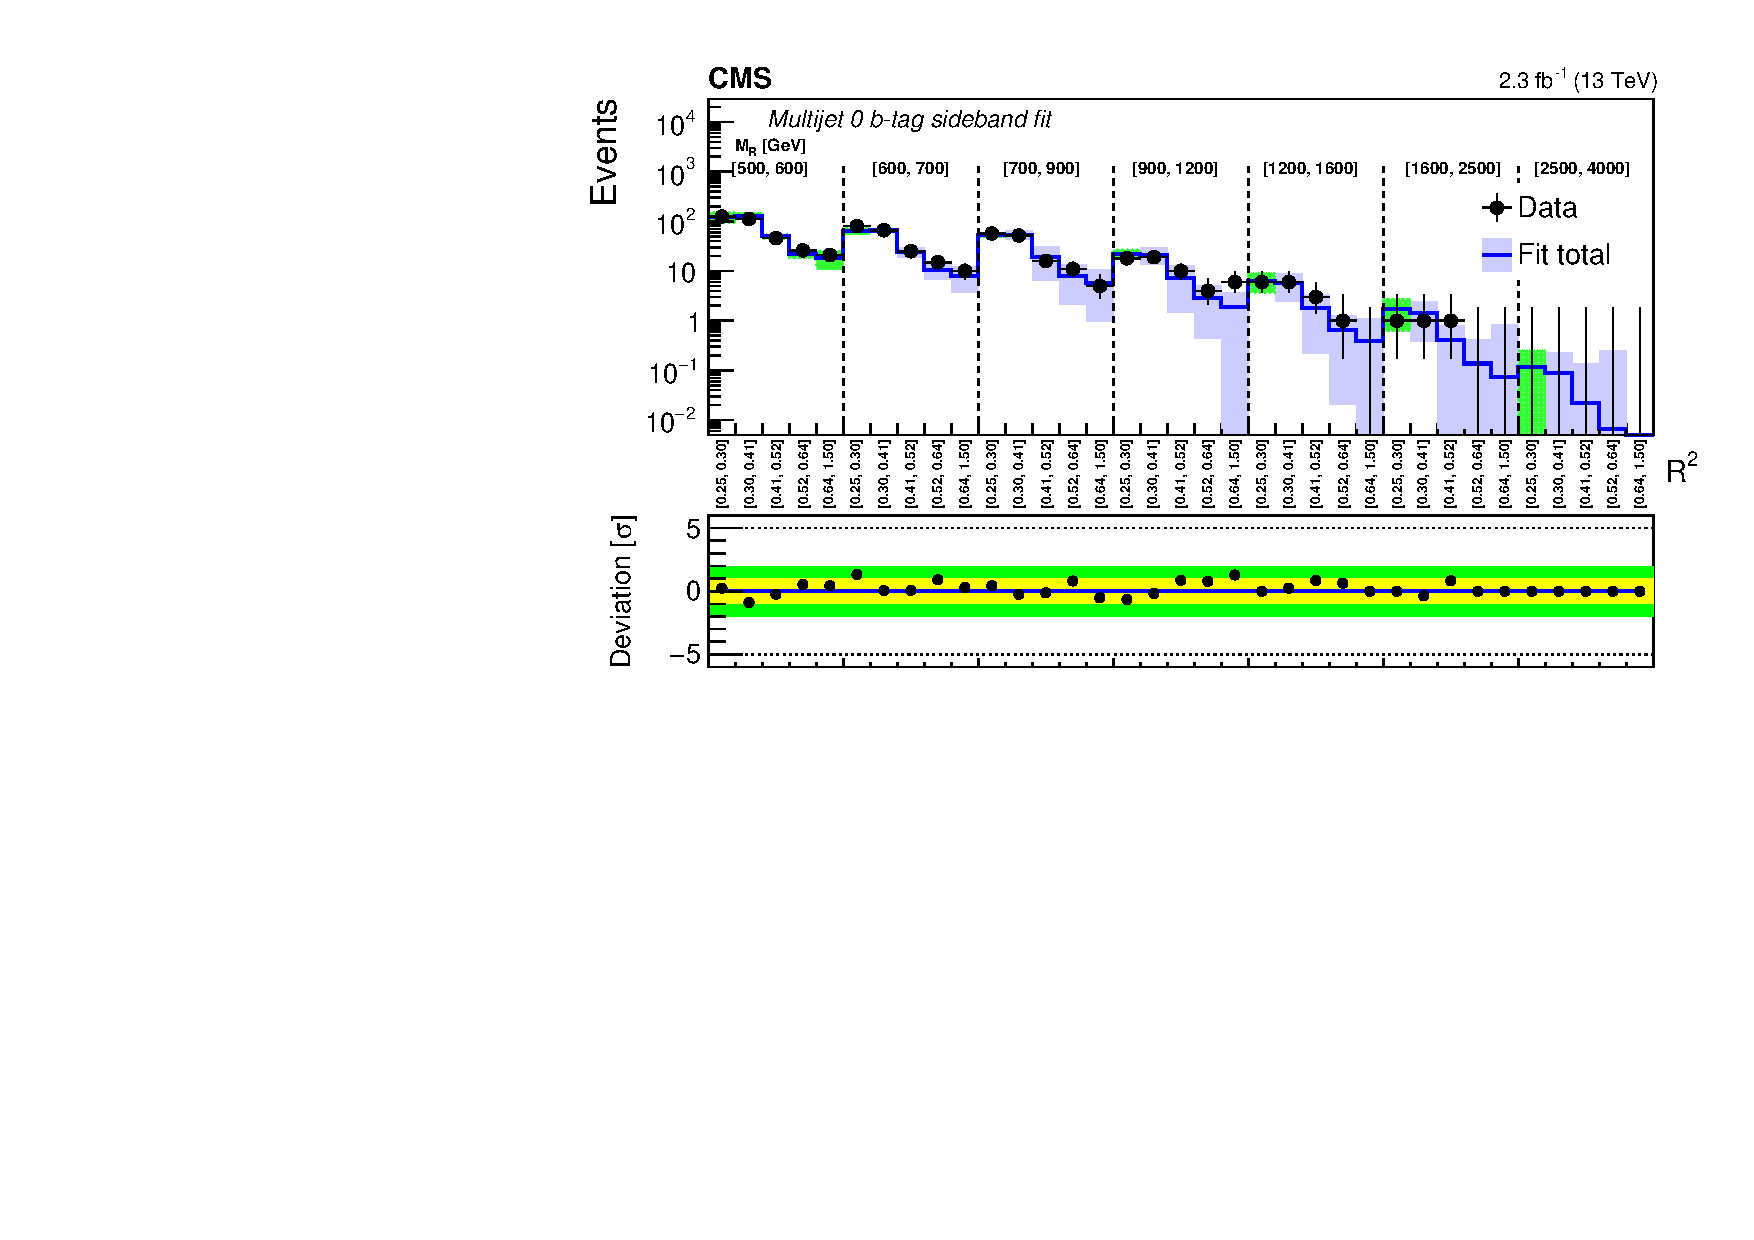
\includegraphics[width=0.9\textwidth]{figs/analysis13TeV/results/h_th1x_ns_0btag_MultiJet.pdf}}\\
\subfigure{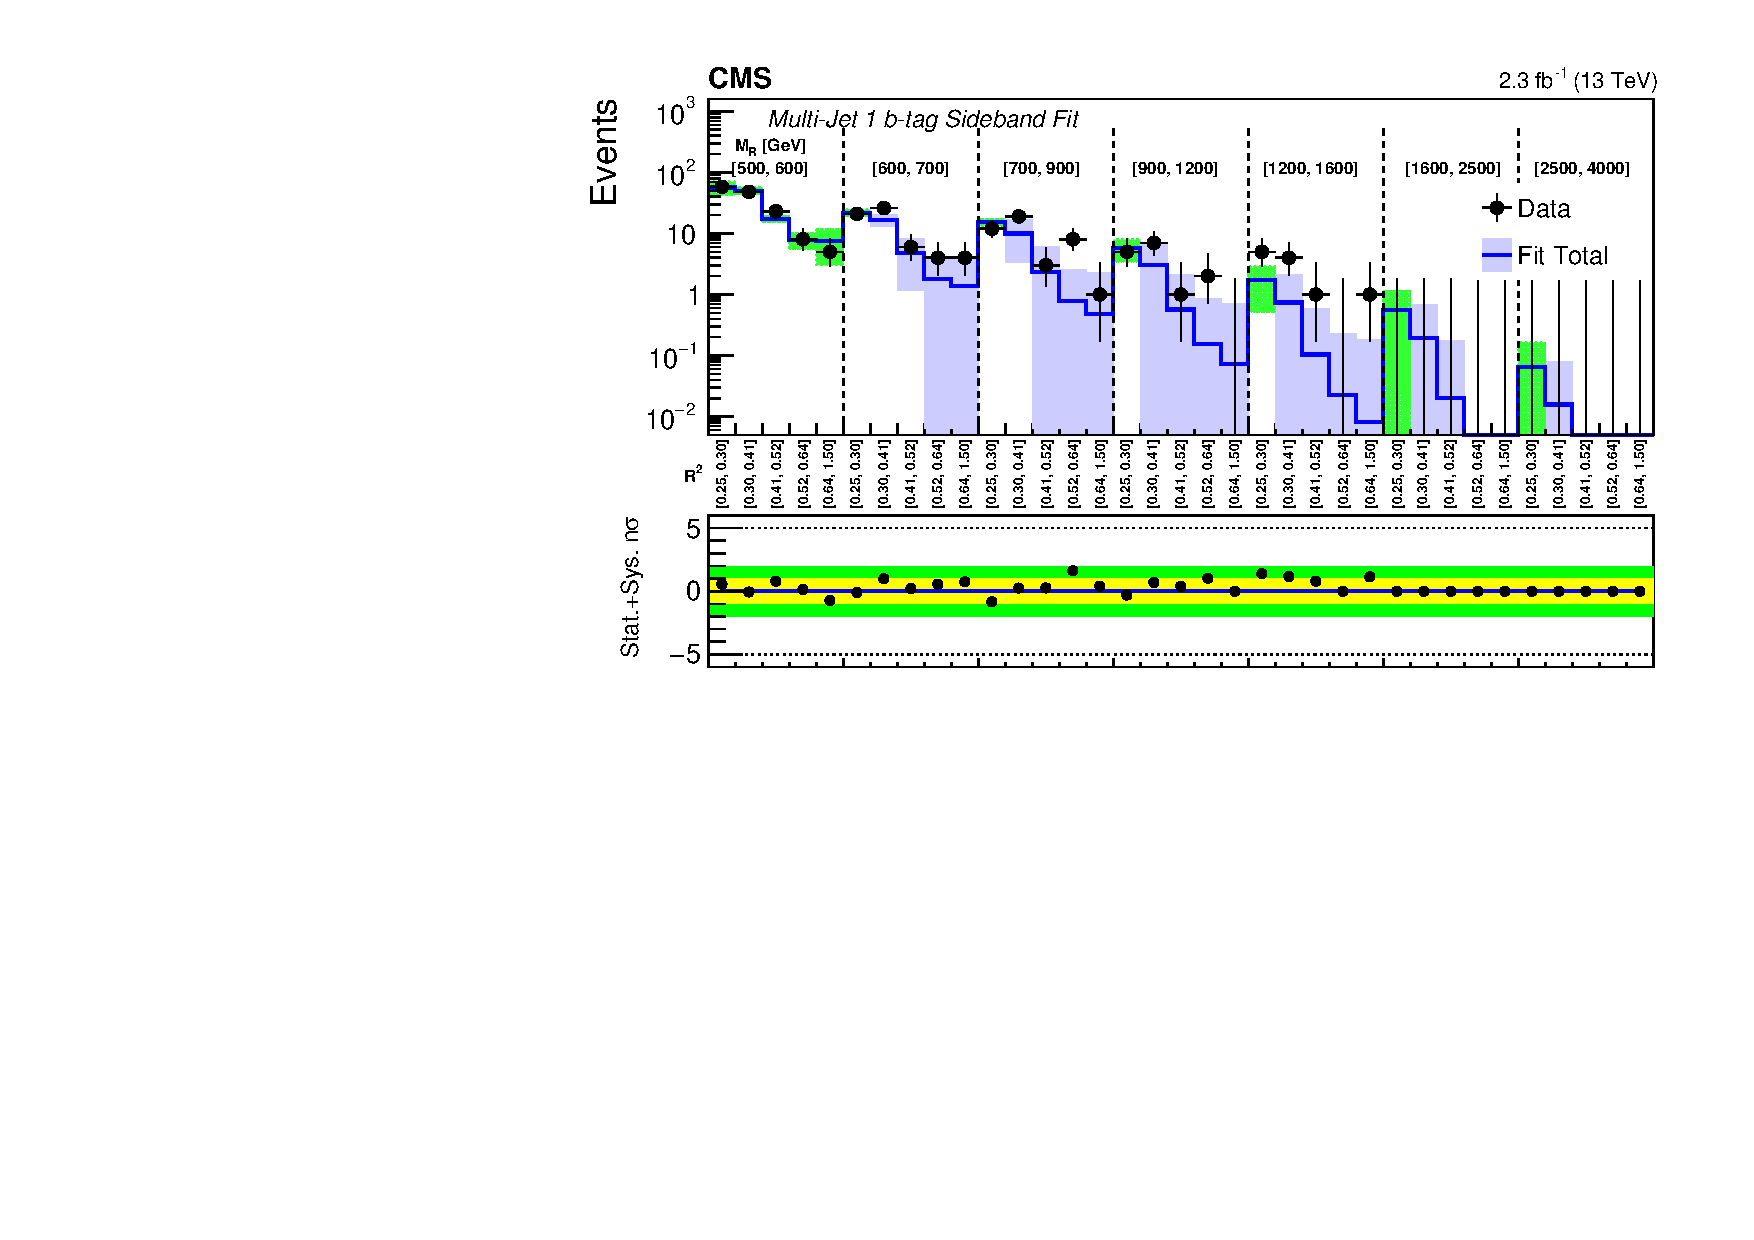
\includegraphics[width=0.9\textwidth]{figs/analysis13TeV/results/h_th1x_ns_1btag_MultiJet.pdf}}
\caption{Comparison of the predicted background with the observed data
  in bins of $\MR$ and $\Rtwo$ variables in the Multijet category for
  the 0 \PQb-tag (upper) and 1 \PQb-tag (lower) bins~\cite{CMS-PAS-SUS-15-004,jmgd}. A detailed explanation of the panels is given in the caption of
  Fig.~\ref{fig:results_Multijet2btag3btag}. }
\label{fig:results_Multijet0btag1btag}
\end{figure}

\begin{figure}[!ptb] \centering
\subfigure{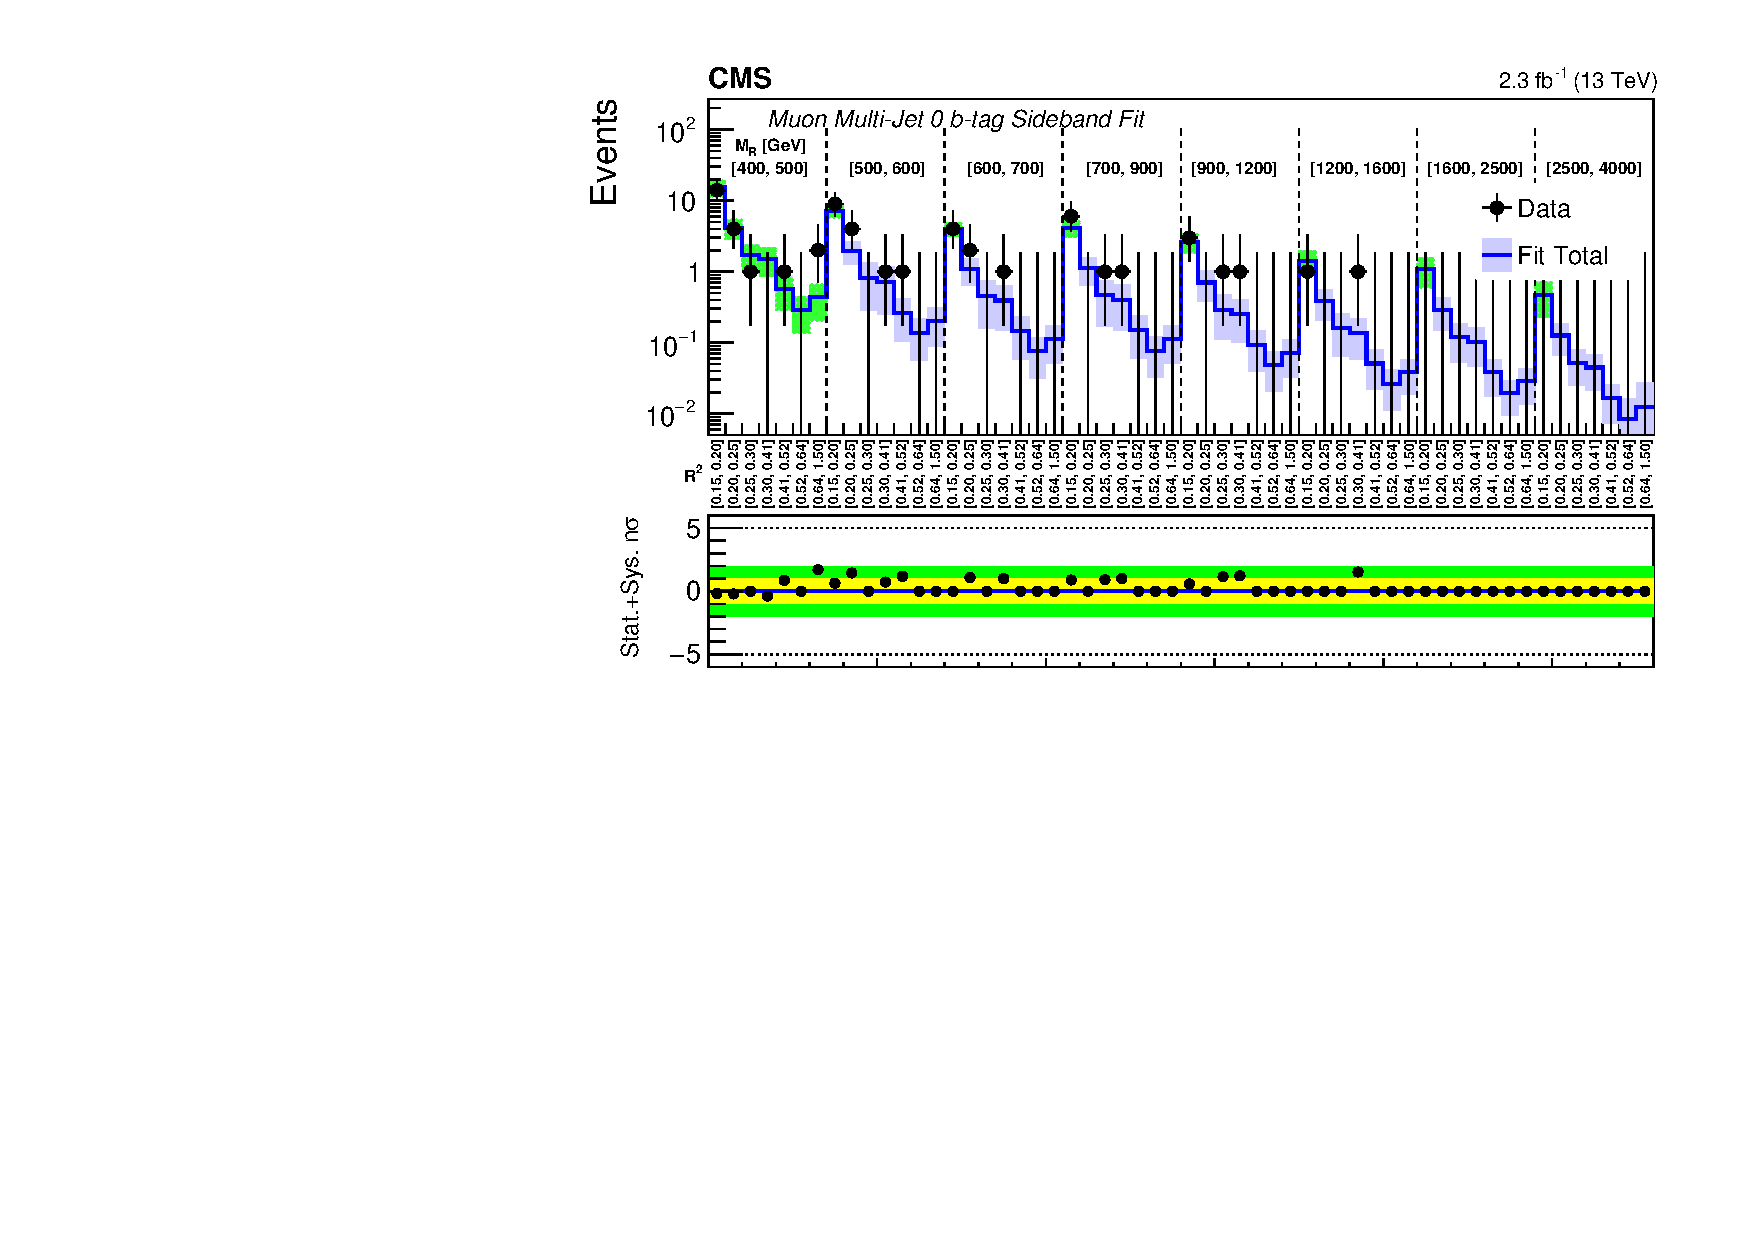
\includegraphics[width=0.9\textwidth]{figs/analysis13TeV/results/h_th1x_ns_0btag_MuMultiJet.pdf}} \\
\subfigure{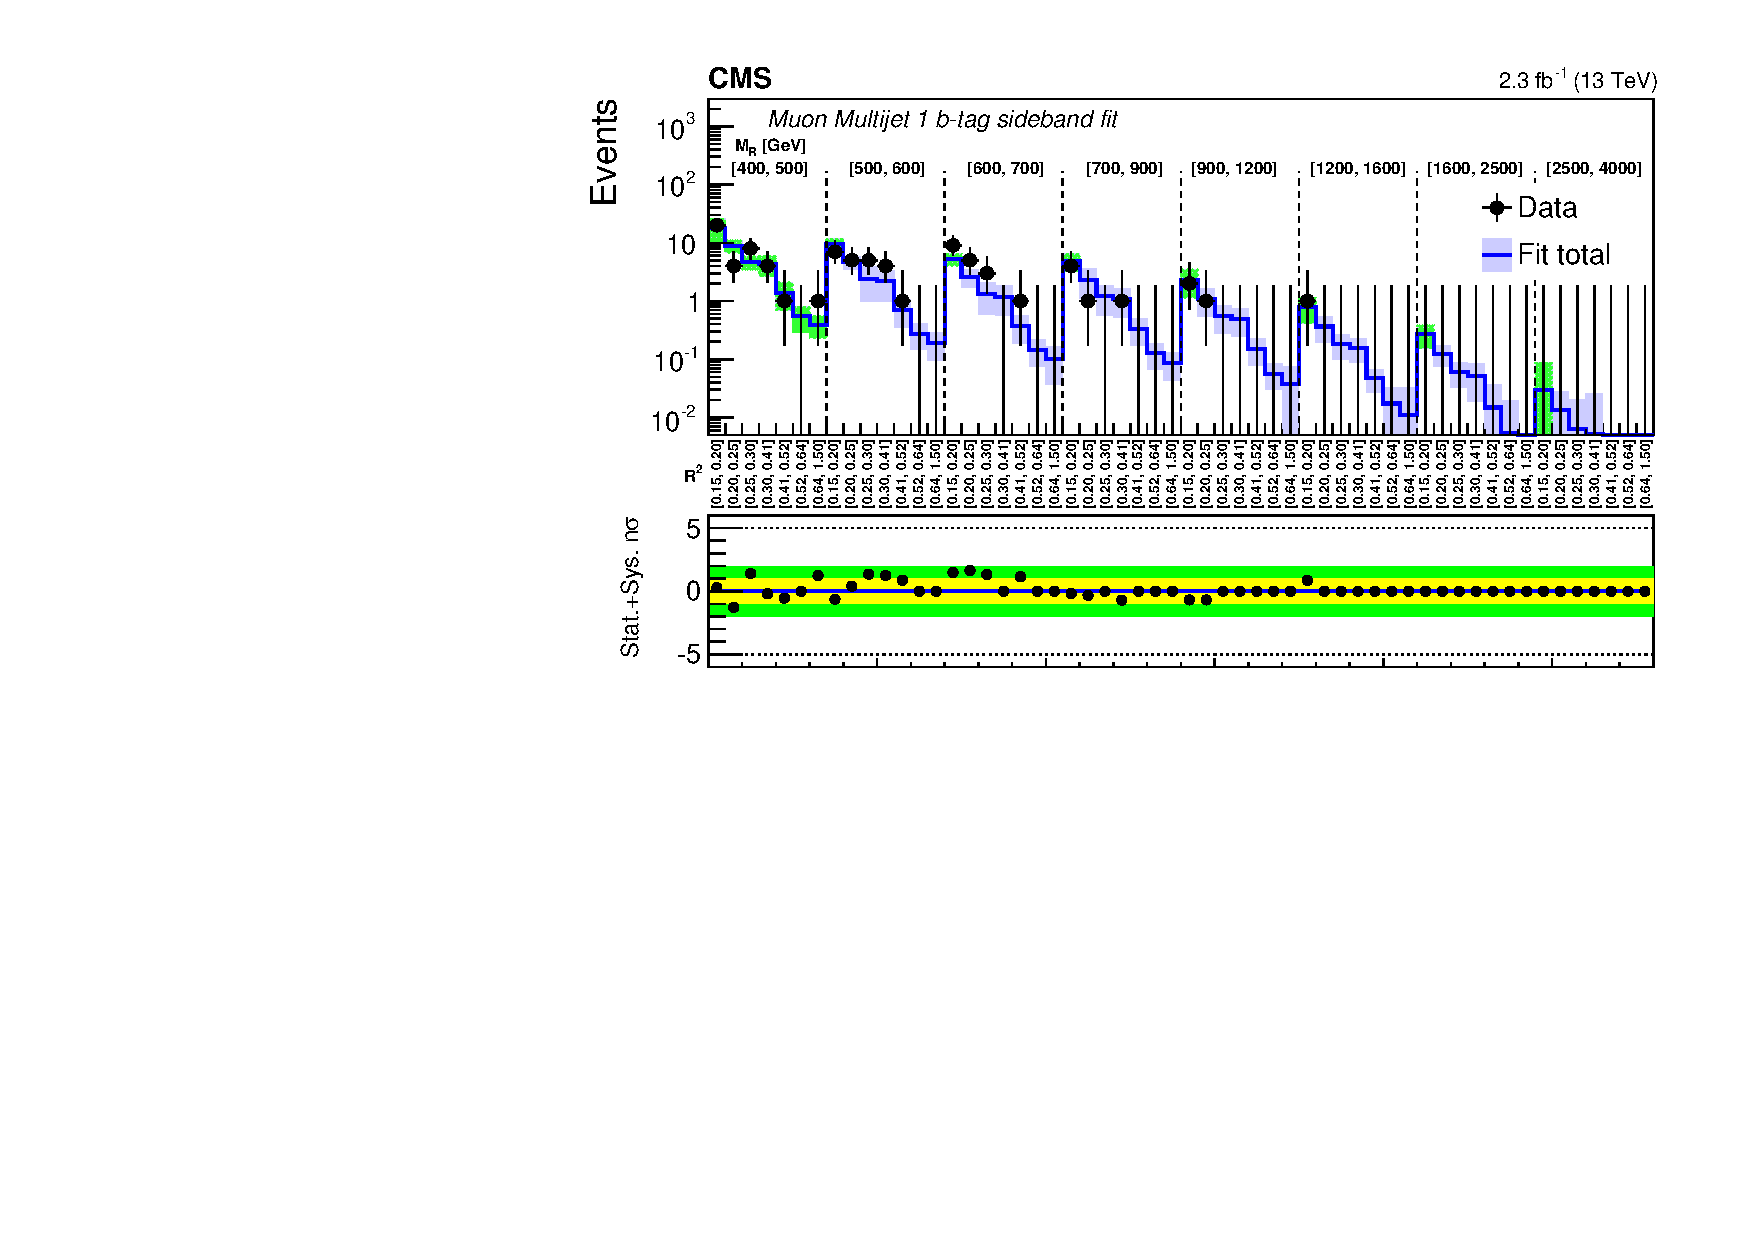
\includegraphics[width=0.9\textwidth]{figs/analysis13TeV/results/h_th1x_ns_1btag_MuMultiJet.pdf}} \\
\caption{Comparison of the predicted background with the observed data
  in bins of $\MR$ and $\Rtwo$ variables in the Muon Multijet
  category for the 0 \PQb-tag (upper) and 1 \PQb-tag (lower) bins~\cite{CMS-PAS-SUS-15-004,jmgd}. A detailed explanation of the panels is given in the caption of
  Fig.~\ref{fig:results_Multijet2btag3btag}. }
\label{fig:results_MuMultijet0btag1btag}
\end{figure}

\begin{figure}[!ptb] \centering
\subfigure{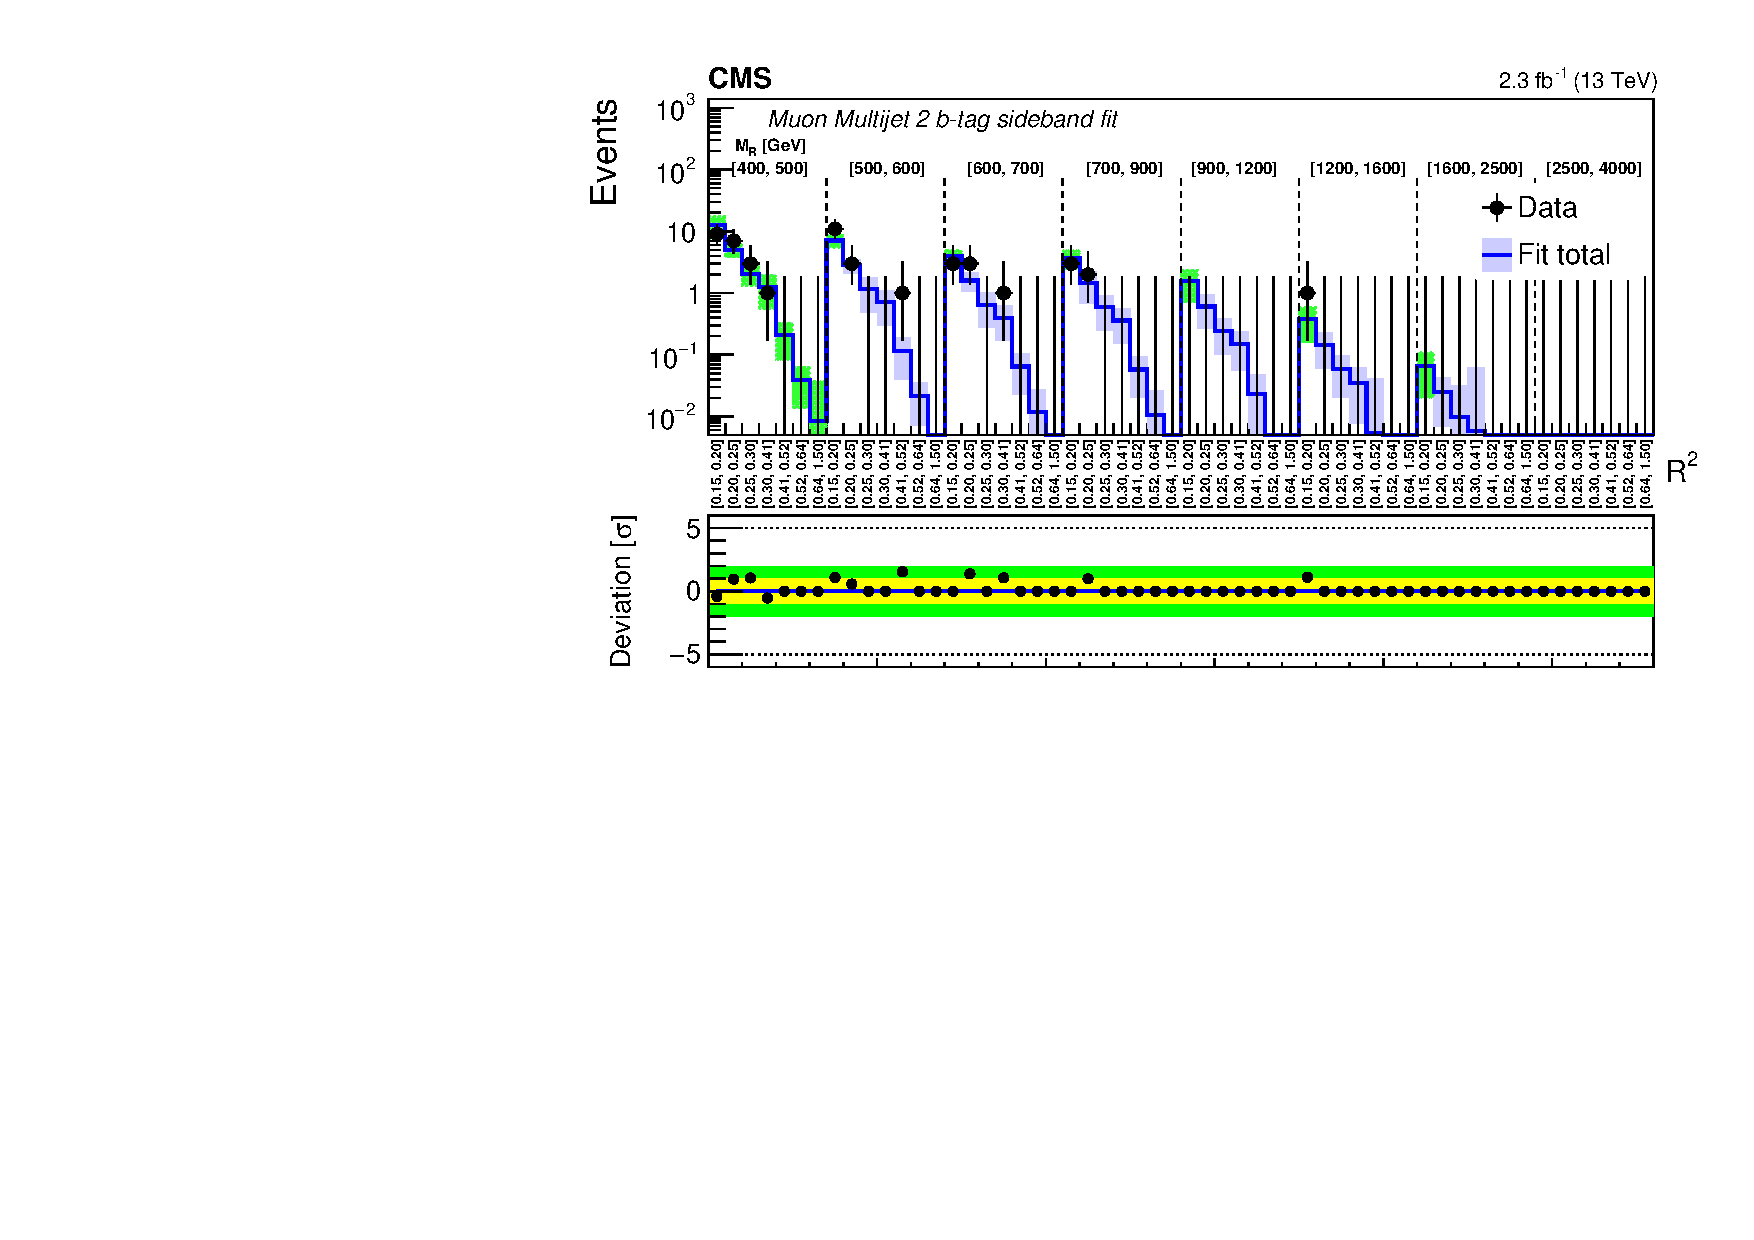
\includegraphics[width=0.9\textwidth]{figs/analysis13TeV/results/h_th1x_ns_2btag_MuMultiJet.pdf}} \\
\subfigure{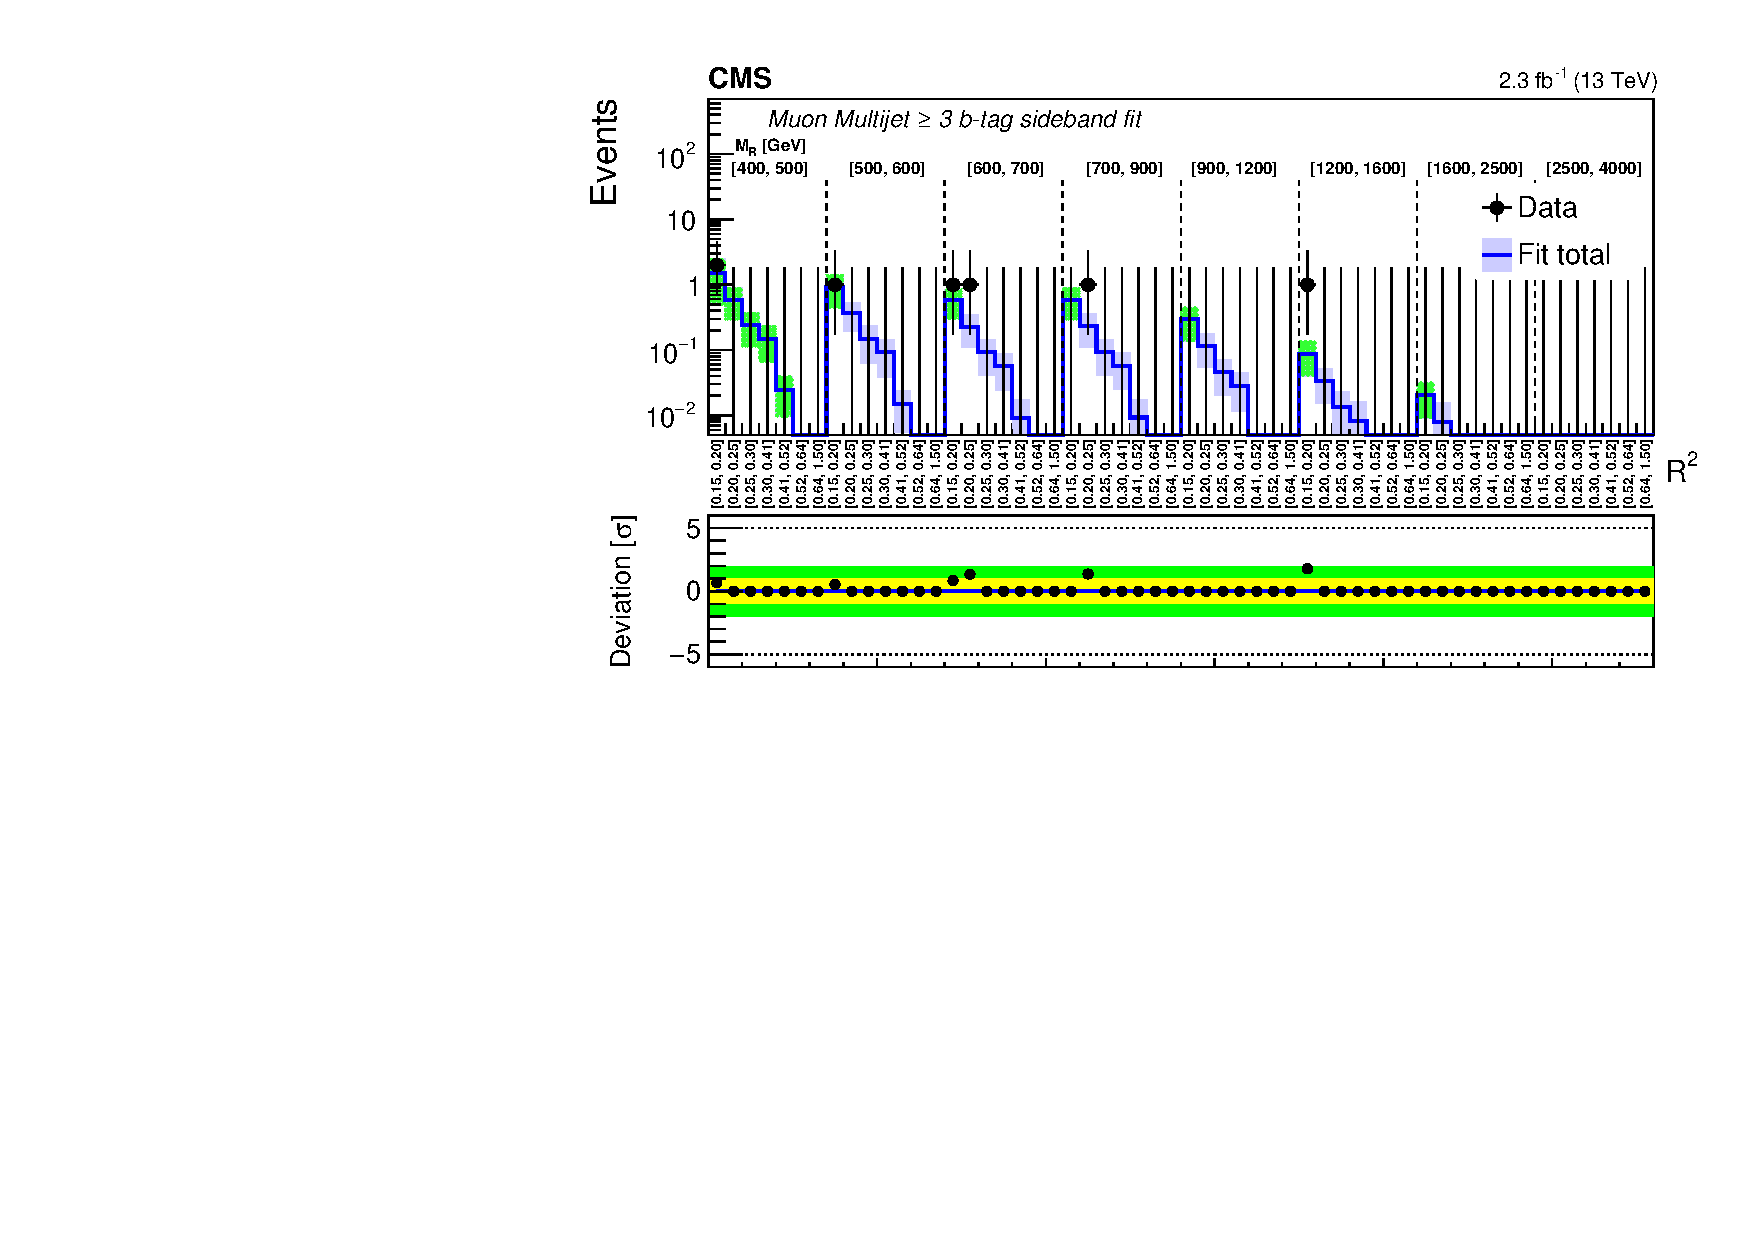
\includegraphics[width=0.9\textwidth]{figs/analysis13TeV/results/h_th1x_ns_3btag_MuMultiJet.pdf}}
\caption{Comparison of the predicted background with the observed data
  in bins of $\MR$ and $\Rtwo$ variables in the Muon Multijet
  category for the 2 \PQb-tag (upper) and $\geq 3$ \PQb-tag (lower) bins~\cite{CMS-PAS-SUS-15-004,jmgd}. A detailed explanation of the panels is given in the caption of
  Fig.~\ref{fig:results_Multijet2btag3btag}. }
\label{fig:results_MuMultijet2btag3btag}
\end{figure}

\begin{figure}[!ptb] \centering
\subfigure{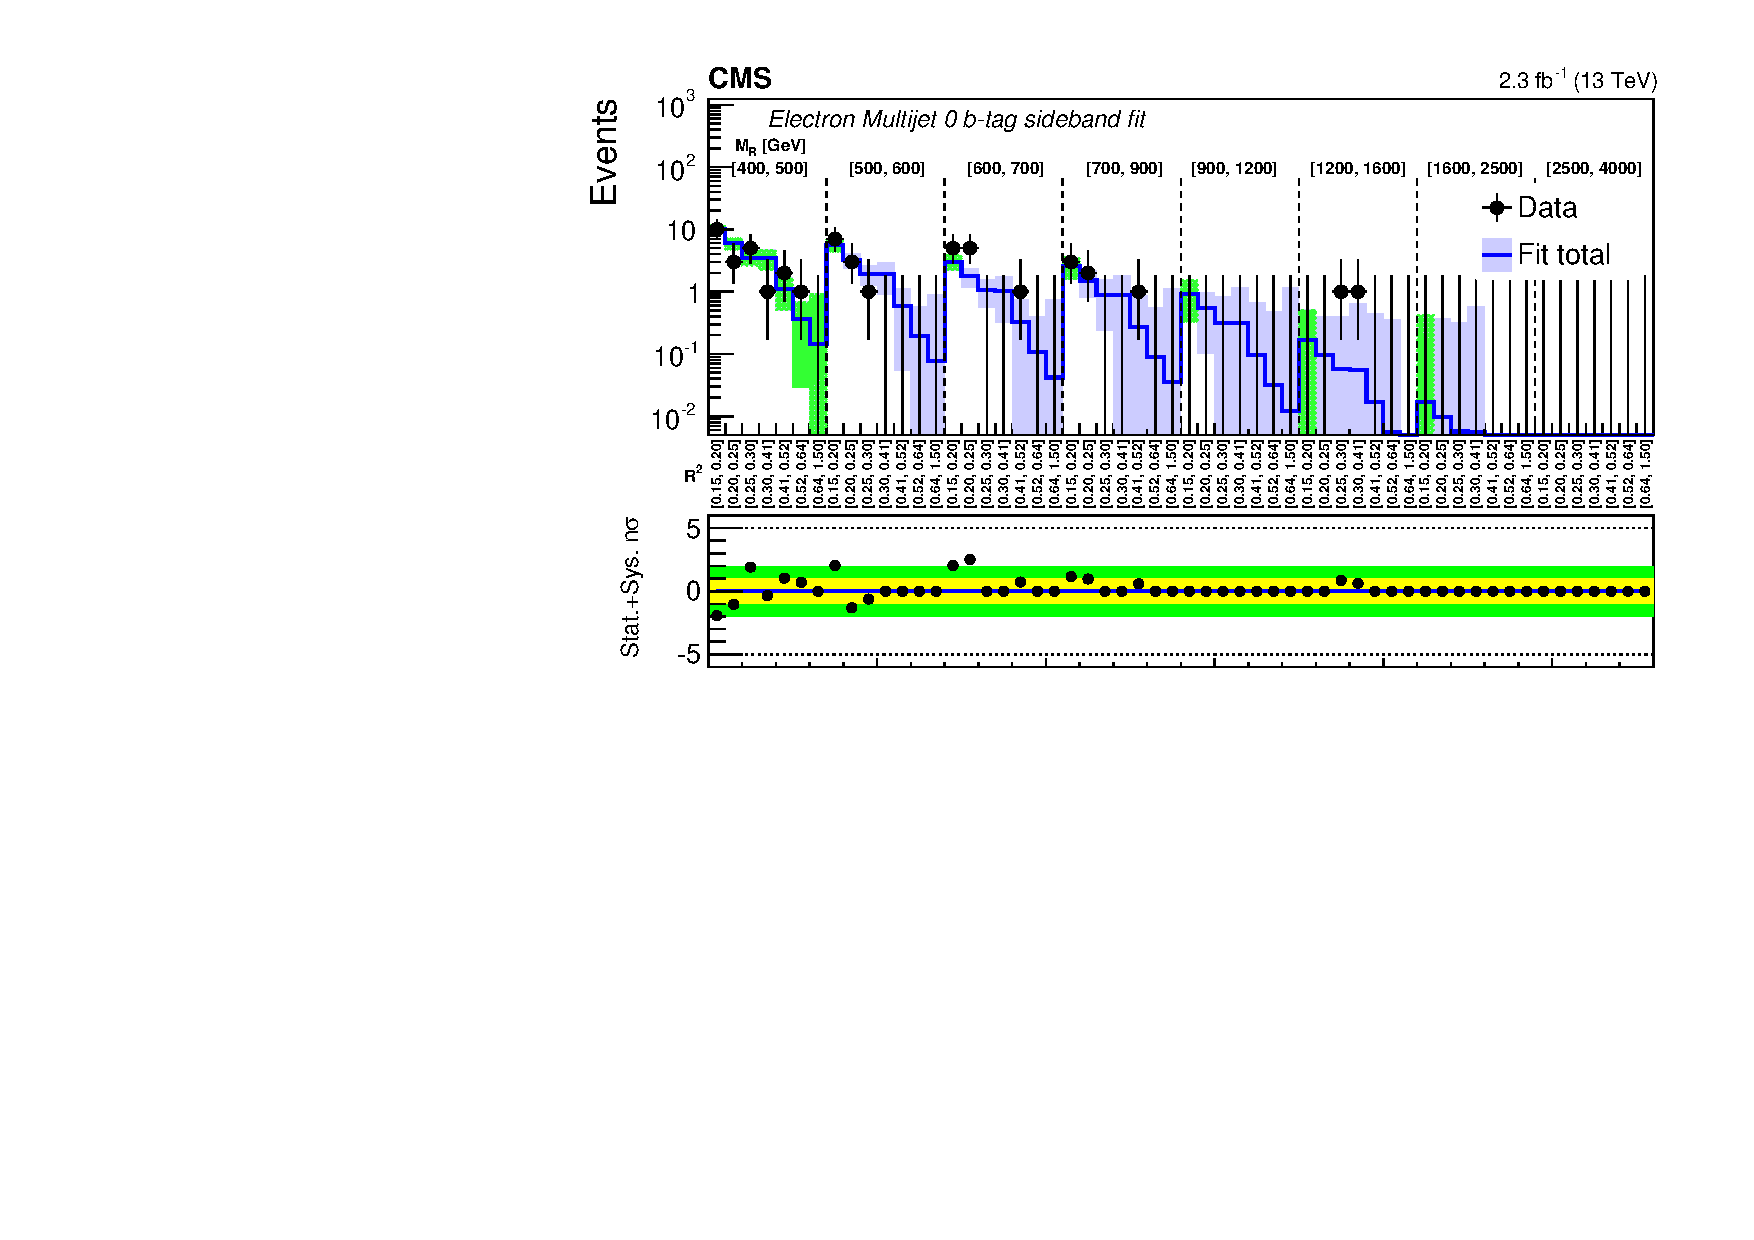
\includegraphics[width=0.9\textwidth]{figs/analysis13TeV/results/h_th1x_ns_0btag_EleMultiJet.pdf}} \\
\subfigure{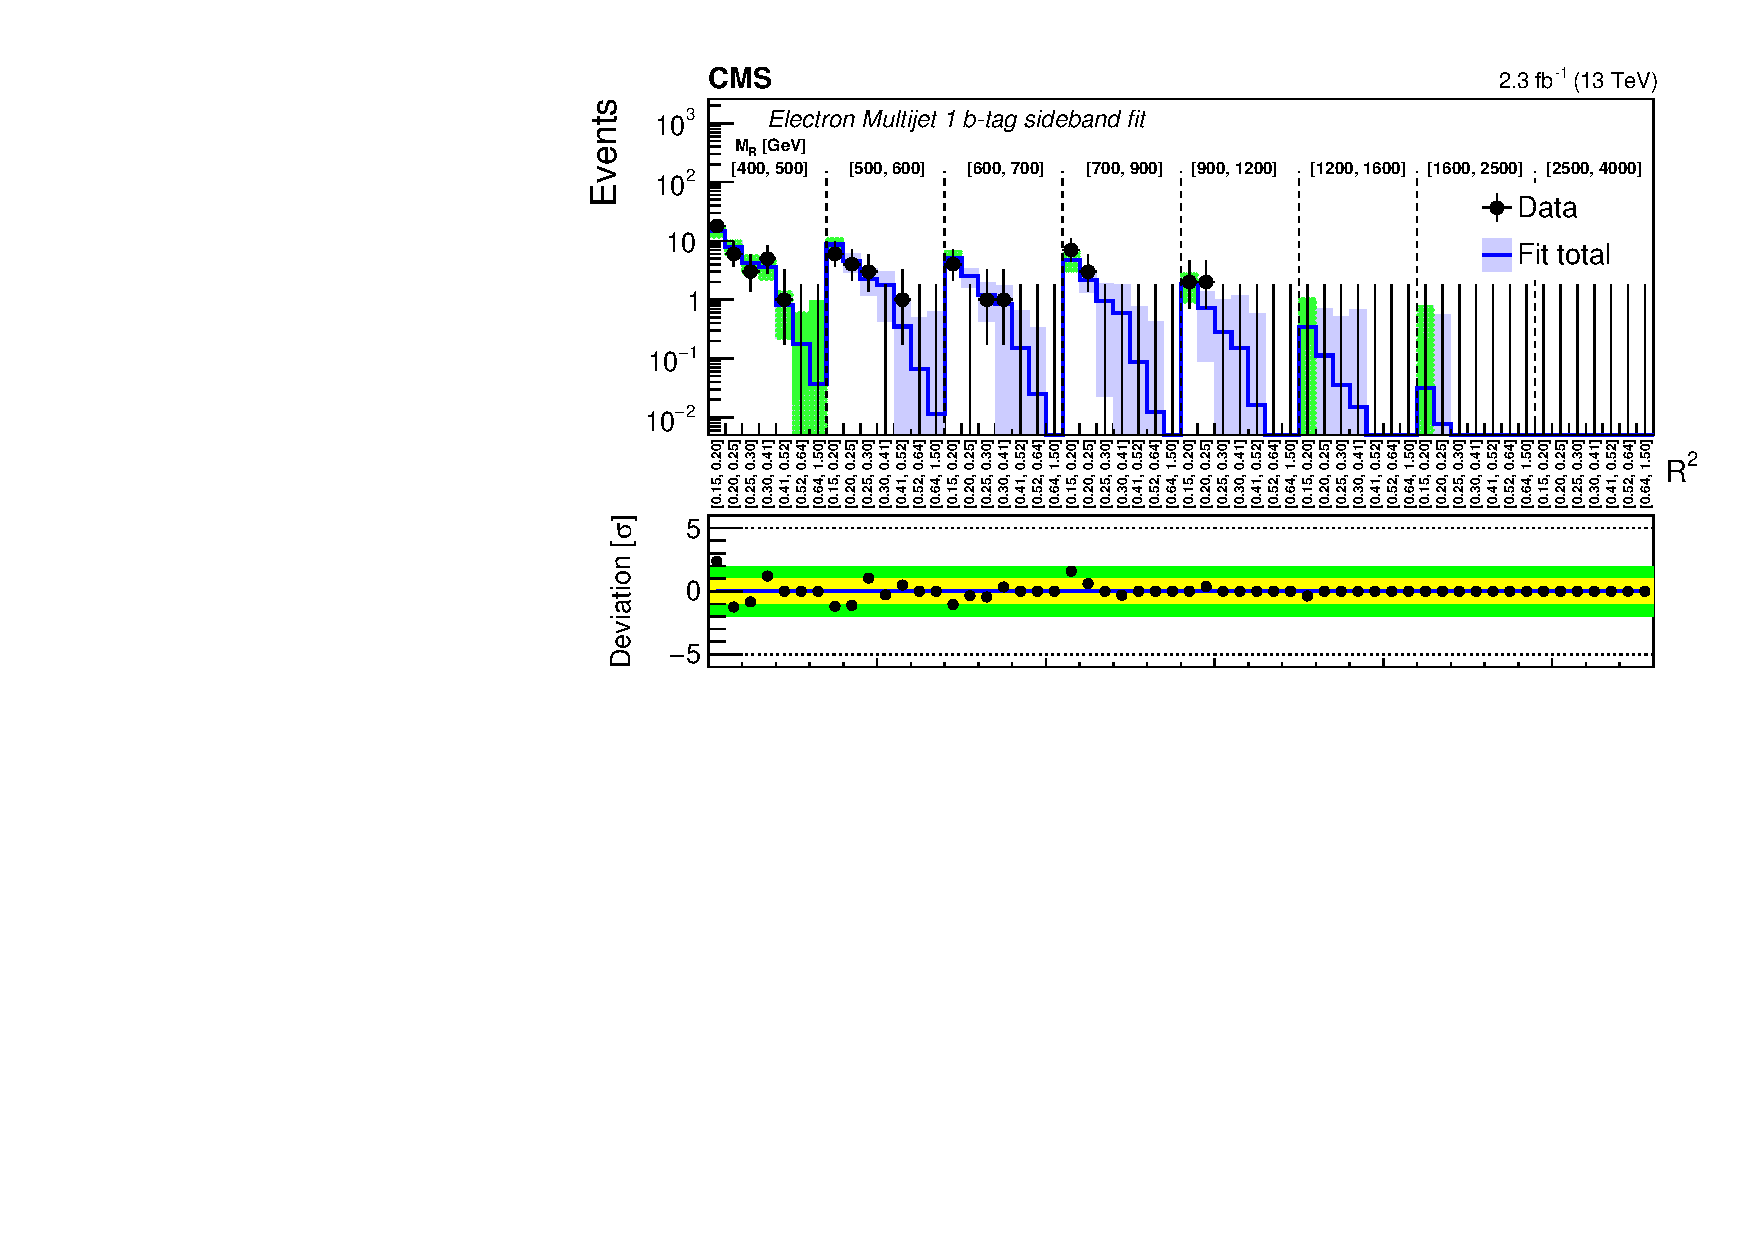
\includegraphics[width=0.9\textwidth]{figs/analysis13TeV/results/h_th1x_ns_1btag_EleMultiJet.pdf}} 
\caption{Comparison of the predicted background with the observed data
  in bins of $\MR$ and $\Rtwo$ variables in the Electron Multijet
  category for the 0 \PQb-tag (upper) and 1 \PQb-tag (lower) bins~\cite{CMS-PAS-SUS-15-004,jmgd}. A detailed explanation of the panels is given in the caption of
  Fig.~\ref{fig:results_Multijet2btag3btag}. }
\label{fig:results_EleMultijet0btag1btag}
\end{figure}

\begin{figure}[!ptb] \centering
\subfigure{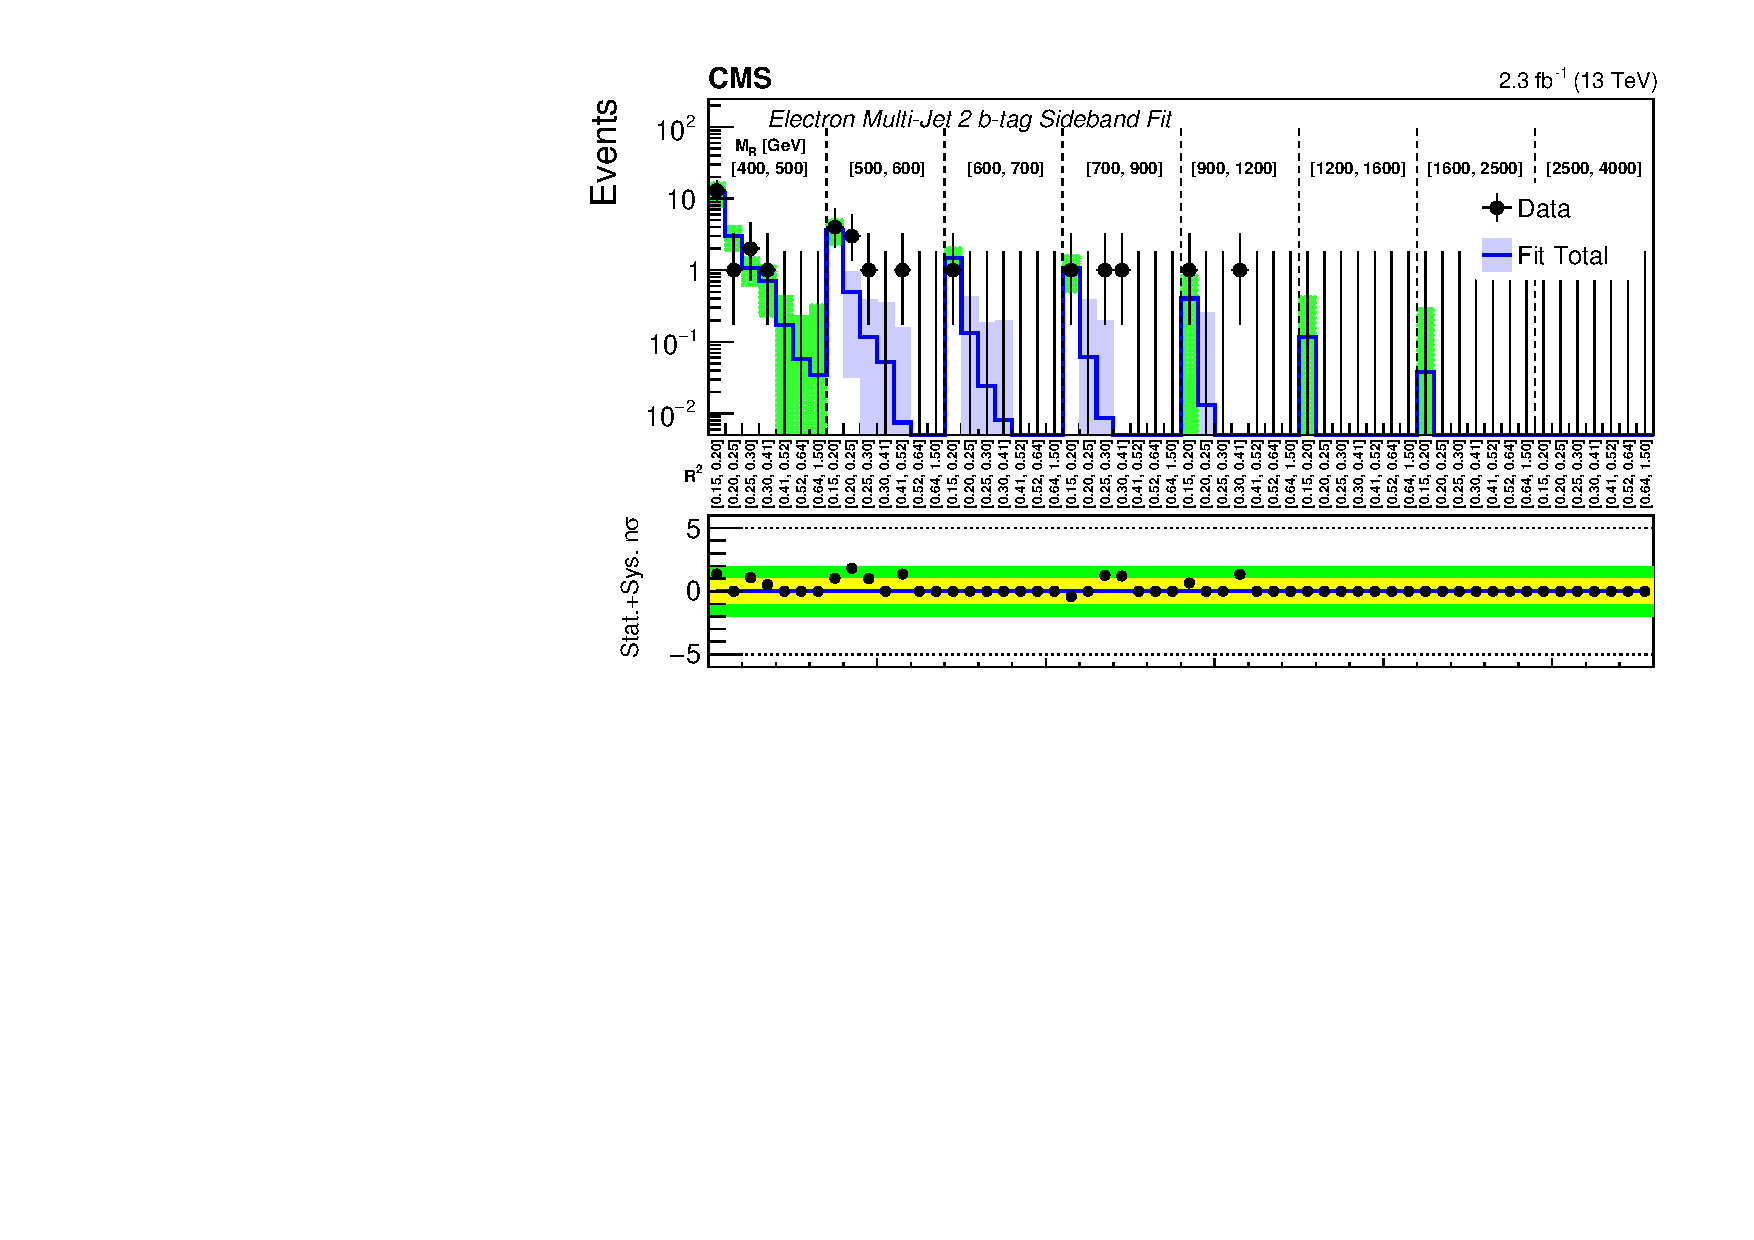
\includegraphics[width=0.9\textwidth]{figs/analysis13TeV/results/h_th1x_ns_2btag_EleMultiJet.pdf}} \\
\subfigure{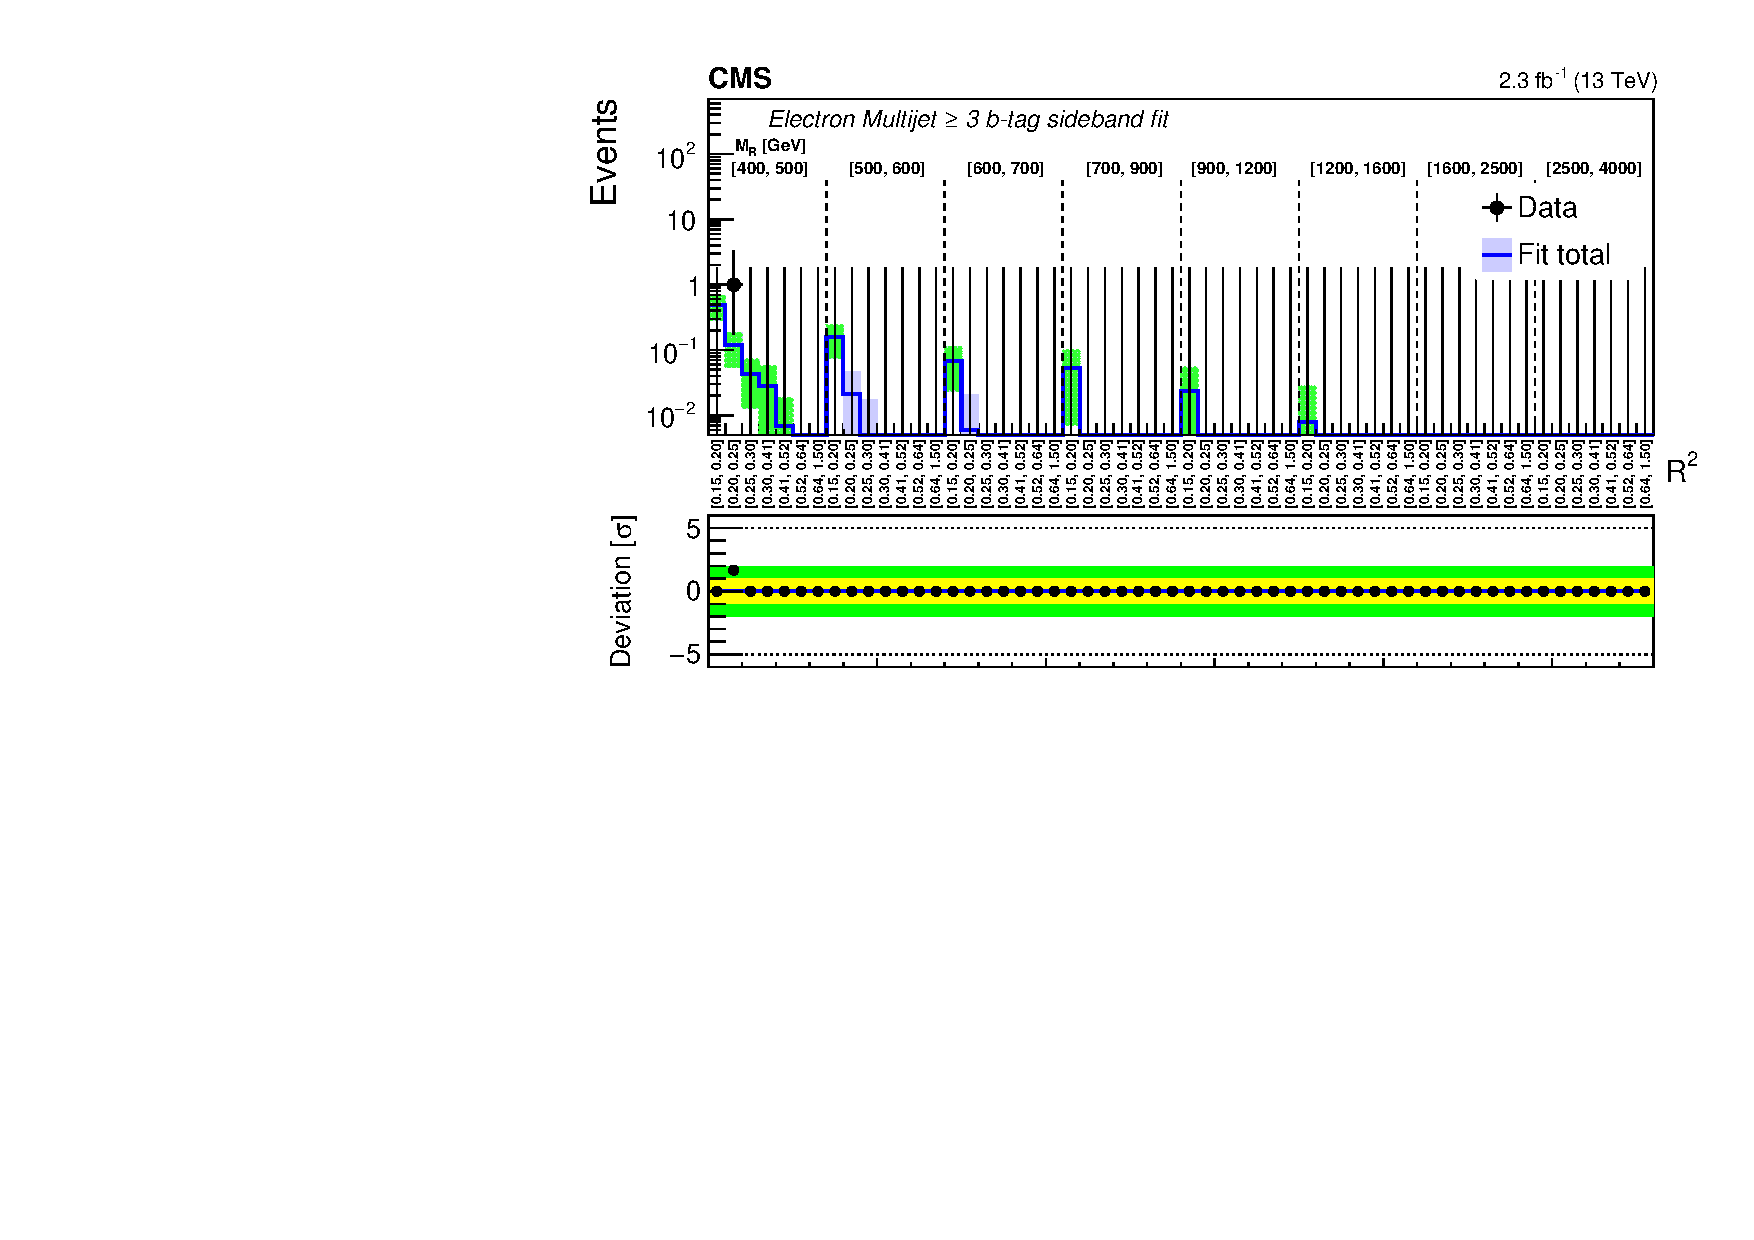
\includegraphics[width=0.9\textwidth]{figs/analysis13TeV/results/h_th1x_ns_3btag_EleMultiJet.pdf}}
\caption{Comparison of the predicted background with the observed data
  in bins of $\MR$ and $\Rtwo$ variables in the Electron Multijet
  category for the 2 \PQb-tag (upper) and $\geq 3$ \PQb-tag (lower) bins~\cite{CMS-PAS-SUS-15-004,jmgd}. A detailed explanation of the panels is given in the caption of
  Fig.~\ref{fig:results_Multijet2btag3btag}. }
\label{fig:results_EleMultijet2btag3btag}
\end{figure}

\clearpage

\subsection{Comparison of the two methods}

The background predictions obtained from methods A and B are systematically compared 
in all of the search region categories. For method B, the model-independent 
fit to the sideband is used for this comparison. In Fig.~\ref{fig:FitVsMADD},
we show the comparison of the two background predictions for two example event categories.
The predictions from the two methods agree within the uncertainties of each method.
The uncertainty from the fit-based method tends to be slightly larger at high
$\MR$ and $\Rtwo$ due to the additional uncertainty in the exact shape of 
the tail of the distribution, as the $n$ and $b$ parameters are not strongly 
constrained by the sideband data. 

\begin{figure}[!htb] \centering
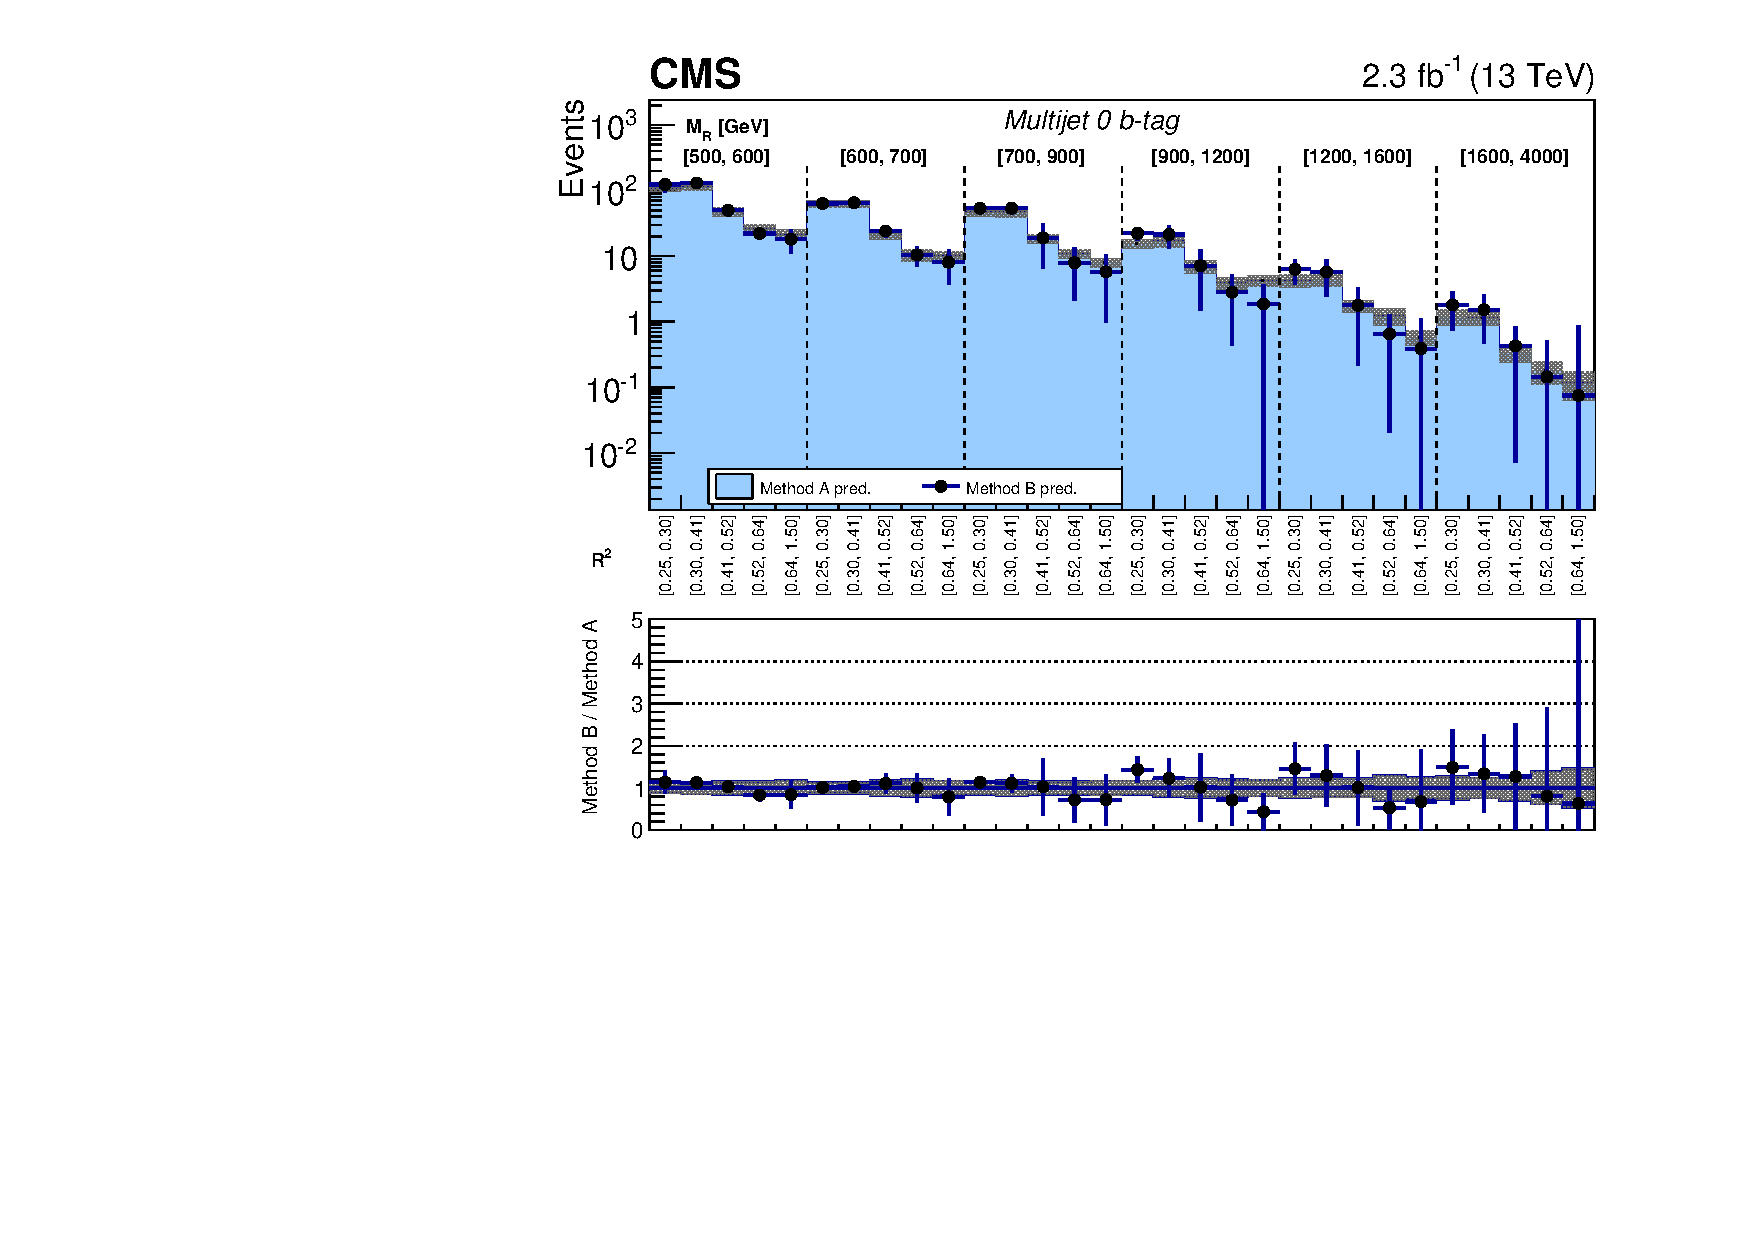
\includegraphics[width=0.9\textwidth]{figs/analysis13TeV/results/MRRsqMultiJet0BTagMCTotalUnrolledMCFit.pdf}
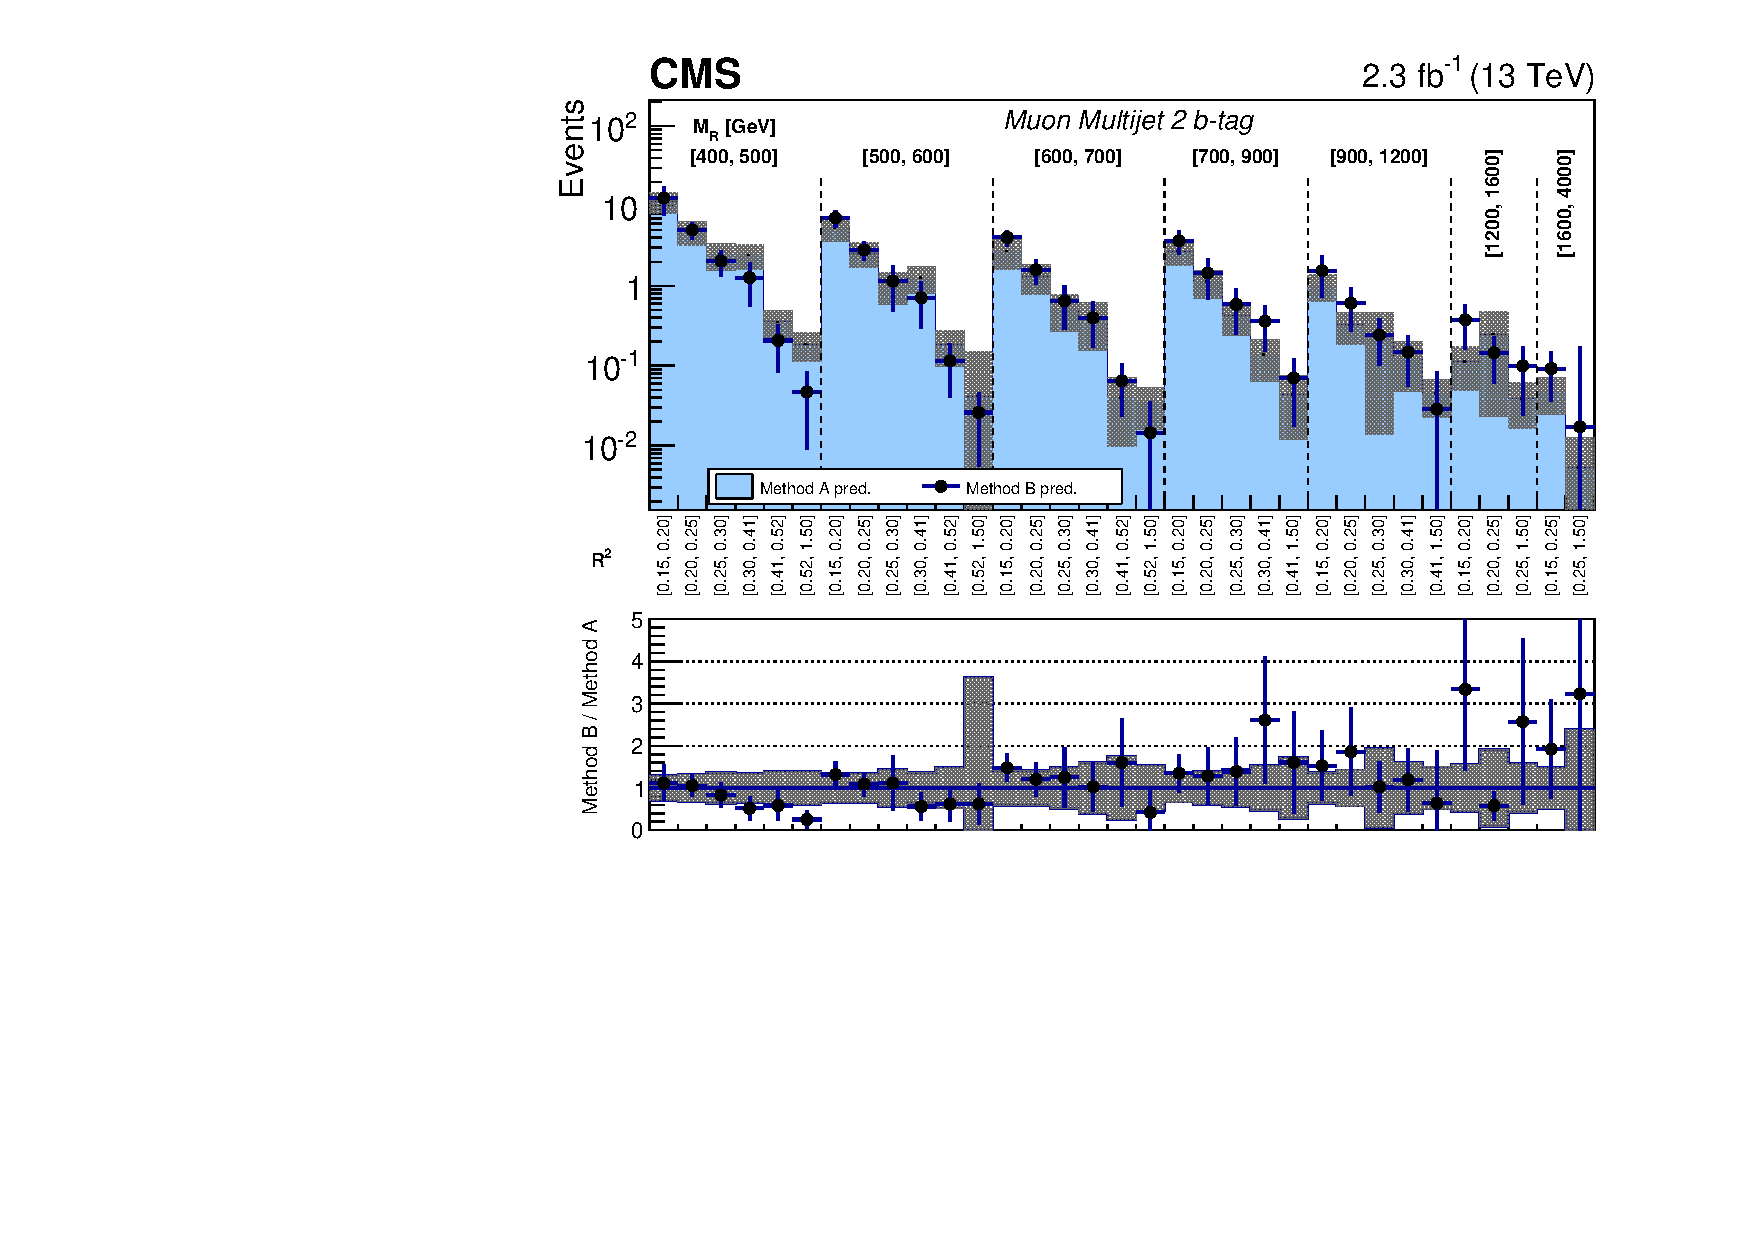
\includegraphics[width=0.9\textwidth]{figs/analysis13TeV/results/MRRsqMuMultiJet2BTagMCTotalUnrolledMCFit.pdf}
\caption{Comparisons of the two alternative background predictions for the ($\MR$,$\Rtwo$) distribution 
for the 0 \PQb-tag bin of the Multijet category (upper) and the 2 \PQb-tag bin of the Muon Multijet
category (lower)~\cite{CMS-PAS-SUS-15-004}. The two-dimensional ($\MR$,$\Rtwo$) distribution is shown
in a one-dimensional representation, with each $\MR$ bin marked by the dashed lines and labeled near the top
and each $\Rtwo$ bin labeled below. The ratios of the method B fit-based predictions to the method A simulation-assisted predictions are shown
on the bottom panels. The method B uncertainty is represented by the error bars on the data points and the
method A uncertainty is represented by the shaded region. 
} 
\label{fig:FitVsMADD}
\end{figure}

The two background predictions use methods based on data that make 
very different systematic assumptions. Method A assumes that corrections
to the simulation prediction measured in control regions apply also to the
signal regions, while method B assumes that the shape of the background distribution
in $\MR$ and $\Rtwo$ is well described by a particular exponentially falling functional 
form. The agreement observed between predictions obtained using these two very different 
methods significantly enhances the confidence of the background modeling, and 
also validates the respective assumptions.

\clearpage

\section{Systematic uncertainties}
\label{sec:Systematics}

Various systematic uncertainties are considered in the evaluation of the
signal and background predictions. Different types of systematic
uncertainties are considered for the two different background models.

For method A, the largest uncertainties arise from the precision with
which the MC corrections are measured. The dominant uncertainties
in the correction factors result from statistical uncertainties due to 
the limited size of the control region event sample. We also propagate systematic
uncertainties in the theoretical cross-section for the small residual backgrounds 
present in the control regions, and they contribute $2-5\%$ to the 
correction factor uncertainty. 
Additional systematic uncertainties are computed from the procedure that
tests that the accuracy of the MC corrections as a function of 
($\MR$, $\Rtwo$), and the number of \PQb-tagged jets in events with four or more jets. 
The total uncertainty from this procedure ranges from $10\%$ for the most populated bins to
$50\%$ and $100\%$ for the least populated bins. For the $\cPZ\rightarrow\nu\bar\nu$ process, we 
also propagate the difference in the correction factors measured in the three alternative 
control regions as a systematic uncertainty, intended to estimate the possible differences in 
the simulation mismodeling of the hadronic recoil for the $\cPgg+$jets process and 
the $\cPZ(\nu\bar\nu)+$jets process. These systematic uncertainties 
range from $10$ to $40\%$. For the QCD background prediction the statistical uncertainty 
due to limited event counts in the $\dPhiR>2.8$ control regions and the systematic
uncertainty of $87\%$ in the translation factor $\zeta$ are propagated.

For method B, the systematic uncertainties in the background are propagated as part of 
the maximum likelihood fit procedure. For each event category, the background shape in 
$\MR$ and $\Rtwo$ is described by four independent parameters: two 
that control the exponential fall off and two that control the behavior of the
nonexponential tail. Systematic uncertainties in the background are propagated 
through the profiling of these unconstrained shape parameters. For more populated bins, such as 
the 0 \PQb-tag and 1 \PQb-tag bins in the Multijet category, the systematic uncertainties range from
about 30\% at low $\MR$ and $\Rtwo$ to about 70\% at high $\MR$ and $\Rtwo$.
For sparsely populated bins such as the 3-or-more \PQb-tag bin in the Muon Multijet or Electron
Multijet categories, the systematic uncertainties range from
about 60\% at low $\MR$ and $\Rtwo$ to more than 200\% at high $\MR$ and $\Rtwo$.

\begin{table}[!htb]\centering
\caption{Summary of the main instrumental and theoretical systematic
  uncertainties. The systematic uncertainty associated to the modeling
  of the initial-state radition is only applied for events with recoil above $400\GeV$.}
\label{tab:BackgroundSystematics}
\resizebox{\textwidth}{!}{
\begin{tabular}{ccc}
\hline\hline
Source      & On signal and/or bkg   & Typical values [\%] \\ \hline
Jet energy scale                   & Both                   & $2-15$ \\ 
Electron energy scale              & Both                   & $7-9$ \\
Muon momentum scale                & Both                   & $7-9$ \\ 
Muon efficiency                    & Both                   & $7-8$ \\
Electron efficiency                & Both                   & $7-8$ \\
Trigger efficiency                 & Both                   & $3$ \\ 
\PQb-tagging  efficiency           & Both                   & $6-15$ \\ 
\PQb mistagging  efficiency        & Both                   & $4-7$ \\ 
Missing higher orders            & Both                   & $10-25$ \\
Integrated luminosity                         & Both                   & $2.7$ \\
%Pileup                            & Both                   & $1\%$ \\ \hline
%Monte Carlo Statistics            & Both                   & $1/\sqrt{N_{MC}}$ \\\hline
Fast simulation corrections        & Signal only            & $0-10$ \\ 
Initial-state radiation            & Signal only            & $15-30$ \\\hline\hline
\end{tabular}}
\end{table}

Systematic uncertainties due to instrumental and theoretical effects are propagated as shape 
uncertainties in the signal predictions for methods A and B, and on the background
predictions for method A. The background prediction from method B is not affected
by these uncertainties as the shape and normalization are measured from data.
Uncertainties in the trigger and lepton selection efficiency, and the 
integrated luminosity~\cite{CMS-PAS-LUM-15-001} primarily affect the total normalization. Uncertainties in 
the \PQb-tagging efficiency affect the relative yields between different \PQb-tag categories. 
The uncertainties from missing higher-order corrections and the uncertainties in the jet 
energy and lepton momentum scale affect the shapes of the $\MR$ and $\Rtwo$ distributions.

For the signal predictions, we also propagate systematic uncertainties due to
possible inaccuracies of the fast simulation in modeling the lepton selection and 
\PQb tagging efficiencies. These uncertainties were evaluated by comparing
the $\ttbar$ and signal $\GEANT$ based MC samples with those
that used fast simulation. Finally, we propagate an uncertainty in the modeling of initial-state radiation for signal predictions, that ranges from $15\%$ for signal events with 
recoil between $400$ and $600\GeV$ to $30\%$ for events with recoil above $600\GeV$. 
The systematic uncertainties and their typical impact on the background and signal
predictions are summarized in Table~\ref{tab:BackgroundSystematics}.

\section{Interpretation}
\label{sec:Results}

We present results of the search using method A as it provides
slightly better sensitivity. The two-dimensional ($\MR$,$\Rtwo$) distributions for the search regions in the 
Multijet, Electron Multijet, and Muon Multijet categories observed in data are shown in 
Figures~\ref{fig:ResultsMultiJet0btag1btag}-\ref{fig:ResultsEleMultiJet2btag3btag},
along with the background prediction from method A. 
We observe no statistically significant discrepancies and interpret the null search
result using method A by determining the 95\%
confidence level (CL) upper limits on the production cross sections of
the SUSY models presented in Sec.~\ref{sec:sms} using a global likelihood determined by combining the
likelihoods of the different search boxes and sidebands. Following the LHC $\CLs$
procedure~\cite{LHCCLs} precisely defined in Sec.~\ref{sec:limit8TeV}, we use the profile likelihood ratio test statistic and the asymptotic
formula to evaluate the 95\% CL observed and expected limits on the SUSY
cross section $\sigma_\mathrm{NLO+NLL}$. 
Systematic uncertainties are taken into account by
incorporating nuisance parameters $\boldsymbol{\theta}$, representing different sources of
systematic uncertainty, into the likelihood function $\mathcal L(\mathrm{data}|\mu,\boldsymbol{\theta})$. 
For each signal model the simulated SUSY events are used to estimate the effect of possible signal
contamination in the analysis control regions, and the method A background prediction is corrected 
accordingly. 
As before, the template probability density for the signal, normalized
to unit probability, is multiplied by $\mu\sigma_\mathrm{NLO+NLL} L
\epsilon^{\text{box}}_{\PQb\text{-tag}}$, where $\mu$ is the signal
strength parameter, $\sigma_\mathrm{NLO+NLL}$ is
the SUSY signal cross section, $L$ is the integrated luminosity
corresponding to the size of the data set, and
$\epsilon^{\text{box}}_{\PQb\text{-tag}}$ is the signal selection
efficiency for a given category and \PQb-tagged jet multiplicity.
To determine a confidence interval for $\mu$, we construct the profile likelihood ratio test
statistic $\tilde q_{\mu}$ of Eqn.~\ref{eqn:LHCteststat} as a function of 
$\mu$. Then for example, a 68\% confidence interval for $\mu$
can be taken as the region for which the test statistic is less than 1. By
allowing each nuisance parameter to vary, the test statistic
curve is wider, reflecting the systematic uncertainty arising from
each source, and resulting in a larger confidence interval for $\mu$. 

\begin{figure}[!ptb] \centering
\subfigure{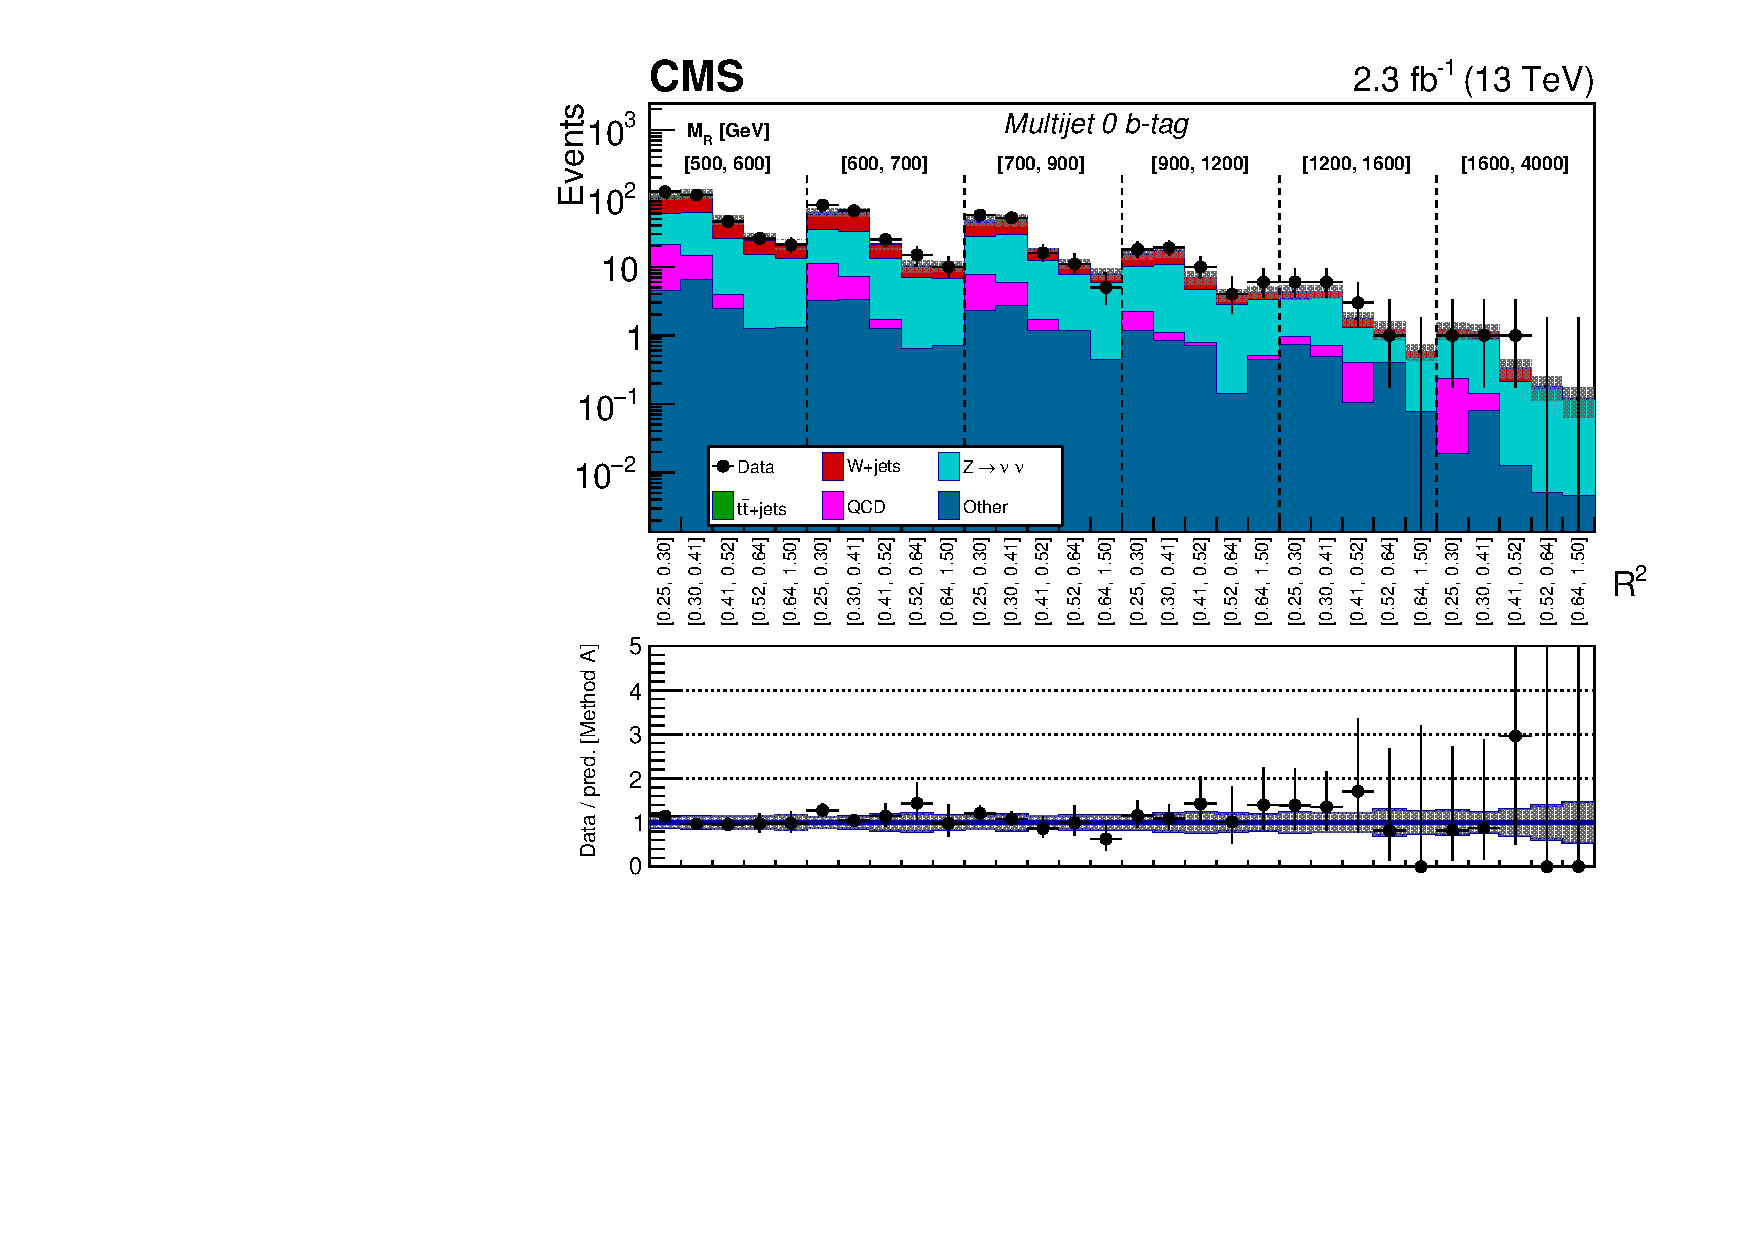
\includegraphics[width=0.8\textwidth]{figs/analysis13TeV/results/MRRsqMultiJet0BTagUnrolledDataMC.pdf}}\\
\subfigure{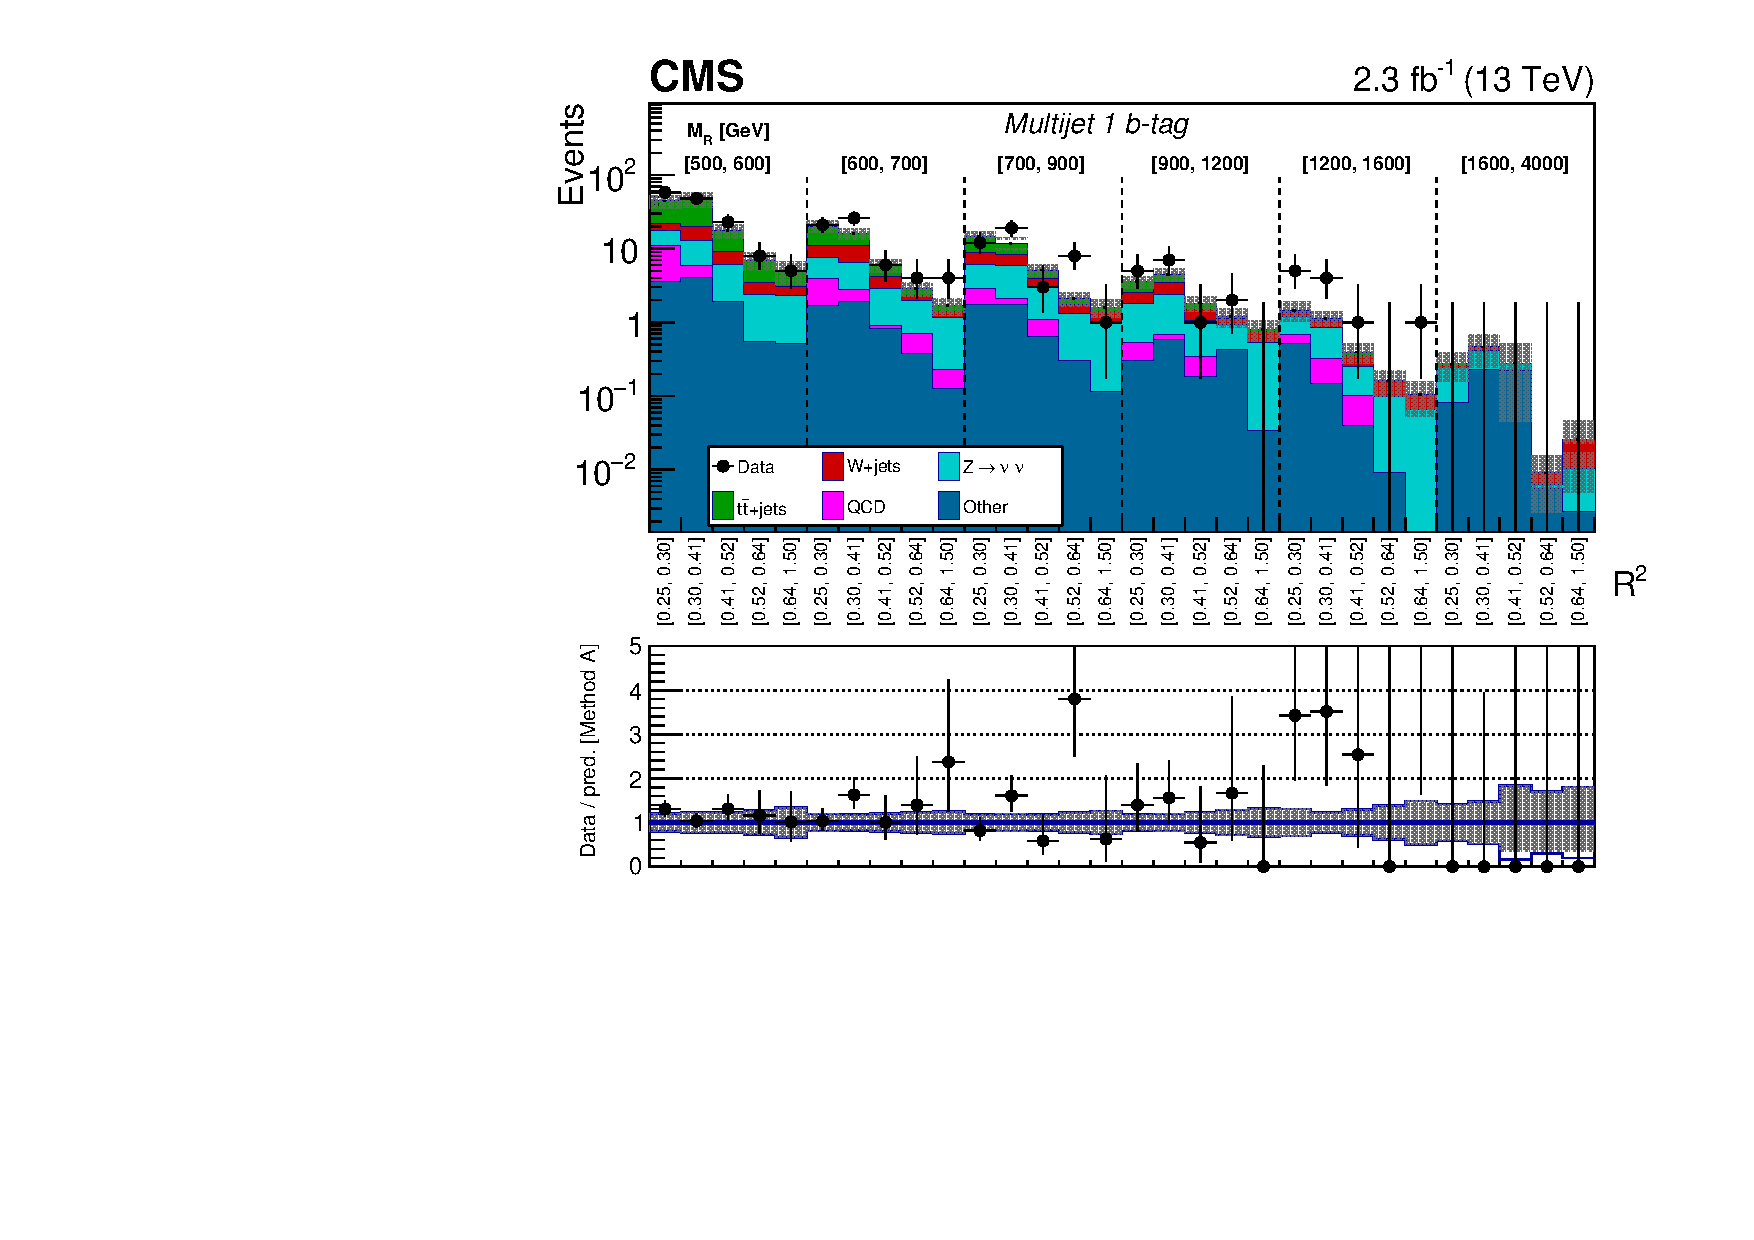
\includegraphics[width=0.8\textwidth]{figs/analysis13TeV/results/MRRsqMultiJet1BTagUnrolledDataMC.pdf}}
\caption{ The ($\MR$,$\Rtwo$) distribution observed in data is shown along with the background prediction
obtained from method A for the Multijet event category in the 0
\PQb-tag (upper) and 1 \PQb-tag (lower) bins~\cite{CMS-PAS-SUS-15-004}. The two-dimensional ($\MR$,$\Rtwo$) distribution is shown
in a one-dimensional representation, with each $\MR$ bin marked by the dashed lines and labeled near the top,
and each $\Rtwo$ bin labeled below. The ratio of data to the background
prediction is shown on the bottom panels, with
the statistical uncertainty expressed through the data point error bars and the systematic uncertainty of the
background prediction represented by the shaded region. 
}
\label{fig:ResultsMultiJet0btag1btag}
\end{figure}

\begin{figure}[!ptb] \centering
\subfigure{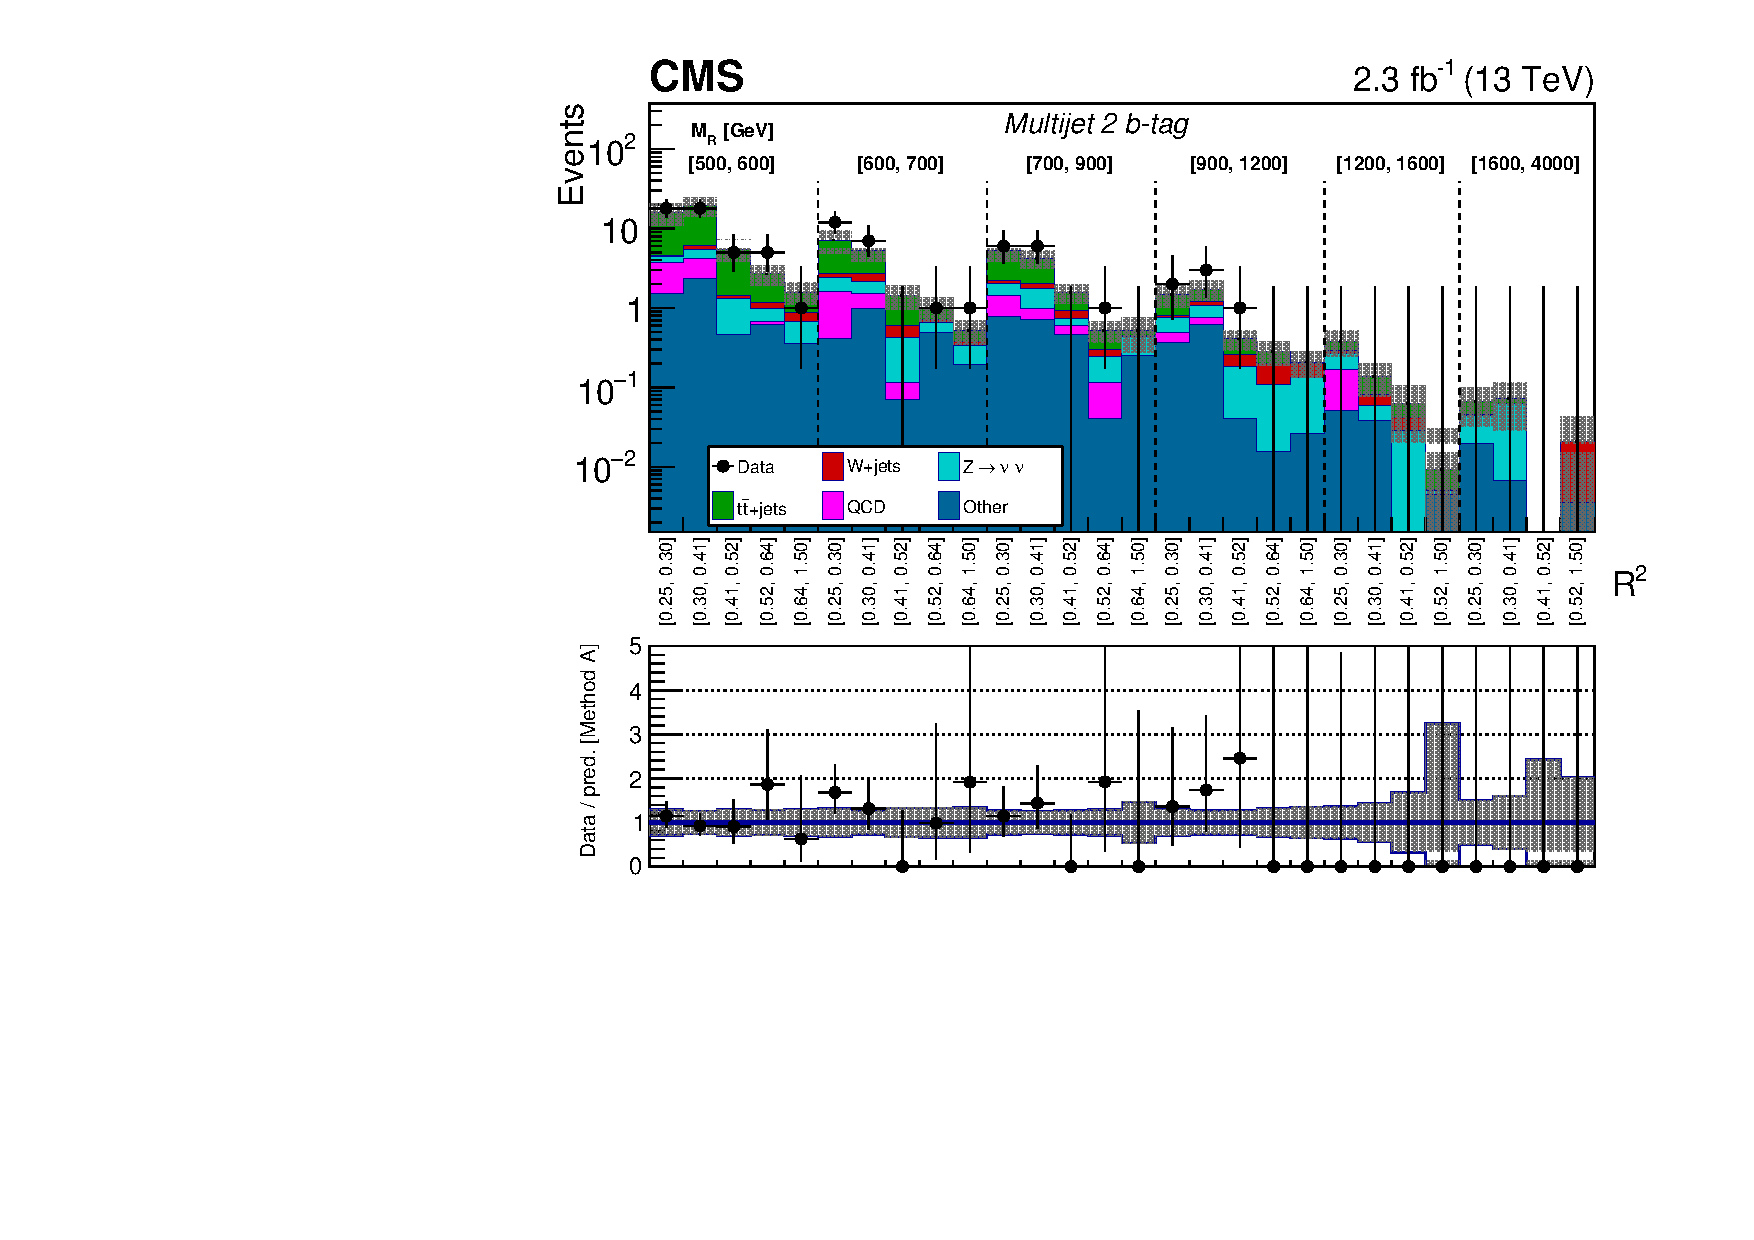
\includegraphics[width=0.8\textwidth]{figs/analysis13TeV/results/MRRsqMultiJet2BTagUnrolledDataMC.pdf}}\\
\subfigure{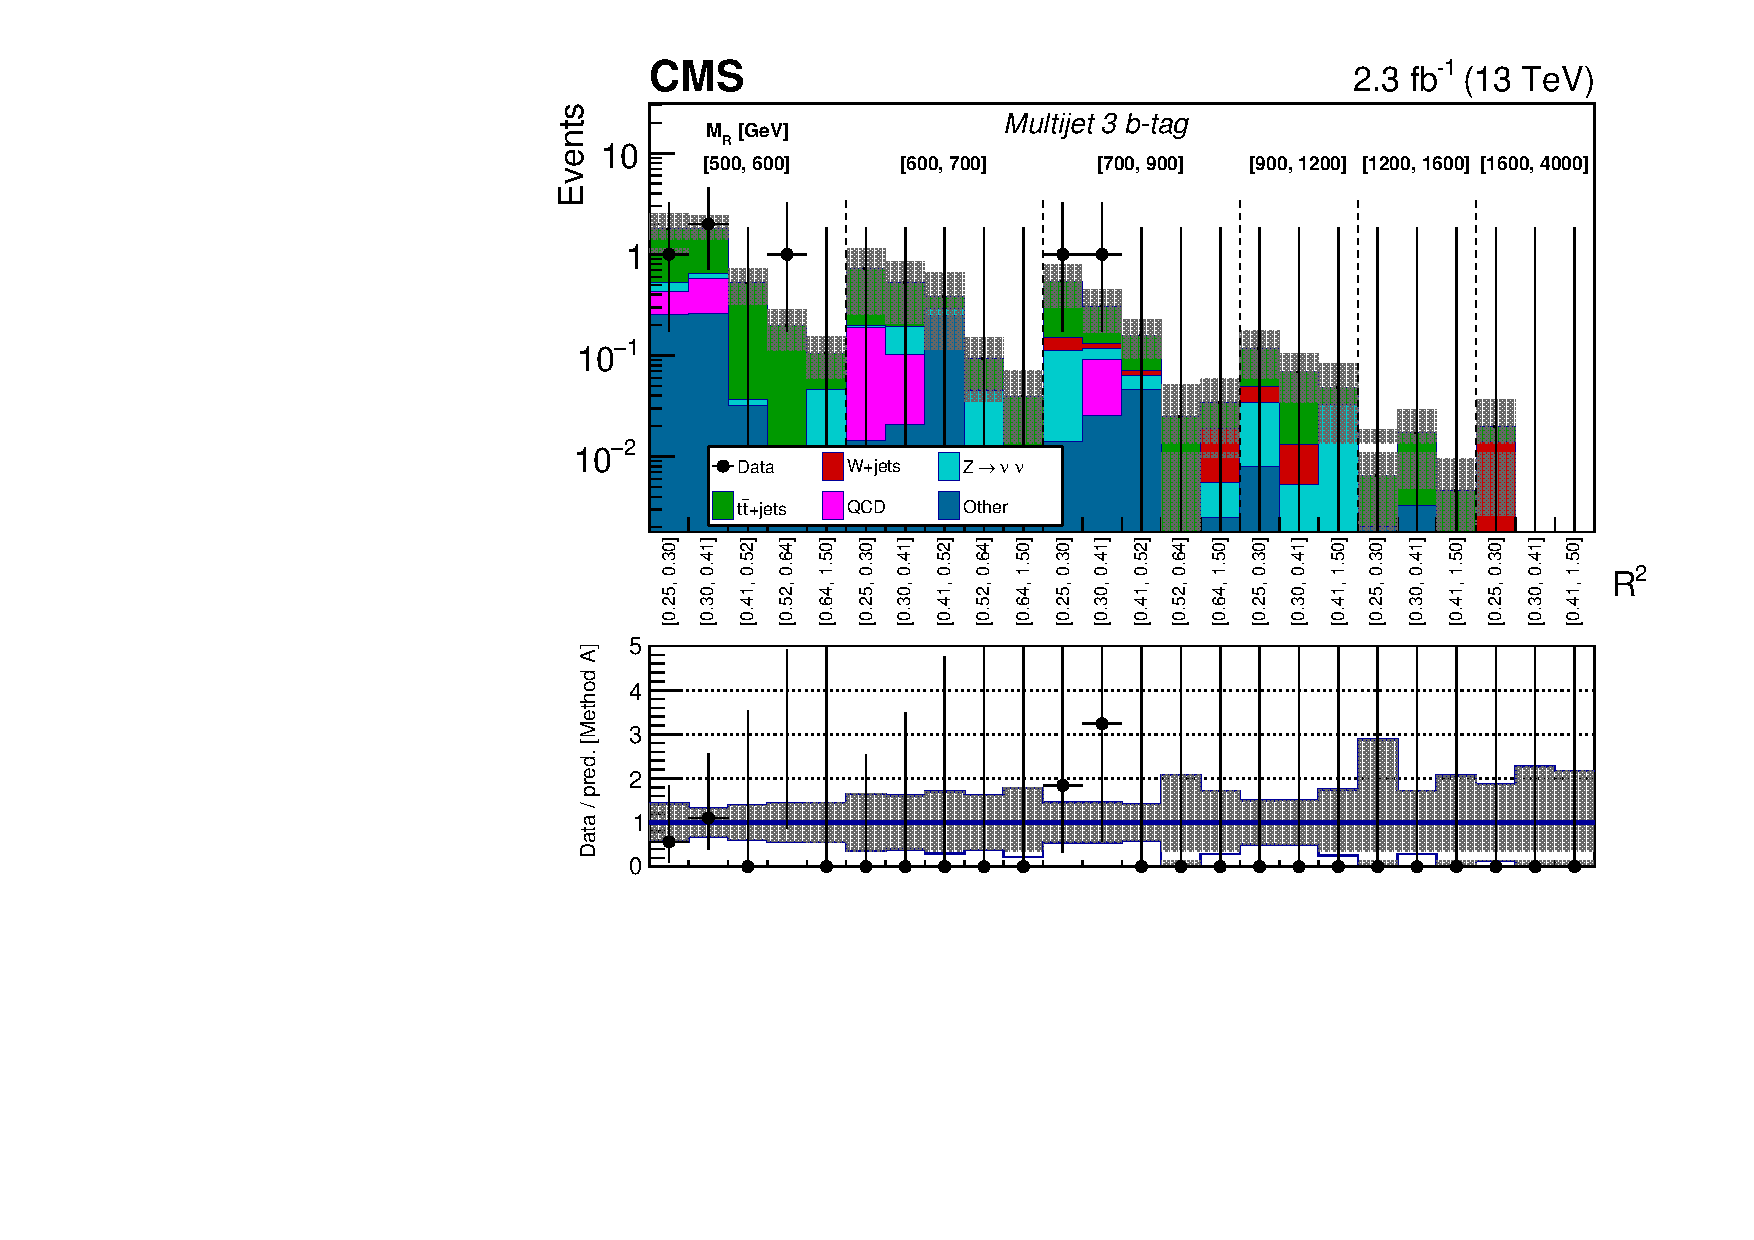
\includegraphics[width=0.8\textwidth]{figs/analysis13TeV/results/MRRsqMultiJet3BTagUnrolledDataMC.pdf}}
\caption{ The ($\MR$,$\Rtwo$) distribution observed in data is shown along with the background prediction
obtained from method A for the Multijet event category in the 2 \PQb-tag (upper) and $\geq 3$ \PQb-tag (lower) bins~\cite{CMS-PAS-SUS-15-004}. 
A detailed explanation of the panels is given in the caption of   Fig.~\ref{fig:ResultsMultiJet0btag1btag}.
}
\label{fig:ResultsMultiJet2btag3btag}
\end{figure}

\begin{figure}[!htb] \centering
\subfigure{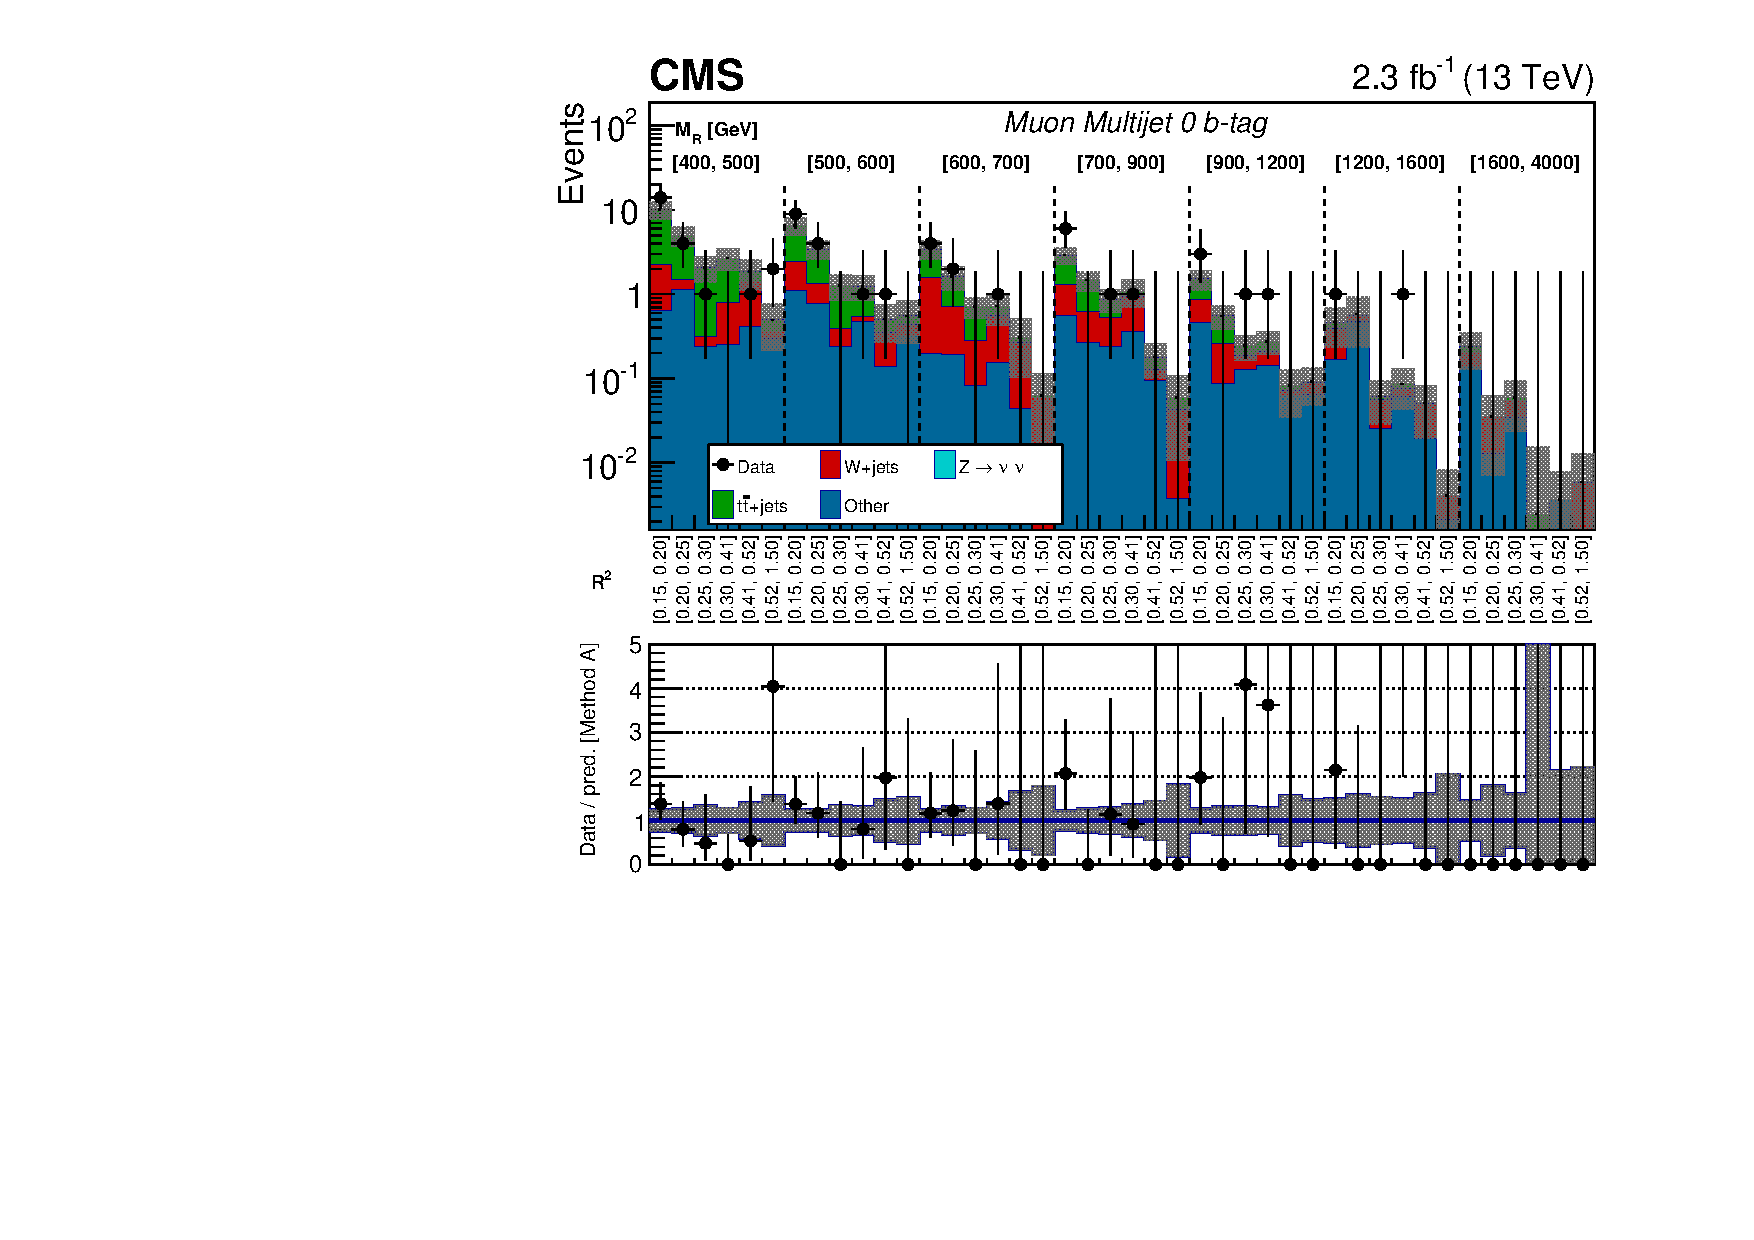
\includegraphics[width=0.8\textwidth]{figs/analysis13TeV/results/MRRsqMuMultiJet0BTagUnrolledDataMC.pdf}}\\
\subfigure{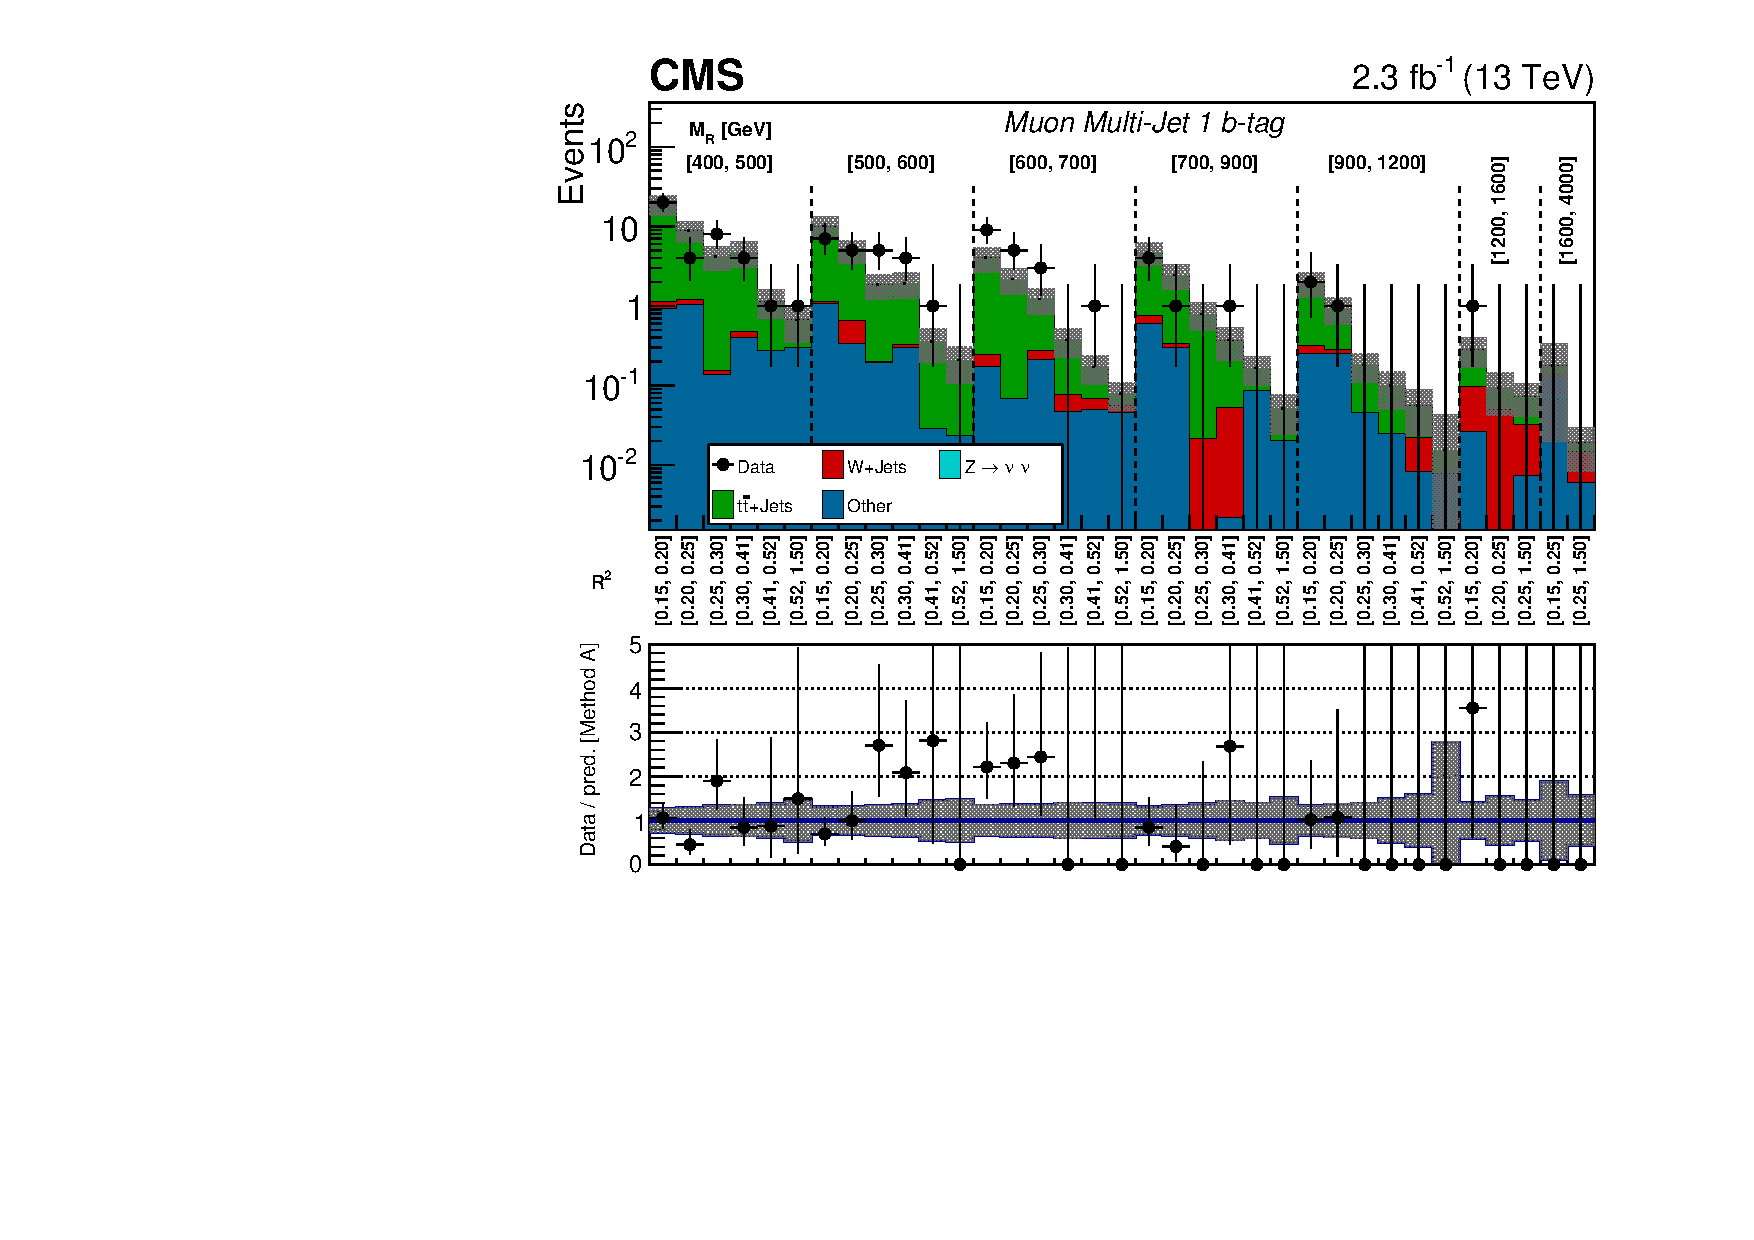
\includegraphics[width=0.8\textwidth]{figs/analysis13TeV/results/MRRsqMuMultiJet1BTagUnrolledDataMC.pdf}}
\caption{ The ($\MR$,$\Rtwo$) distribution observed in data is shown along with the background prediction
obtained from method A for the Muon Multijet event category in the 0 \PQb-tag (upper) and 1 \PQb-tag (lower) bins~\cite{CMS-PAS-SUS-15-004}. 
A detailed explanation of the panels is given in the caption of
  Fig.~\ref{fig:ResultsMultiJet0btag1btag}.
}
\label{fig:ResultsMuMultiJet0btag1btag}
\end{figure}

\begin{figure}[!ptb] \centering
\subfigure{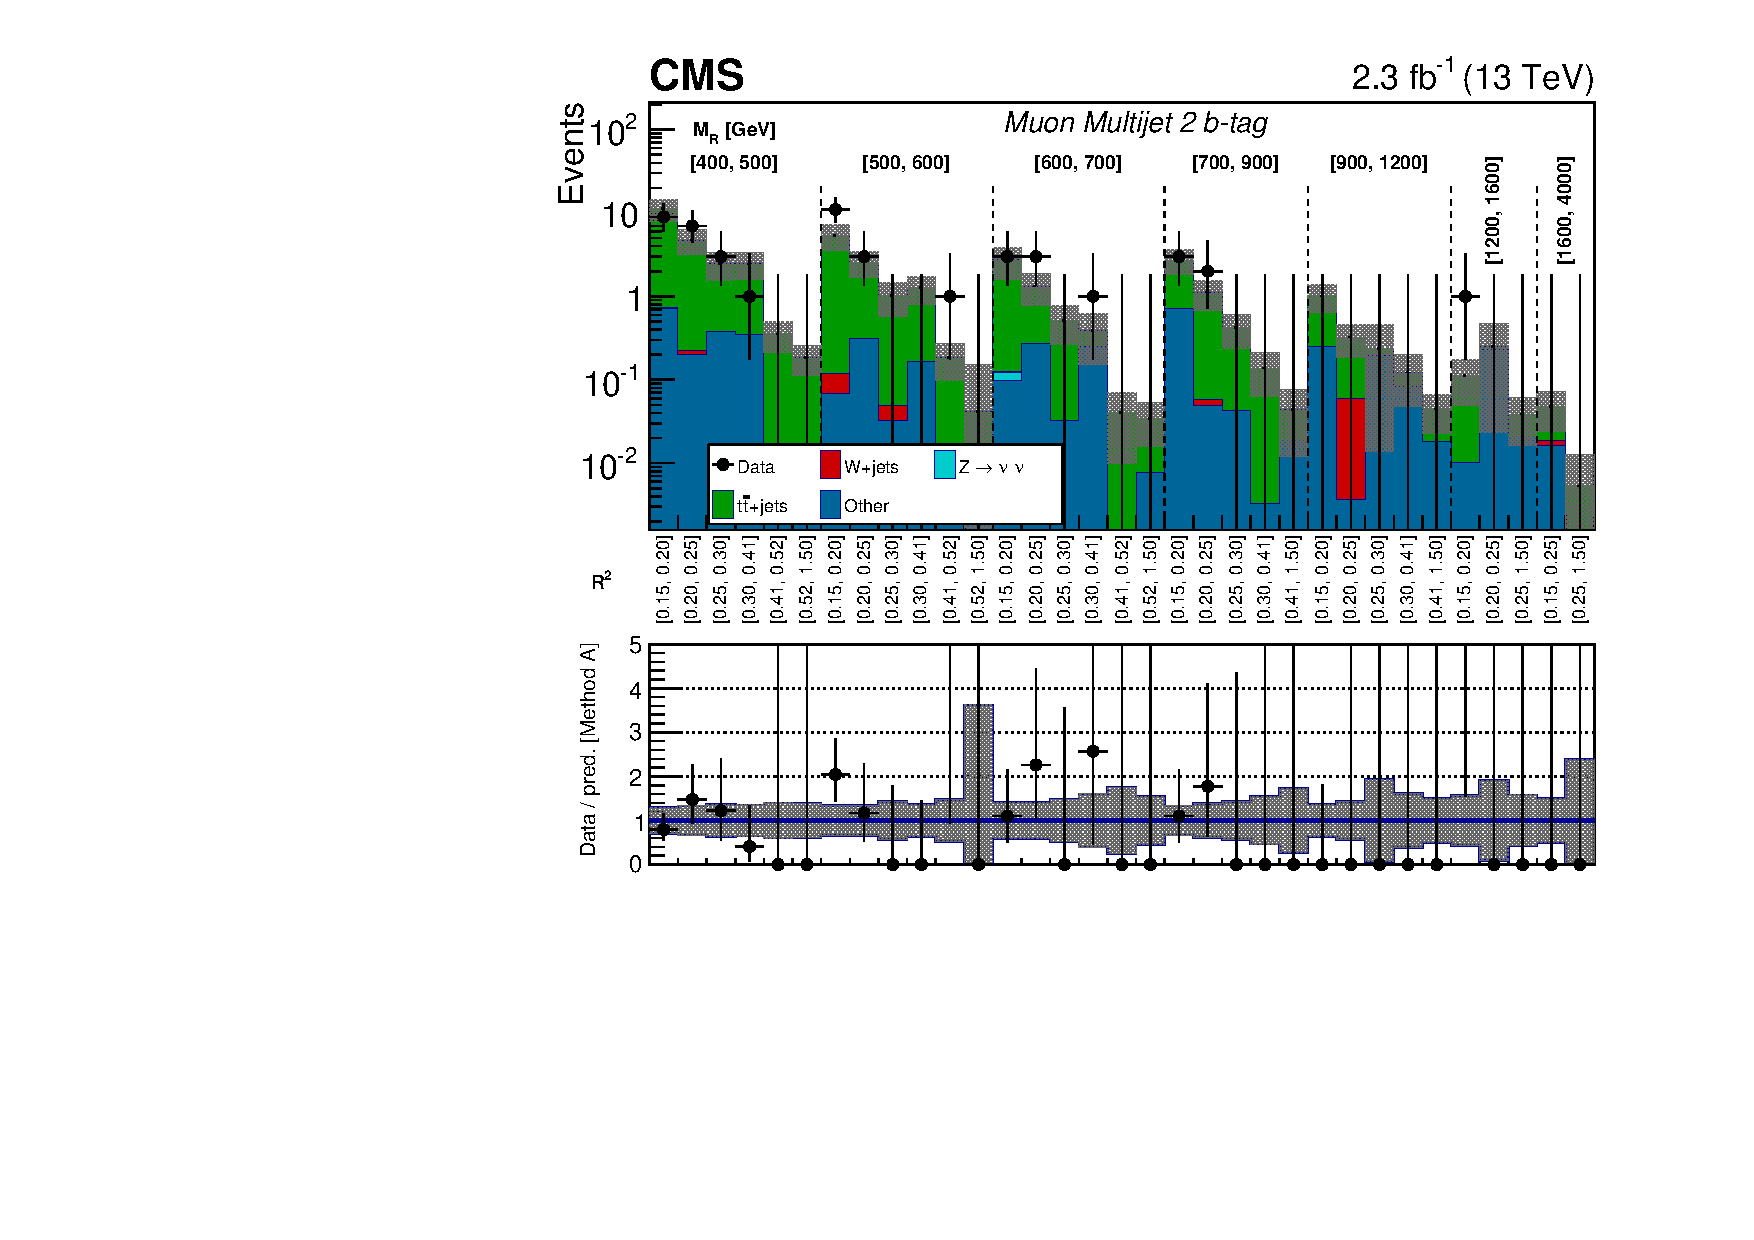
\includegraphics[width=0.8\textwidth]{figs/analysis13TeV/results/MRRsqMuMultiJet2BTagUnrolledDataMC.pdf}}\\
\subfigure{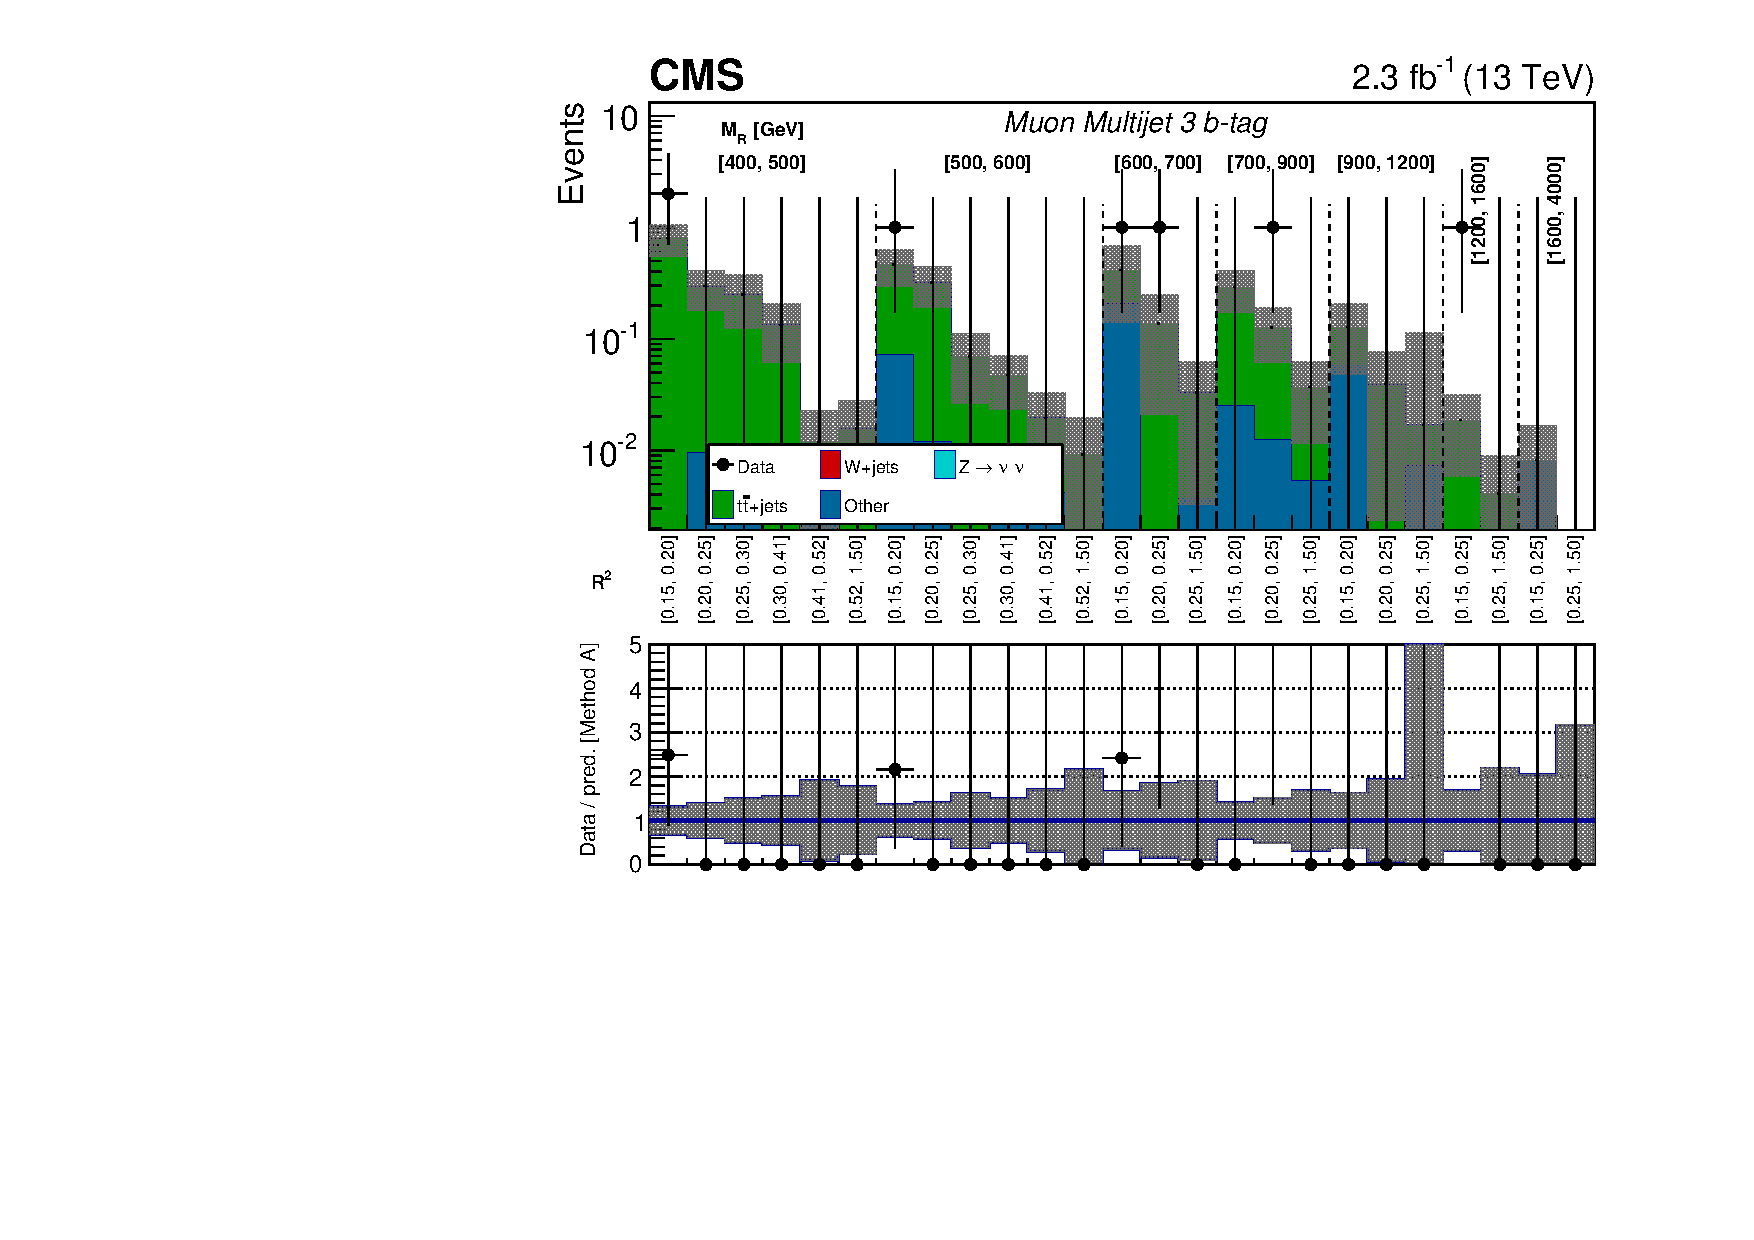
\includegraphics[width=0.8\textwidth]{figs/analysis13TeV/results/MRRsqMuMultiJet3BTagUnrolledDataMC.pdf}}
\caption{ The ($\MR$,$\Rtwo$) distribution observed in data is shown along with the background prediction
obtained from method A for the Muon Multijet event category in the 2 \PQb-tag (upper) and $\geq 3$ \PQb-tag (lower) bins~\cite{CMS-PAS-SUS-15-004}. 
A detailed explanation of the panels is given in the caption of
  Fig.~\ref{fig:ResultsMultiJet0btag1btag}.
}
\label{fig:ResultsMuMultiJet2btag3btag}
\end{figure}

\begin{figure}[!htb] \centering
\subfigure{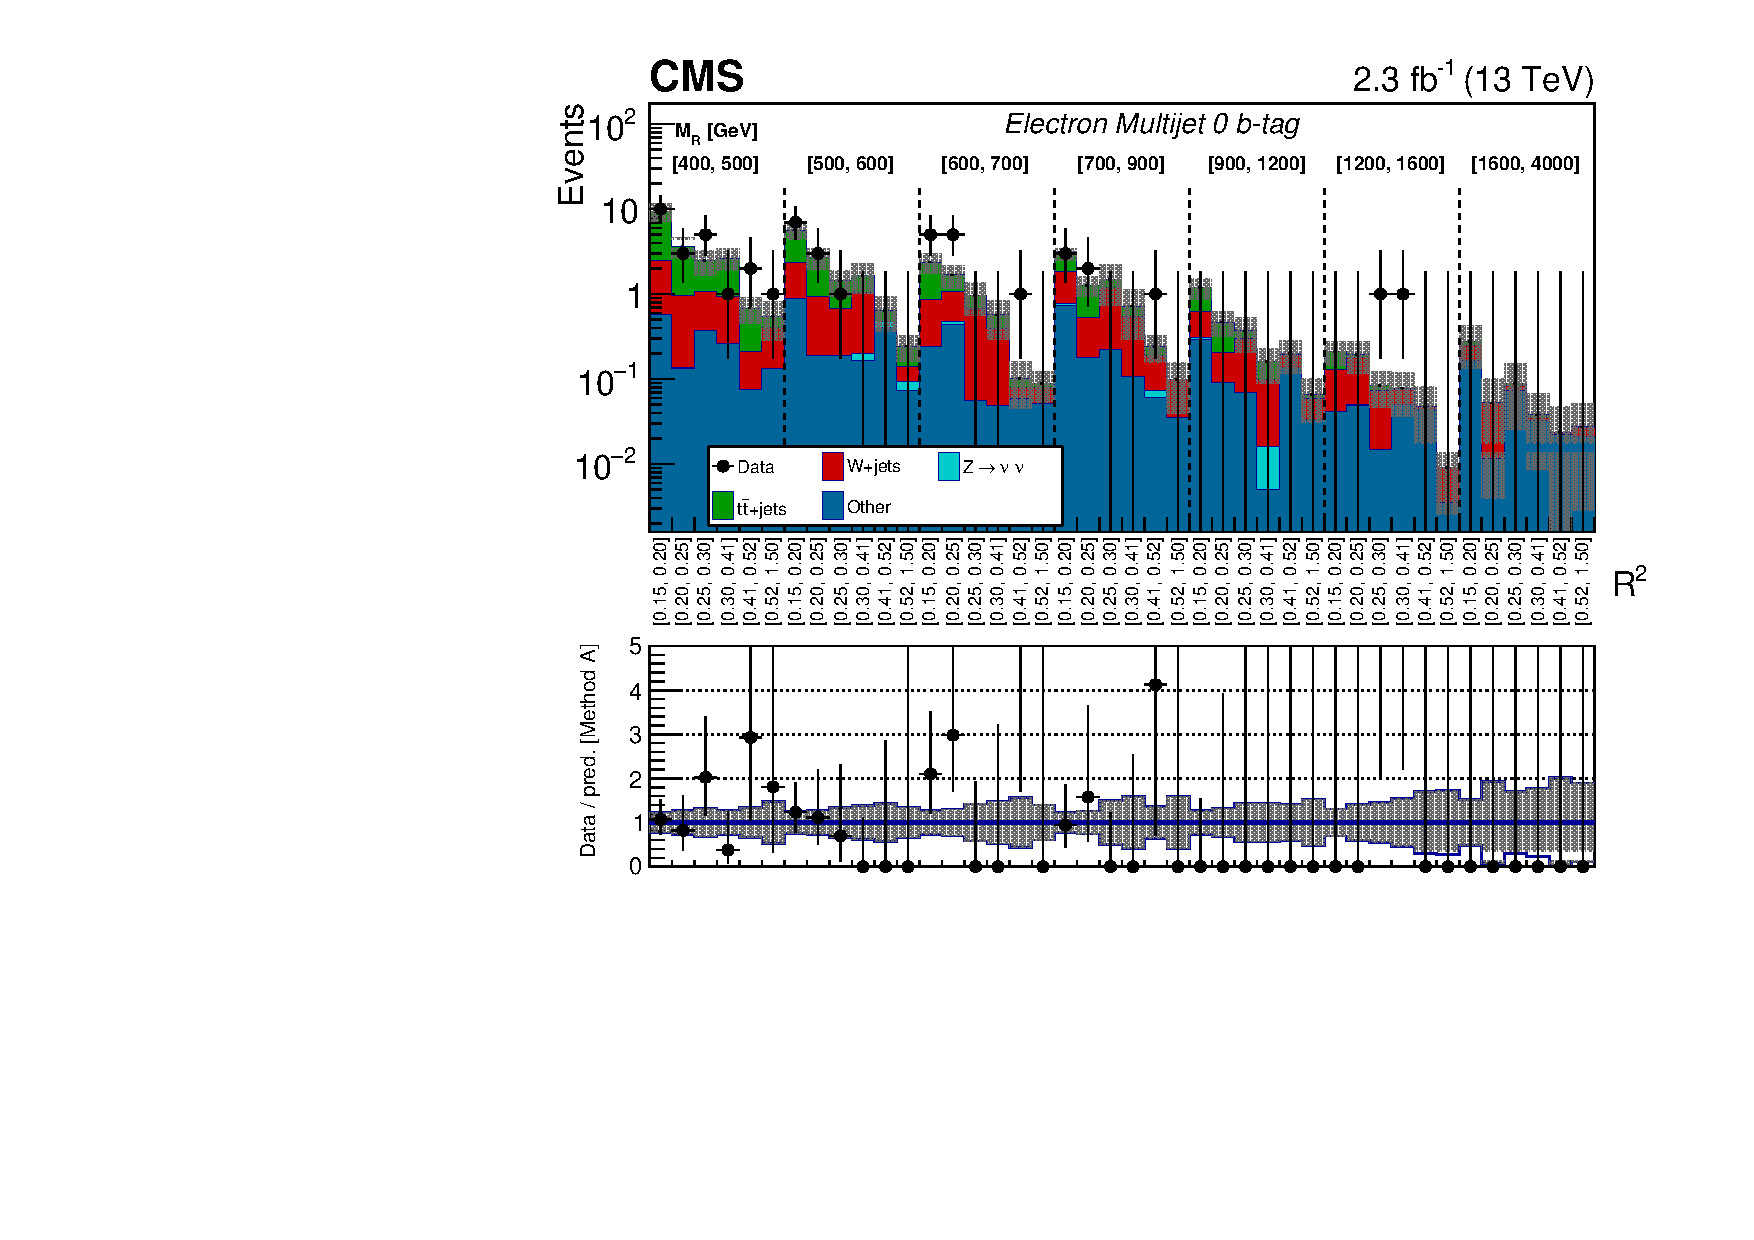
\includegraphics[width=0.8\textwidth]{figs/analysis13TeV/results/MRRsqEleMultiJet0BTagUnrolledDataMC.pdf}}\\
\subfigure{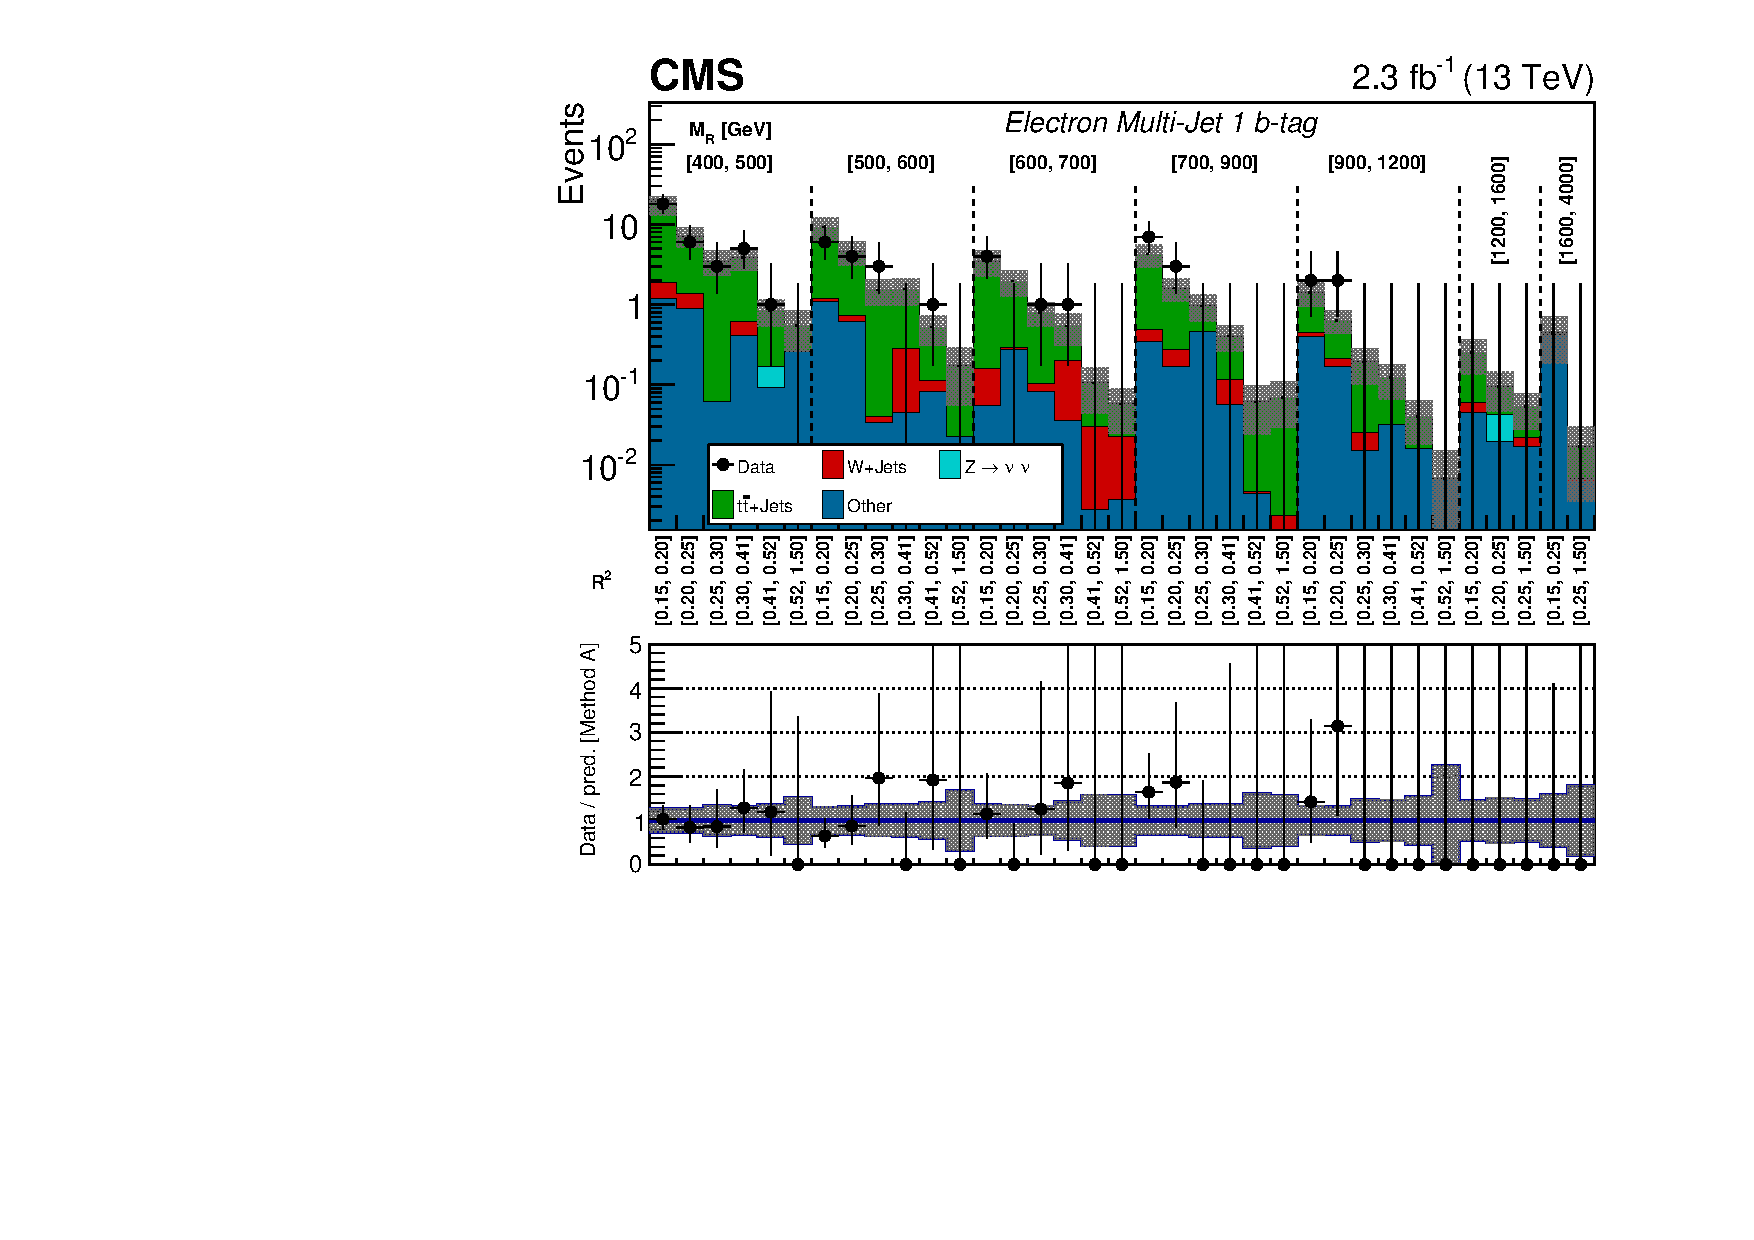
\includegraphics[width=0.8\textwidth]{figs/analysis13TeV/results/MRRsqEleMultiJet1BTagUnrolledDataMC.pdf}}
\caption{ The ($\MR$,$\Rtwo$) distribution observed in data is shown along with the background prediction
obtained from method A for the Electron Multijet event category in
the 0 \PQb-tag (upper) and 1 \PQb-tag (lower) bins. A detailed explanation of the panels is given in the caption of
  Fig.~\ref{fig:ResultsMultiJet0btag1btag}.
}
\label{fig:ResultsEleMultiJet0btag1btag}
\end{figure}

\begin{figure}[!htb] \centering
\subfigure{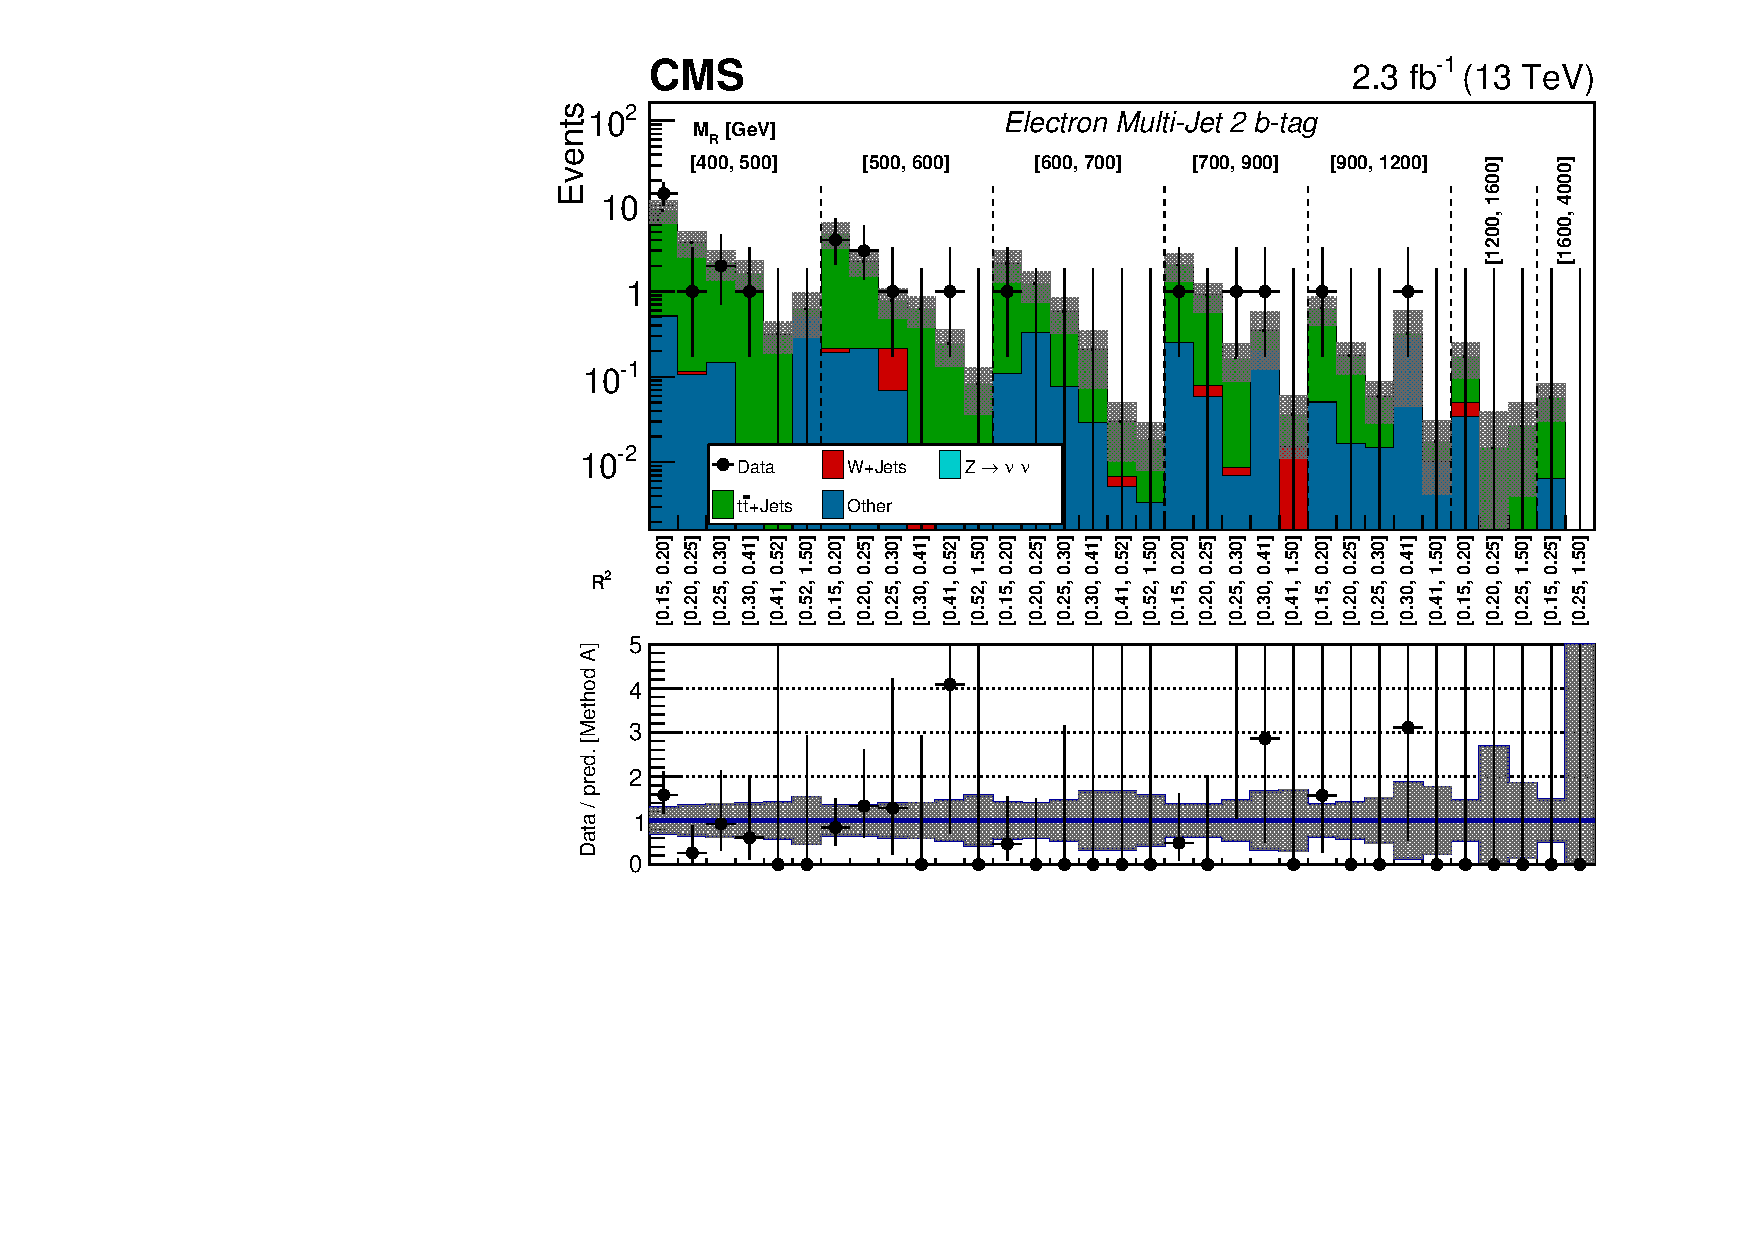
\includegraphics[width=0.8\textwidth]{figs/analysis13TeV/results/MRRsqEleMultiJet2BTagUnrolledDataMC.pdf}}\\
\subfigure{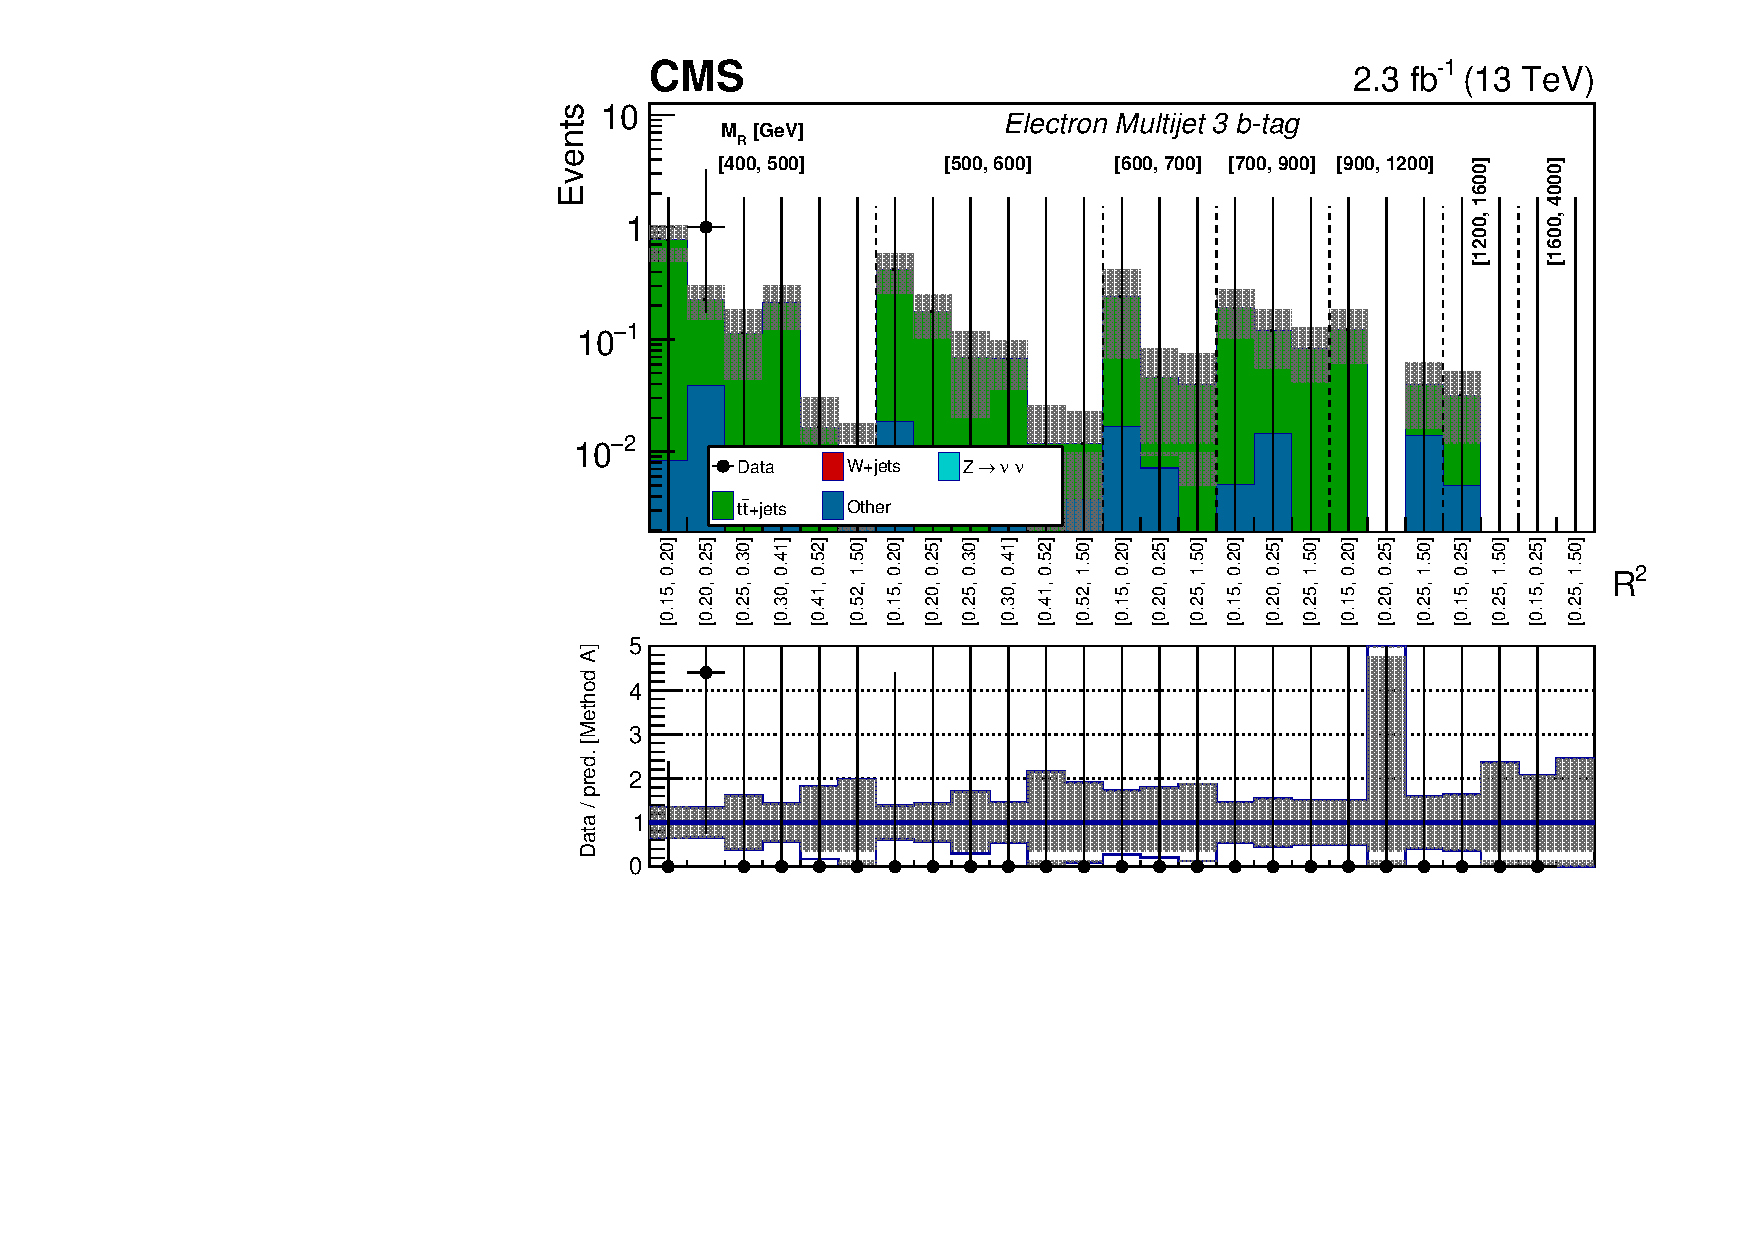
\includegraphics[width=0.8\textwidth]{figs/analysis13TeV/results/MRRsqEleMultiJet3BTagUnrolledDataMC.pdf}}
\caption{ The ($\MR$,$\Rtwo$) distribution observed in data is shown along with the background prediction
obtained from method A for the Electron Multijet event category in the 2 \PQb-tag (upper) and $\geq 3$ \PQb-tag (lower) bins~\cite{CMS-PAS-SUS-15-004}. 
A detailed explanation of the panels is given in the caption of Fig.~\ref{fig:ResultsMultiJet0btag1btag}.
}
\label{fig:ResultsEleMultiJet2btag3btag}
\end{figure}

\clearpage

First, we consider the scenario of gluino pair production
decaying to third-generation quarks. Gluino decays to the third-generation
are enhanced if the masses of the third-generation squarks are significantly
lighter than those of the first two generations, a scenario that is
strongly motivated in natural SUSY
models~\cite{naturalSUSY,Agashe:2014kda,DINE1990250,Cohen:1996vb} discussed in Sec.~\ref{sec:sms}. Prompted by this, we consider the three decay
modes: 
\begin{itemize}
\item $\PSg\rightarrow\bbbar\PSGcz$~;
\item $\PSg\rightarrow\ttbar\PSGcz$~; 
%\item $\PSg\rightarrow\cPqb\cPaqt\chip_1\rightarrow\cPqb\cPaqt \PW^{\ast+}\PSGcz_1$~or~$\PSg\rightarrow\cPaqb\cPqt\chim_1\rightarrow\cPaqb\cPqt \PW^{\ast-}\PSGcz_1$~. 
\item
  $\PSg\rightarrow\cPqb\cPaqt\chip_1\rightarrow\cPqb\cPaqt\PW^{\ast+}\PSGcz_1$~or
  charge conjugate,
\end{itemize}
where $\PW^{\ast}$ denotes a virtual $\PW$ boson. Due to a
technical limitation inherent in the event generator, we consider these
three decay modes for $\abs{m_{\sGlu}-m_{\chiz_1}} \geq 225 \GeV$. For
$\abs{m_{\sGlu}-m_{\chiz_1}} < 225 \GeV$, we only consider the $\PSg\rightarrow\bbbar\PSGcz$ decay mode. 

We perform a scan over all possible branching fractions to these three decay modes 
and compute limits on the production cross section under each such scenario. The production cross section
limits for a few characteristic branching fraction scan points are shown on the left of 
Fig.~\ref{fig:GluinoToThirdGenLimits} as a function of the gluino and neutralino masses. We find a range of excluded regions
for different branching fraction assumptions and generally observe the strongest limits for
the $\PSg\rightarrow\bbbar\PSGcz_1$ decay mode over the full two-dimensional mass plane
and the weakest limits for the $\PSg\rightarrow\ttbar\PSGcz_1$ decay
mode. For scenarios that include the intermediate decay
$\chipm_1\to\PW^{\ast \pm}\PSGcz_1$ and small values of $m_{\chiz_1}$ the sensitivity
is reduced because the LSP carries very little momentum in both the
NLSP rest frame and the laboratory frame, resulting in small values of
$\ETmiss$ and $\Rtwo$. By considering the most conservative limit obtained for all scanned branching fractions, we
calculate an exclusion limit valid for any assumption on the branching
fractions, presented on the right of Fig.~\ref{fig:GluinoToThirdGenLimits}. For
an LSP with mass of a few hundred $\GeV$, we exclude pair production of gluinos decaying 
to third-generation quarks for mass below about $1.6 \TeV$. This result 
is a unique attempt at deriving a branching fraction independent limit on
gluino pair production at the LHC for the scenario in which gluino decays are dominated by 
three-body decays to third-generation quarks and a neutralino LSP.


\begin{figure}[!ptb] \centering
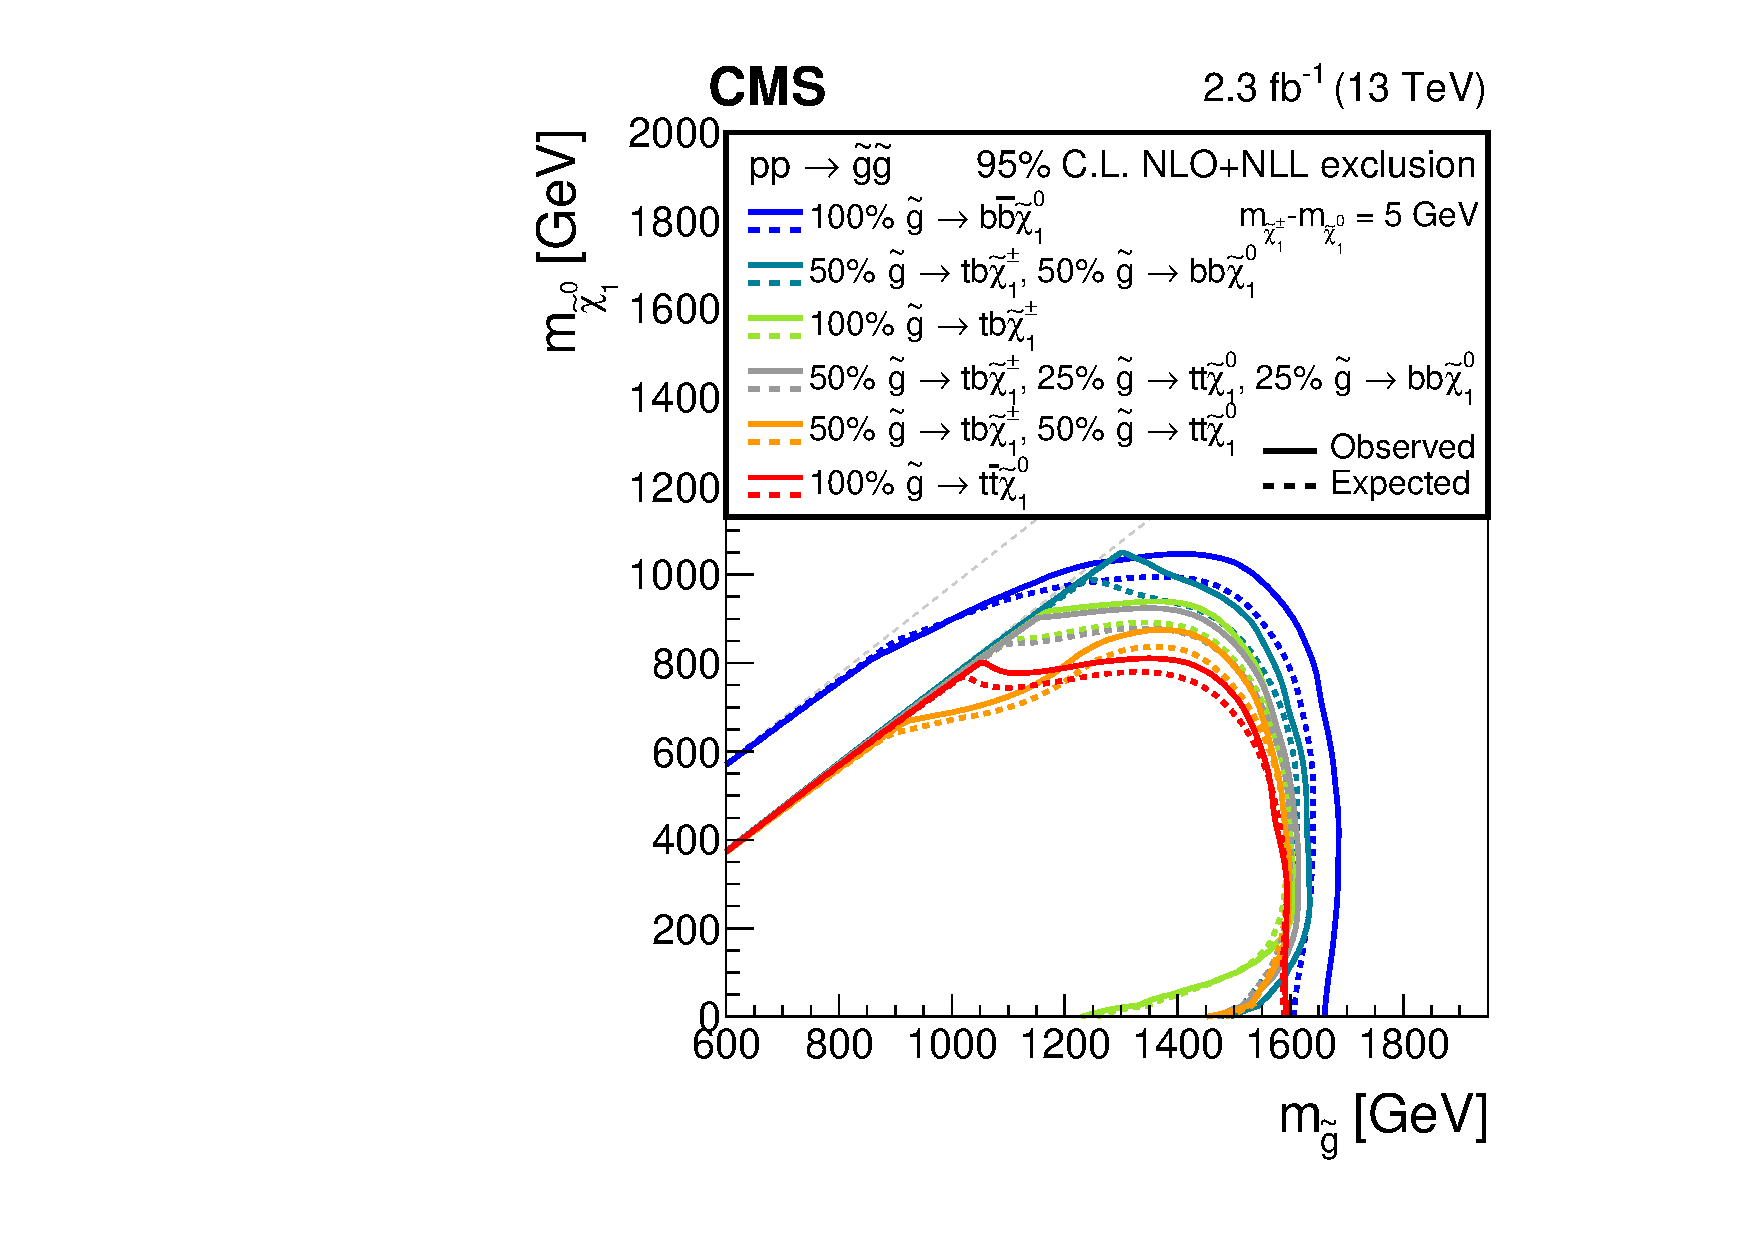
\includegraphics[width=0.49\textwidth]{figs/analysis13TeV/UnblindedResults/T1AsymptoticMADD.pdf}
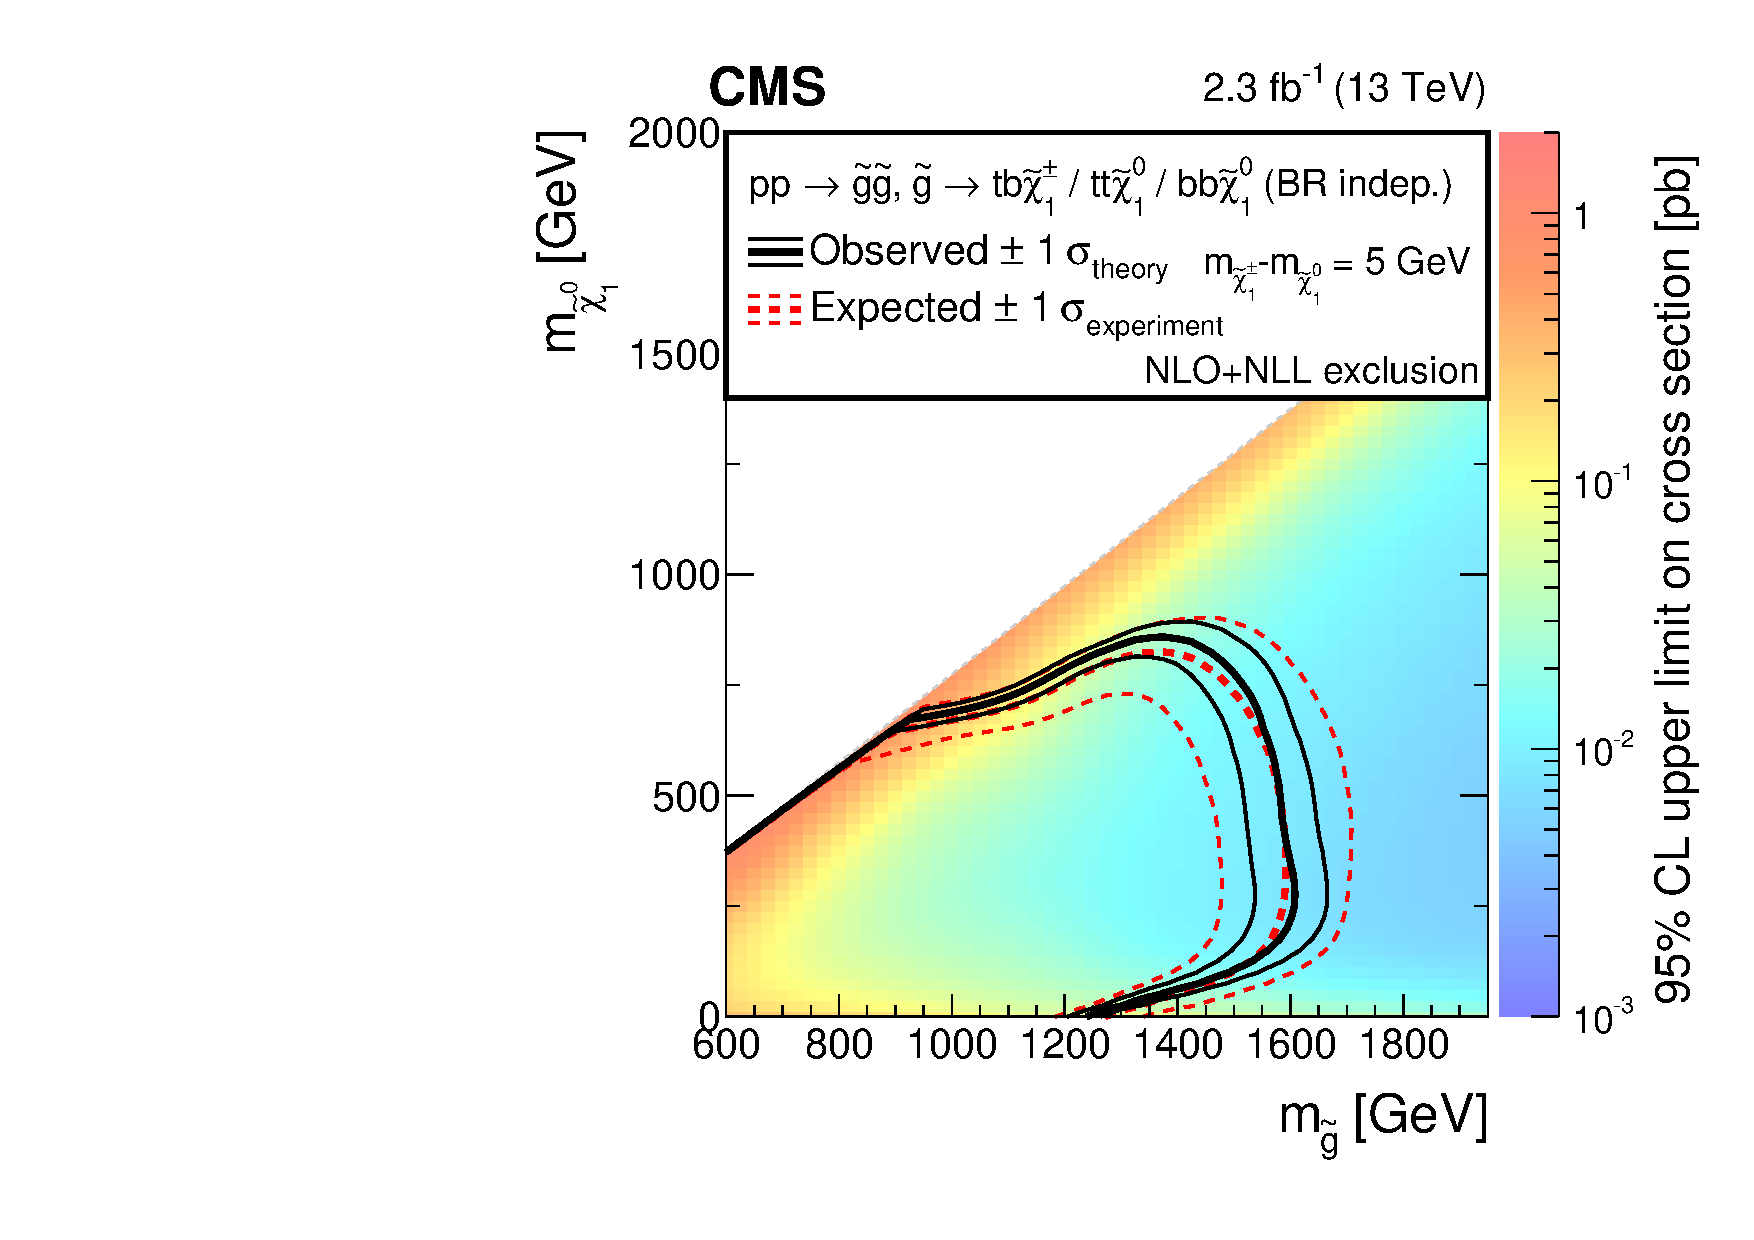
\includegraphics[width=0.49\textwidth]{figs/analysis13TeV/UnblindedResults/T1briFinalXSEC.pdf}
\caption{(Left) the expected and observed 95\% confidence level (CL) upper limits on the production 
cross section for gluino pair production decaying to third-generation quarks under various 
assumptions of the branching fractions. The two gray dashed diagonal
lines correspond to $\abs{m_{\sGlu}-m_{\chiz_1}} = 25 \GeV$, which is
where the scan ends for the $\sGlu\rightarrow\bbbar\chiz_1$ decay
mode, and $\abs{m_{\sGlu}-m_{\chiz_1}} = 225 \GeV$, which is where the scan
ends for the remaining modes due to a technical limitation inherent
in the event generator. For $\abs{m_{\sGlu}-m_{\chiz_1}} < 225 \GeV$,
we only consider the $\sGlu\rightarrow\bbbar\chiz_1$ decay mode. (Right) the analogous upper limits on 
the gluino pair production cross section valid for any values of the gluino
decay branching fractions~\cite{CMS-PAS-SUS-15-004}.
}
\label{fig:GluinoToThirdGenLimits}
\end{figure}


In Fig.~\ref{fig:limitT1qqqqT2tt}, we present additional interpretations for
simplified model scenarios of interest. On the left, we show the production cross section
limits on gluino pair production where the gluino decays to two light-flavored
quarks and the LSP, and on the right we show the production cross section limits on
top squark pair production where the top squark decays to a top quark and the LSP. 
For a very light LSP, we exclude top squark production with mass below
$750 \GeV$.

\begin{figure}[!htb] \centering
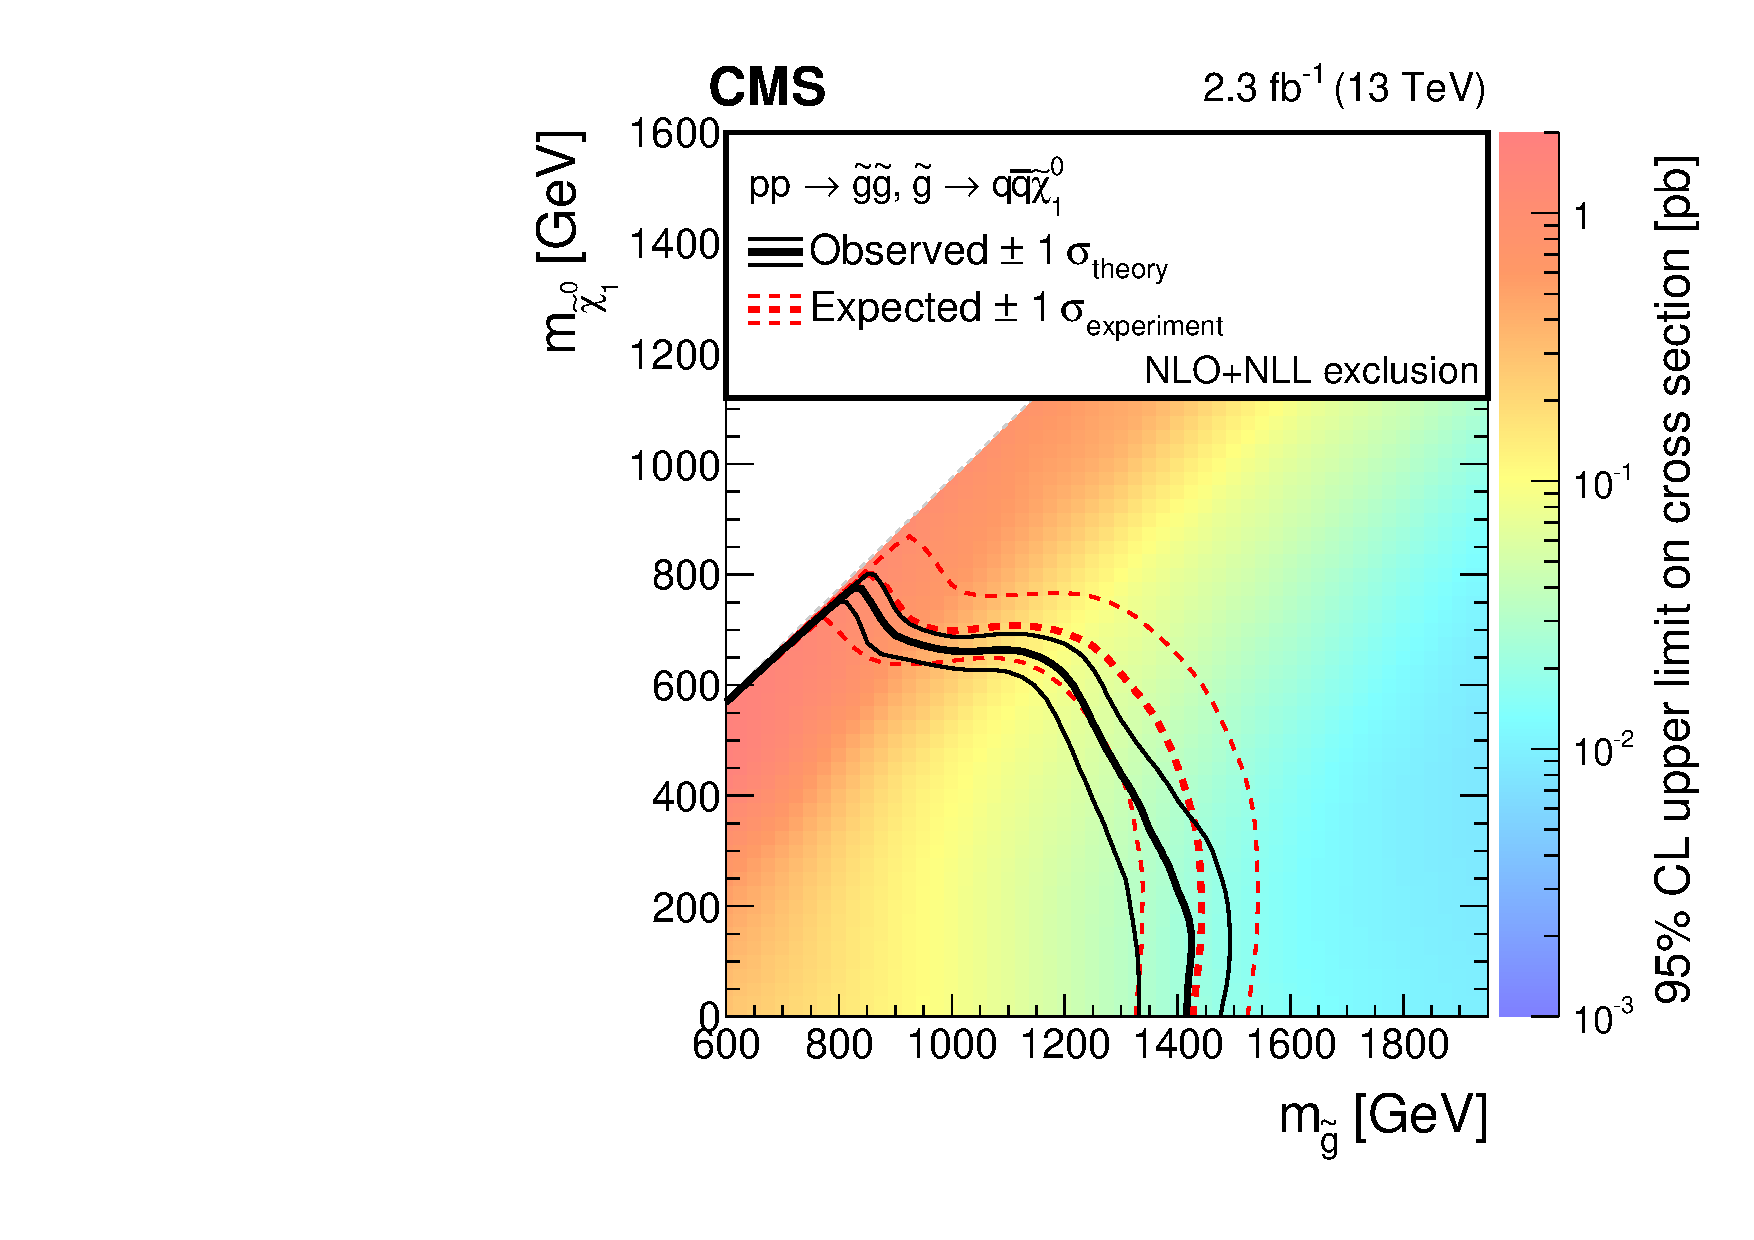
\includegraphics[width=0.49\textwidth]{figs/analysis13TeV/UnblindedResults/T1qqqqFinalXSEC.pdf}
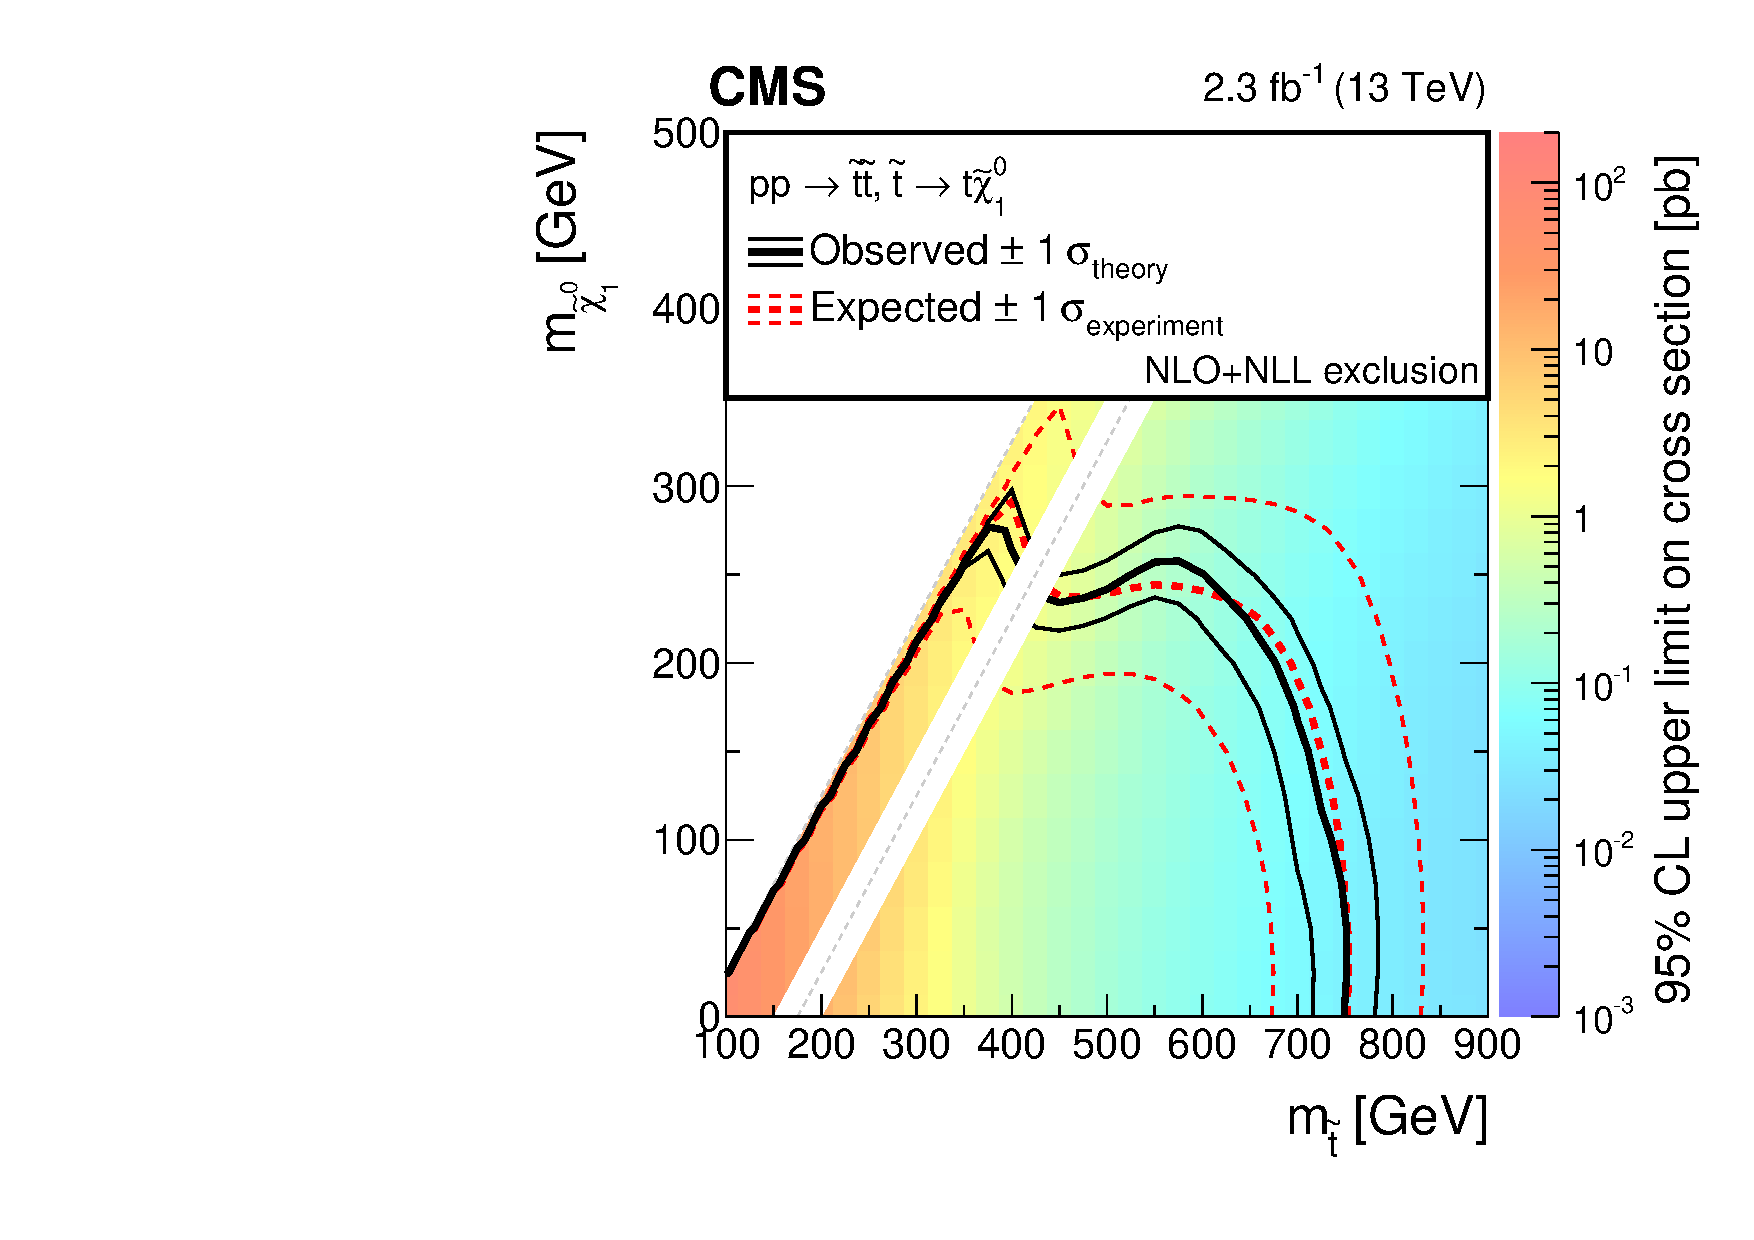
\includegraphics[width=0.49\textwidth]{figs/analysis13TeV/UnblindedResults/T2ttFinalXSEC.pdf}
\caption{ Expected and observed 95\% confidence level (CL) upper limits on the production cross section
for (left) gluino pair production decaying to two light-flavored quarks and the LSP
and (right) top squark pair production decaying to a top quark and the LSP. 
The white diagonal band in the right plot corresponds to the region
$\abs{m_{\sTop}-m_{\PQt}-m_{\chiz_1}} < 25 \GeV$, where the signal 
efficiency is a strong function of $m_{\sTop}-m_{\chiz_1}$, and as a 
result the precise determination of the cross section upper limit is uncertain
because of the finite granularity of the available MC samples 
in this region of the ($m_{\sTop}$, $m_{\chiz_1}$)  plane~\cite{CMS-PAS-SUS-15-004}.
}
\label{fig:limitT1qqqqT2tt}
\end{figure}


\section{Summary}
\label{sec:Summary}

We have presented an inclusive search for supersymmetry in events 
with no more than one lepton, a large multiplicity of energetic jets, and 
missing transverse energy. The search is sensitive to a broad
range of SUSY scenarios including pair production of gluinos and top
squarks. The event categorization in the number of leptons and 
the number of \PQb-tagged jets enhances the search sensitivity for a variety of different SUSY signal scenarios. 
Two alternative background estimation methods are presented, both
based on transfer factors between data control regions and the search
regions, but having very different systematic assumptions:
%Two alternative background estimation methods with very different 
%systematic assumptions are presented: 
one relying on the simulation and associated corrections derived in
the control regions, and the other relying on the accuracy of an
assumed functional form for the shape of background distribution in the $\MR$ and $\Rtwo$ variables.
The two predictions agree within their uncertainties, thereby
demonstrating the robustness of the background modeling. 

No significant deviations from the predicted standard model background are
observed in any of the search regions, and this result is interpreted
in the context of simplified models of gluino or top
squark pair production. For decays to a top quark and an LSP with a mass of $100\GeV$, we
exclude top squarks with masses below $750\GeV$. Considering
separately the decays to bottom quarks and the LSP or first- and
second-generation quarks and the LSP, gluino masses up to
$1.65\TeV$ or $1.4\TeV$ are excluded, respectively.
Furthermore, this search goes beyond the existing simplified model paradigm by
interpreting results in a broader context inspired by natural SUSY,
with multiple gluino decay modes considered simultaneously.
By scanning over all possible branching fractions
for three-body gluino decays to third generation quarks, exclusion
limits are derived on gluino pair production that are valid for any
values of the gluino decay branching fractions.
For a chargino NLSP nearly degenerate in mass with the LSP and LSP
masses in the range between $200$ and $600\GeV$, we exclude gluinos
with mass below $1.55$ to $1.6\TeV$, regardless of their decays. This
result is a more generic constraint on gluino production than
previously reported at the LHC. 

\section{LHC coverage of natural supersymmetry}
\label{sec:Coverage}
Although the results of the
Ch.~\ref{ch:analysis8TeV}~and~\ref{ch:analysis13TeV} represent the
most generic constaints on the gluino and top squark from the LHC in
terms of constraining multiple decay modes simultaneously, more stringent
constraints for particular decay modes have been derived. Fig.~\ref{fig:ICHEP2016Summary} shows the most
stringent limits on the gluino and top squark from ATLAS and CMS using
13\TeV data collected in 2016.

\begin{figure}[!htb] \centering
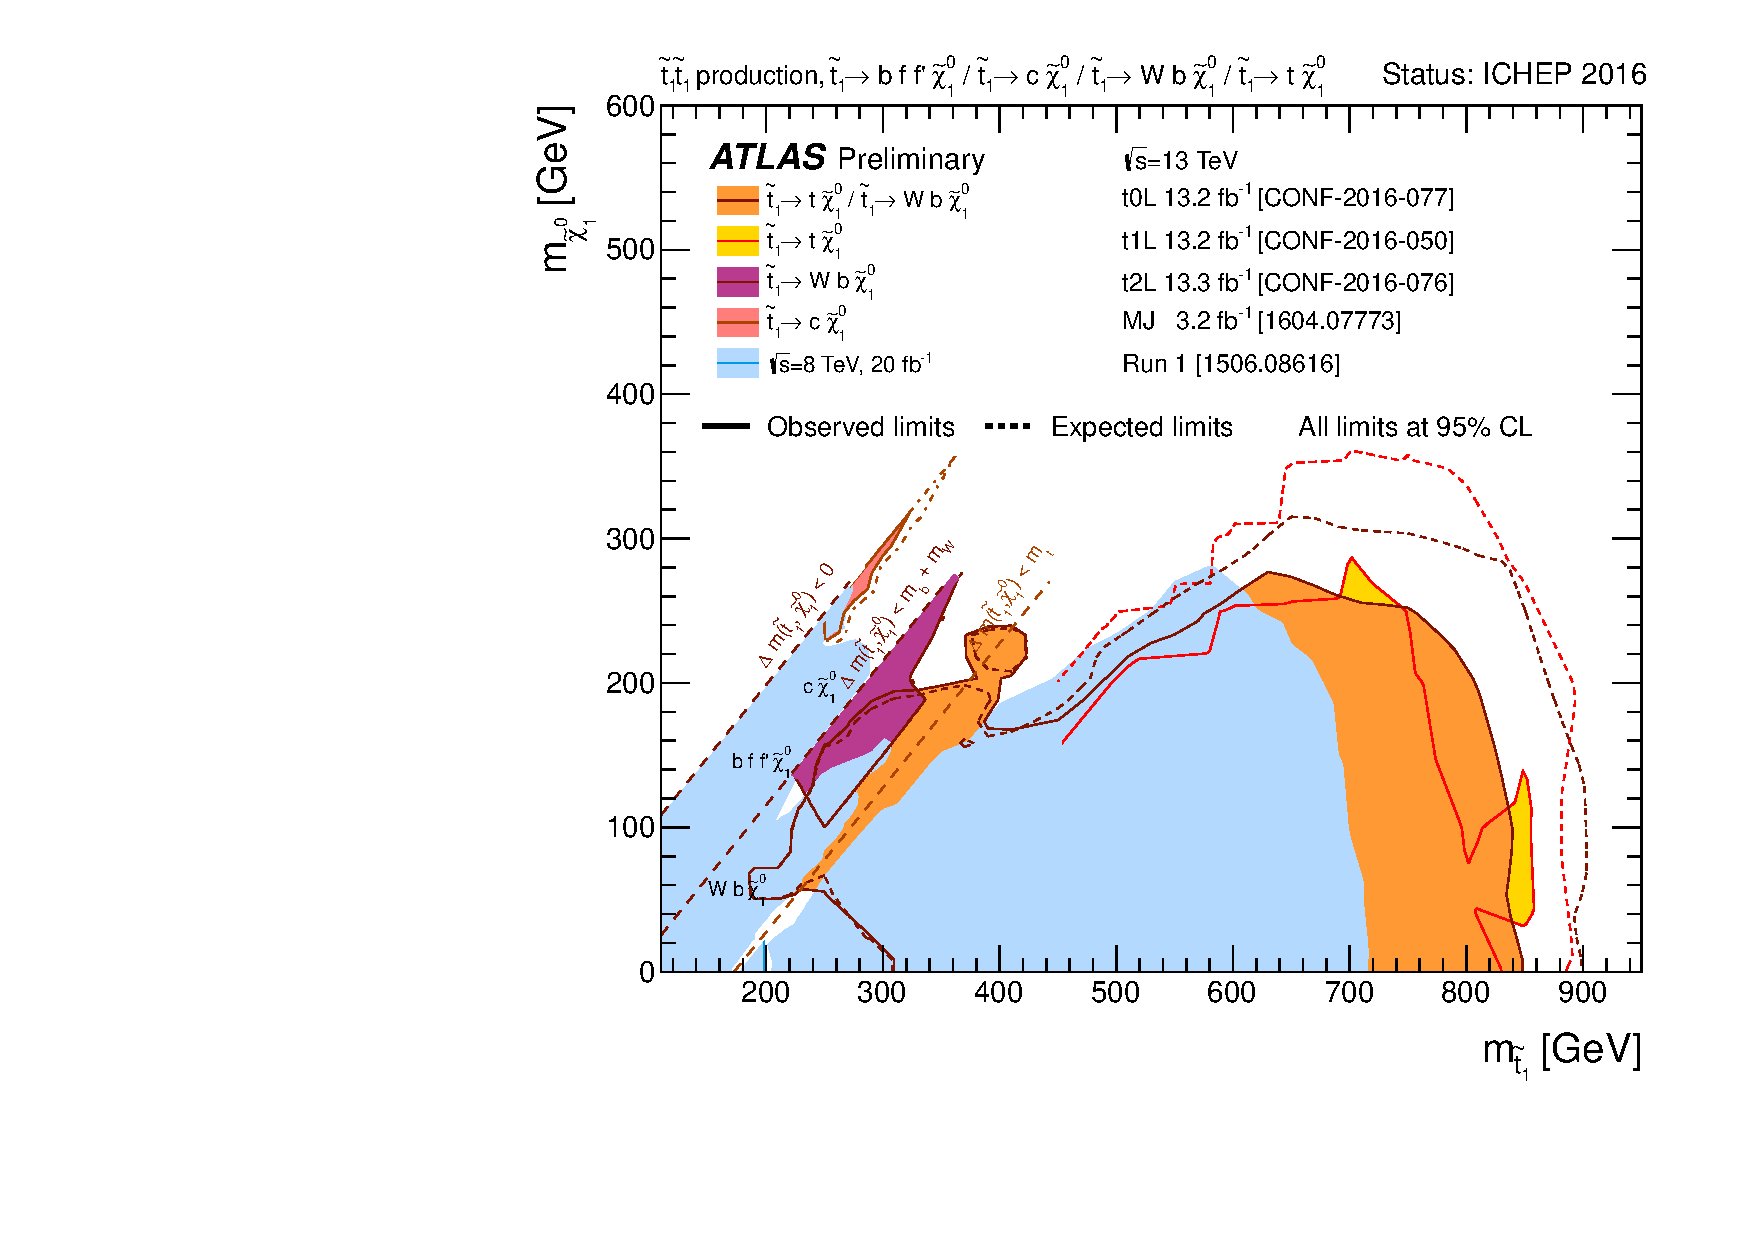
\includegraphics[width=0.49\textwidth]{figs/summary/ATLAS_SUSY_Stop_tLSP.pdf}
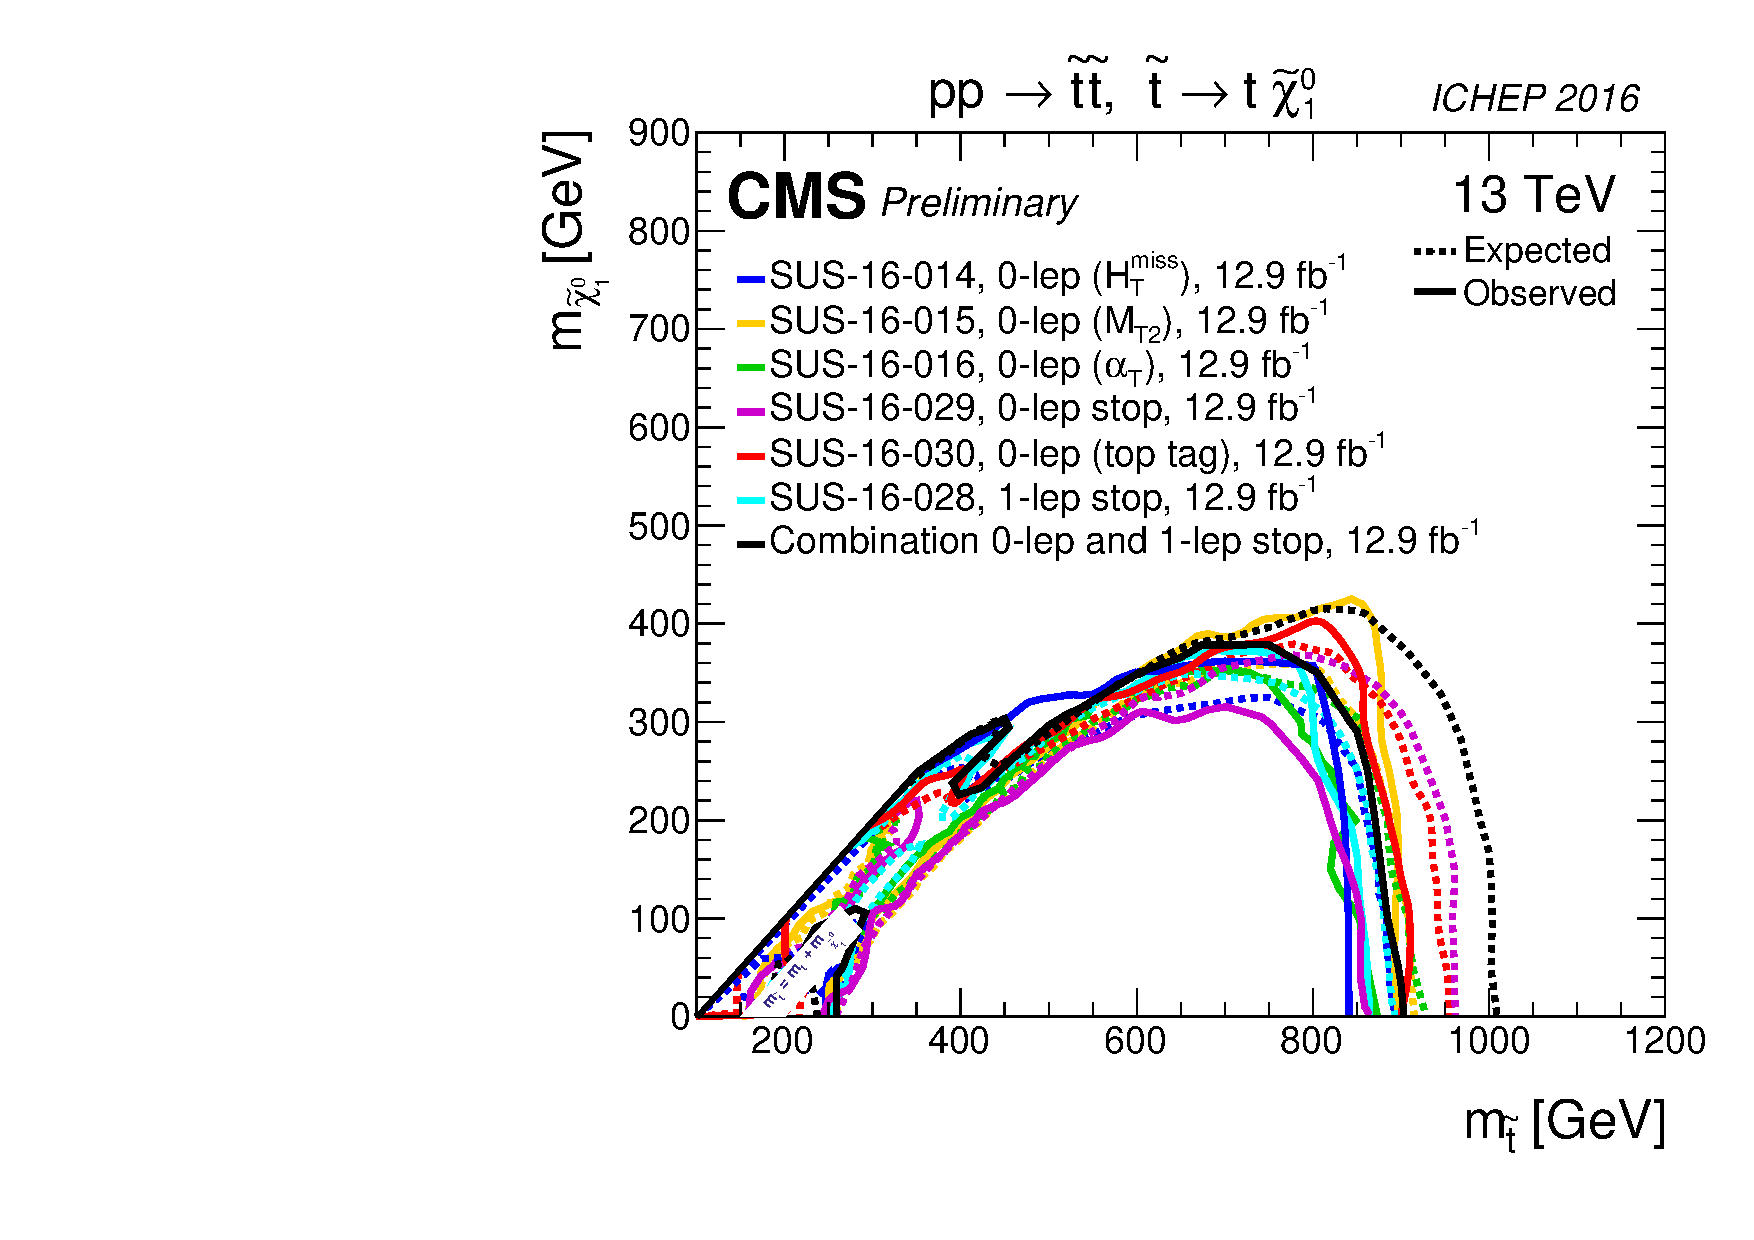
\includegraphics[width=0.49\textwidth]{figs/summary/T2tt_limits_summary_cms_ICHEP16.pdf}\\
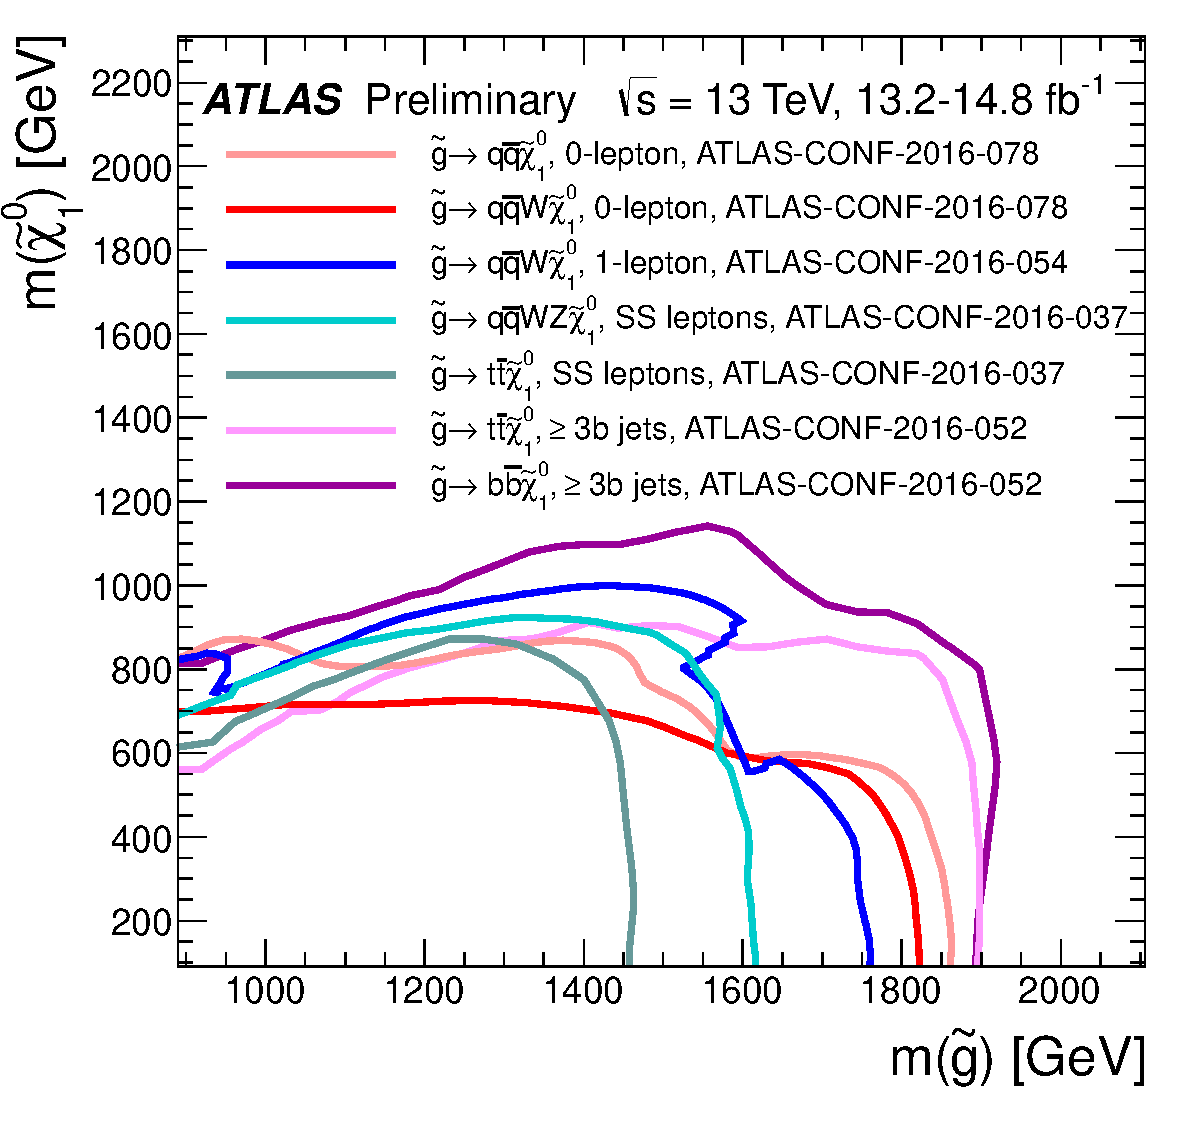
\includegraphics[width=0.49\textwidth]{figs/summary/ATLAS_SUSY_Strong_all.pdf}
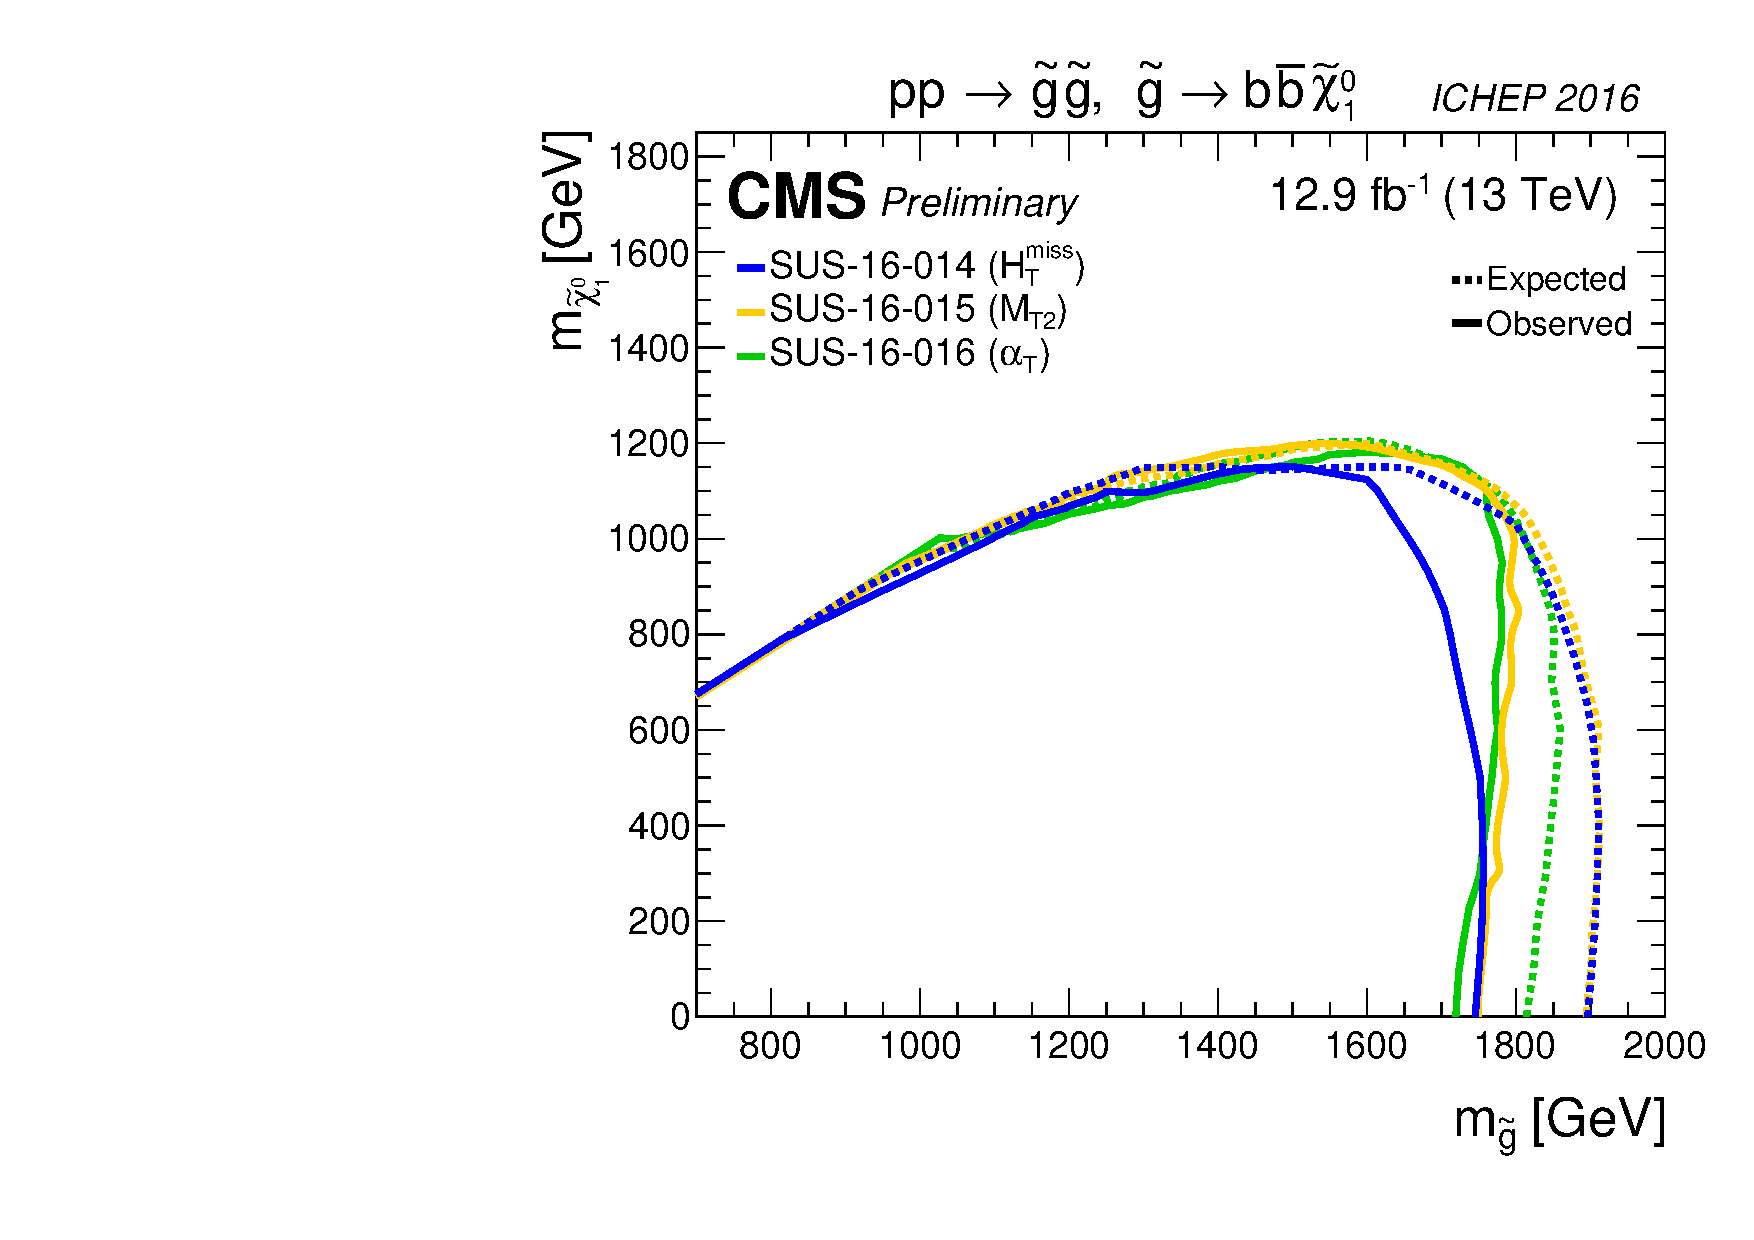
\includegraphics[width=0.49\textwidth]{figs/summary/T1bbbb_limits_summary_cms_ICHEP16.pdf}
\caption{ATLAS (left) and CMS (right) 13\TeV limits presented
  at ICHEP 2016 for top squark (top) and gluino (bottom) pair production.
\label{fig:ICHEP2016Summary}}
\end{figure}
